\documentclass[11pt]{article} % use larger type; default would be 10pt

\usepackage{lineno}
\usepackage{epsfig}
\usepackage{amsmath}
\usepackage{authblk}
\usepackage{multirow}
\usepackage{fancyhdr}
\usepackage[margin=2.5cm]{geometry} % to change the page dimensions
\usepackage{epstopdf}
\usepackage{graphicx} % support the \includegraphics command and options
\usepackage{color}
\usepackage{cancel}

%%% PACKAGES
\usepackage{booktabs} % for much better looking tables
\usepackage{array} % for better arrays (eg matrices) in maths
\usepackage{paralist} % very flexible & customisable lists (eg. enumerate/itemize, etc.)
\usepackage{verbatim} % adds environment for commenting out blocks of text & for better verbatim
\usepackage{subfig} % make it possible to include more than one captioned figure/table in a single float

\def \p0d{P\cancel{0}D}

%%% HEADERS & FOOTERS

%%% SECTION TITLE APPEARANCE
%\usepackage{sectsty}
%\allsectionsfont{\sffamily\mdseries\upshape} % (See the fntguide.pdf for font help)
% (This matches ConTeXt defaults)

%%% ToC (table of contents) APPEARANCE
\usepackage[nottoc,notlof,notlot]{tocbibind} % Put the bibliography in the ToC
\usepackage[titles,subfigure]{tocloft} % Alter the style of the Table of Contents
\renewcommand{\cftsecfont}{\rmfamily\mdseries\upshape}
\renewcommand{\cftsecpagefont}{\rmfamily\mdseries\upshape} % No bold!

%%% END Article customizations

%%% The "real" document content comes below...

\begin{document}
\linenumbers
\newcommand{\DocN}{T2K TN-080 V4}
\newcommand{\titlename}{
Analysis of $\nu_{\mu}$ Charged Current Inclusive Events in the \p0d \\
in Run 1+2+3+4}
\newcommand{\mc}[2]{\multicolumn{#1}{c}{#2}}
\pagestyle{fancy} % options: empty , plain , fancy
\lhead{Inclusive $\nu_{\mu}$ CC events in the \p0d in Run 1+2+3+4}
\rhead{\DocN}

\rfoot{T2K TN-080 V4}

\title{\titlename \\ {\small \DocN}}
\author[1]{Alex Clifton}
\author[1]{Rajarshi~Das}
\author[2]{Rob A.~Johnson}
\author[2]{Alysia D.~Marino}
\author[1]{Erez~Reinherz-Aronis}
\author[1]{Walter~Toki}
\author[2]{Tianlu~Yuan}
\affil[1]{\footnotesize \em Colorado State University, Fort Collins, Colorado, USA}
\affil[2]{\footnotesize \em University of Colorado, Boulder, Colorado, USA}



\maketitle

\begin{abstract}

We present an analysis of Charged
Current inclusive neutrino interactions that originate 
in the Pi-Zero Detector and have a % the secondary
negative %muon 
track reconstructed in the Time Projection Chamber. 
This analysis includes the ND280 Run 1-4 periods 
and utilized Production 5 samples both for Data and Monte Carlo.
The full data sample, which correspond to $56.8 \times 10^{19}$ 
Protons On Target, includes both the time periods 
where the \p0d water target
bags were filled and empty. %in both Run 1 and Run 2 (until February 13, 2011).
The analysis was performed at both the oaAnalysis and oaRecon levels 
with \p0d and Tracker reconstruction objects in conjunction with 
a Tracker to \p0d track matching algorithm. 
We report the result as a Data to Monte Carlo ratio of 
the total number of selected Charged Current inclusive interactions 
%n Run 1, Run 2 and Run 4 combined 
for the period where the water bags were fill and empty,
which we measure as  
%Using the Monte Carlo tuned beam flux 11b ver. 3.2, 
%we measure a Data to MC ratio of 
$ 0.879 \pm 0.006 (stat.) ^{+0.024}_{-0.010} (syst.)$.
, 
$ 0.872 \pm 0.006 (stat.) ^{+0.024}_{-0.010} (syst.)$.
respectively. 
In addition, detailed systematic studies
for the selection have been performed and 
are reported.

\end{abstract}
  
\newpage

\tableofcontents
\setcounter{tocdepth}{3}
\newpage

\section{Introduction}
\label{sec:Introduction}

Almost 85 years ago, Wolfgang Pauli proposed to the physics community the existence of a neutral, weakly interacting particle that would solve the baffling problem of the continuous $\beta$ decay energy spectrum. In the many decades that have passed, not only has the $\beta$ spectrum puzzle been solved, but the story of this little particle, dubbed the ``neutrino", has grown into an entire science. The study of neutrino properties and their interactions with matter have consumed many millions of man-hours and motivated the construction of enormous technological structures all over the world. 

In 1960, Davis and Bahcall found a deficit in the number of expected neutrinos from the sun; a problem with the rather surprising solution that particular flavors of neutrinos could somehow \emph{disappear} and \emph{reappear} over time and distance. Evidence for this phenomenon, called neutrino oscillation, was later discovered by Super Kamiokande and published in the most cited particle physics paper of all time. The Solar Neutrino Observatory (SNO) later confirmed that neutrino mixing in combination with the matter effect solved the solar neutrino problem. Neutrinos have also proved instrumental in probing the structure of a nucleon. Yet many mysteries remain unraveled. Neutrinos have mass, but how much mass? Are they Dirac or Majorana particles? Can neutrino oscillation violate charge-parity conservation and even further the understanding of the matter-antimatter asymmetry of our universe? These questions and more mean that the study of neutrinos will remain a fascinating and growing field.

The T2K experiment is one of a few long-baseline neutrino experiments designed to measure the parameters that govern neutrino oscillation. The far detector of T2K is the same Super Kamiokande responsible for the discovery of neutrino mixing. Super Kamiokande is a water Cherenkov detector, so measurement of oscillation parameters requires an accurate knowledge of the neutrino interaction rate on water. Also, neutrino nucleon interactions are the only way to measure the axial form factors of the nucleon current. With such motivations, the need for a neutrino cross section on water is clear.

In this thesis, we present a measurement of the $\nu_\mu$ induced charged current inclusive cross section on water using the Pi-Zero detector and the Tracker of the off-axis near detector complex in the T2K experiment. In a $\nu_\mu$ CC inclusive interaction, we expect a daughter muon to be produced. Using the uniquely designed water target of the P0D as a neutrino interaction target, and the TPC for its muon reconstruction, we select the daughter muon in the charged current event. The neutrino event rate in the P0D while it is drained of water is statistically subtracted from the neutrino event rate in the P0D while it is filled with water.

In Chapter \ref{sec:Theory}, we first discuss the formalism describing neutrino oscillation and then summarize the calculation of the three main neutrino-nucleon scattering processes in the 1~GeV regime: quasi-elastic, resonance production and deep inelastic scattering. Then, in Section \ref{sec:detectordescription}, we provide a description of the T2K experiment, focusing on the near detector complex where the cross section measurement is carried out. Section \ref{sec:FluxDetermination} discusses how the muon neutrino flux at the near detector is determined and Section \ref{sec:evsim} describes the neutrino interaction simulation and how T2K uses external data to constrain cross section parameters. Section \ref{sec:Reconstruction} explains the event reconstruction process. Then Section \ref{sec:fidmassvol} describes how the mass of water in the analysis fiducial volume is measured. Section \ref{sec:selection} describes the selection process used to identify candidate muon neutrino events and shows the resulting distributions. Section \ref{sec:xsec} uses the selected event rates and develops the statistical subtraction method used to extract the water-only cross section from two separate samples. Sections \ref{sec:fluxxsecsyst}, \ref{sec:detsys} and \ref{sec:detsysprop} explain how flux, cross section parameter and detector systematic uncertainties are measured and propagated into the water cross section measurement. Finally, Section \ref{sec:results} discusses the final measurement of the $\nu_\mu$ charged-current inclusive cross section on water and compares it to available global data. 

As with all modern neutrino experiments, T2K is a large collaboration. A collection of theorists, experimentalists, engineers and graduate students are intellectually responsible for the complete set of analyses performed using T2K apparatus. A lot of information in this thesis is extracted from publications, presentations, notes and technical documents written by these people. It is therefore important to highlight my personal intellectual contributions to this thesis. In close collaboration with small analysis groups at Colorado State University, Fort Collins and University of Colorado, Boulder, I developed the track matching algorithm in Section \ref{sec:matching}, the selection procedure in Section \ref{sec:selection}, and the methodology behind measuring detector systematic uncertainties in Section \ref{sec:detsys}. The propagation of flux and cross section model uncertainties in Section \ref{sec:fluxxsecsyst} was done primarily by myself with the help of a reweighting software package developed by T2K collaborators. The cross section extraction formalism in Section \ref{sec:xsec} and the propagation of detector systematic uncertainties and application of corrections in Section \ref{sec:detsysprop} were entirely my work. The introduction in each Section will also delineate work that is ours and work that is from other T2K subgroups. This thesis would not be possible without the massive, international, collaborative effort that it was my pleasure to be a part of.



\section{Mass of the \p0d Detector }
\label{sec:p0dsubdetector}
The \p0d detector is composed of two ECAL Super\p0dules 
and two Water Target (WT) Super\p0dules \cite{p0dNIM}. 
Each ECAL Super\p0dule contains 7 \p0dules and 7 lead layers and
each  WT Super\p0dule contains 13 \p0dules, 13 brass layers, 
and 12 or 13 WT layers. 
A \p0dule is a combination of an X layer and a Y layer of scintillator bars 
and a radiator later 
(brass in the water Super\p0dules and lead in the ECaLs). 
Each WT bag is composed of a frame, water bag and HDPE cover sheet.
In this section we summarize the \p0d mass by weight as
tabulated by Clark McGrew for the detector As Built (AB) for 
the different MC productions \cite{tn73}.
A more detailed description of the \p0d can be found in \cite{p0dNIM} and 
\cite{tn73}.

%At a later date 
%we will describe the \p0d materials and determine
%the areal mass density in both the detector as built
%and in the Monte Carlo.
%Some of the  \p0d geometry and materials is described in T2K Tech Note No. 73 version 3.1.

%\subsection{Summary of Mass Density and Error by Weight}

The mass of the \p0d detector is estimated inside a fiducial
volume that was about 25 cm inside the physical boundary
of the \p0d detector. This corresponds to
about 1.6 m in x, 1.74 m in y and inside the water target in z.
These boundaries are taken from Karin Gilje's mass estimates
in T2K Tech-note 73, version 3.1.

\begin{table}[h]
\caption{The mass in the \p0d fiducial volume for water-in and water-out run periods.}
\label{tab:fidmass}
\centering
\begin{tabular}{cccc}\toprule
Mass (kg) & Water-in & Water-out & Water-only \\\midrule
As-built (Run 1) & $5460.86 \pm 37.78$ & $3558.86 \pm 34.23$ & $1902 \pm 16$\\
As-built (Run 2)& $5480.30 \pm 37.40$ & $3578.30 \pm 33.80$ & $1902 \pm 16$\\
Prod. 5 & $5393.22\pm 0.56$ & $3469.14 \pm 0.55$ & $1927.5 \pm 0$ \\
\bottomrule
\end{tabular}
\end{table}

Table \ref{tab:fidmass} summarizes the mass and the mass uncertainty in the fiducial volume of the \p0d. The table is extracted from T2K-TN-73. The differences between the as-built and the MC for each run type will be treated as a correction factor to the Data to MC ratio. The procedure is described in greater detail in Section \ref{sec:Systematics_FiducialMass}.

%The \p0d mass in this fiducial volume for the detector as built is 5460.86$\pm$37.78 ($\pm$ 0.69\%) kg in Run 1 and 5480.30$\pm$37.40 ($\pm$ 0.68\%) kg in Run 2 for the water target filled period. In comparison, the water target empty mass is 3558.86$\pm$34.23($\pm$ 0.96\%) kg in Run 1 and 3578.30$\pm$33.80($\pm$ 0.94\%) kg in Run 2. 

%The \p0d fiducial mass was slightly different in different 
%MC productions.
%We list here the Monte Carlo production 4, Geometry v4r41 baseline, masses.
%\begin {itemize}
%\item The MC water target filled mass for both runs  was 5634.21$\pm$0.54 kg which is 3.17\% and 2.80\% higher than the as built detector mass in Run 1 and Run 2 respectively.
%\item The MC water target empty mass for both runs was  3707.32$\pm$0.54 kg which is 4.17\% and 3.61\% higher than the as built detector mass in Run 1 and Run 2 respectively.
%\end {itemize} 
%So the water target filled Runs, requires a Monte Carlo correction factor of 1.0317 and 1.028 in Run 1 and Run 2 respectively. The systematic
%fractional error is then conservatively estimated to be 0.69\%, the higher error value between the two runs.
%The water target empty Runs require a Monte Carlo correction factor of 1.0417 and 1.0361 for Run 1 and Run 2 respectively, with a systematic
%fractional error of 0.96\%.
%These corrections are applied by dividing the selected number of Monte Carlo events by the correction factor.

\input{Sections/Files.tex}
\section{Event Reconstruction}
\label{sec:Reconstruction}

There are several software packages responsible for reconstructing tracks, showers and other objects in the near detector. Depending on the sub-detector, the base reconstruction packages are designed and optimized for different purposes. For example, the TPCs and the FGDs together form the ``Tracker", which has reconstruction optimized to separate and reconstruct tracks. The P0D on the other hand has software optimized primarily for shower reconstruction. While this is useful for analyses involving interactions with electromagnetic showers, in our case it is sub-optimal. To work around this issue, we use both reconstruction software from the P0D and the Tracker for our analysis. In addition to the base reconstruction packages, we also use algorithms to pair together reconstruction results from the separate sub-detectors.

Once we have reconstructed tracks and vertices from a series of algorithms, we apply a cut-based selection to identify candidate muon tracks. Event selection cuts are applied to exclude cosmics and other non-beam related interactions as well as to ensure that the neutrino vertex is within the water target. In this section, we first describe the individual reconstruction algorithms used by the P0D and the Tracker. Then we cover the additional reconstruction algorithms used by this analysis and finally the exact selection process for $\nu_\mu$ charged current interactions. The base tools were developed by various reconstruction groups in the T2K experiment. However, I was heavily involved in developing the analysis specific track matching algorithm in Section \ref{sec:matching} and also contributed to the momentum reconstruction algorithm in Section \ref{sec:momrecon}.

\subsection{Common Reconstruction Tools}
\label{sec:commonrecon}

The tools used by the Tracker and P0D reconstruction packages are the same in some cases. The primary external toolkit used for standardized fitting algorithms, propagation of reconstructed objects through spacetime and matching of prior reconstruction objects are performed by a package called RecPack \cite{recontn}. 

In RecPack, a Kalman filter is the main technique used for fitting geometric objects to individual detector measurements such as scintillator hits. Following a generalized Kalman filtering procedure, the algorithm takes a seed state and iterates over each measurement to adjust the seed state. The end result is a seed state that has been adjusted according to all the available detector measurements. This can be a track or shower depending on the original seed state used to start the Kalman filter iterations. The Kalman filter is not only used to construct reconstruction objects from hits, but also to combine multiple reconstruction objects over adjoining sub-detectors such as the TPCs and FGDs. In this case, one of the reconstructed tracks is used as the seed and the other as the correcting measurement.

There are some notable particulars to the global use of the Kalman filter. The TPC reconstruction algorithms do not use a Kalman filter. Instead they have a custom reconstruction scheme described in the following section. However, once there is a fitted result from the TPC reconstruction algorithm, the Kalman filter uses it as a seed state to stitch it together with results from other sub-detector reconstructions. Also, in the case of the P0D, showering events are reconstructed by a similarly proprietary algorithm. The results of the shower reconstruction are also passed to the Kalman filter as a single seed state. This analysis is unconcerned with the shower fits in the P0D since muon-like tracks are the primary focus of the selection. 

\begin{figure}
\centering
\includegraphics[width=6.5in]{Figures/Reconstruction/nd280geom.PNG}
\caption{The simplified ND280 geometry used by RecPack. The YZ projection is shown where the positive Z direction corresponds roughly to the beam direction (disregarding the off-axis nature of the beam). All axis units are in mm.} 
\label{fig:nd280geom}
\end{figure}

The RecPack software also contains a simplified ND280 detector geometry. Figure \ref{fig:nd280geom} shows the YZ projection of the simplified ND280 detector geometry. The positive Z direction corresponds to the beam direction when the off-axis nature of the beam is ignored. All coordinate values used in this analysis are given with respect to this ND280 coordinate system. Material properties encoded in RecPack and used in fitting and propagation of tracks are also simplified to the bare necessities. Specifically, the radiation length and the average energy loss per unit length are stored. The average energy loss is calculated using the proper Bethe-Bloch equation curves for each material. 

\subsection{TPC Reconstruction}
\label{sec:tpcrecon}

The three Time Projection Chambers in ND280 use custom reconstruction software to reconstruct tracks from collections of Micromega hits. Each TPC reconstructs objects separately. The details of full track stitching over the entire Tracker segment of ND280 is described in the Tracker reconstruction section.

\begin{figure}
\centering
\includegraphics[width=5.5in]{Figures/Reconstruction/tpcrecoflow.PNG}
\caption{A flow chart showing the steps in the TPC reconstruction algorithm used by each chamber separately. The steps are described in the text.} 
\label{fig:tpcrecoflow}
\end{figure}

Figure \ref{fig:tpcrecoflow} shows a flow chart summarizing the many steps of the TPC track reconstruction procedure. To reconstruct TPC tracks, Micromega hits are first passed through a calbration process. Gain constants are applied and dead/noisy channels are removed from the list of good Micromega hits. Once a collection of above noise hits are identified, the algorithm searches for clusters along each Micromega column. Discovered clusters are joined together to form tracks using pattern recognition software based on a cellular automaton algorithm. The general steps in the algorithm are as follows:

\begin{enumerate}
\item Clusters in contiguous Micromega columns are connected. These sets of connected clusters are called segments.
\item Connect segments together if they overlap in time and space.
\item Stepwise algorithm selects the list of connected segments that form the longest physical track. The algorithm is allowed to skip a predefined number of unfired Micromega columns. This number is optimized by TPC reconstruction experts.
\item Likelihood fit is used to fit a helix to the resulting sequence of hits.
\end{enumerate}

As Micromega columns are only placed along the Y-axis of the TPCs, only the YZ projection has any reconstructed tracks at this point. Once a YZ track object is fitted by the pattern recognition algorithm, the next step identifies the $t_0$ of the track in order to reconstruct the XZ direction as well. As is common with time projection chambers, the $t_0$ value in conjunction with the known drift velocity in the TPC gas and the relative ion arrival times allows track reconstruction along the drift axis. To find the $t_0$, the YZ track is first extrapolated to adjacent sub-detectors by RecPack. If there are hits in the adjacent sub-detectors, the algorithm searches for the hit-track pair with the lowest YZ plane residual. Hits in FGDs are given first priority for matching, followed by the barrel ECAL and then the P0D. As the adjacent sub-detectors are all scintillator based, the matched hit provides a time stamp. This time stamp is then used as the $t_0$ value after cross detector timing corrections. In the case that no hits are available in the adjacent sub-detectors and the TPC track crossed the cathode plane, the time stamp from the cathode plane measurement is used as the $t_0$. Given the long, multi-detector nature of tracks selected in our analysis, this particular $t_0$ determination mode is not of often used.

\subsection{FGD Reconstruction}
\label{sec:fgdrecon}

After the TPC reconstruction algorithm is complete, the FGD reconstruction software takes over. There are a few major steps in the FGD reconstruction process. They are:

\begin{enumerate}
\item FGD hits are separated according to hit time stamps;
\item TPC tracks are matched to FGD hits;
\item Collect hits unmatched to TPC tracks and reconstruct them into FGD-only objects.
\end{enumerate}

The first step in the algorithm clusters FGD hits together into time bins. Beginning with a single hit, others are collected into the same time bin as long as the time difference between consecutive hits is below a predetermined cut value. When the time difference between hits is too large, a new time bin is created and the clustering process is repeated. Once all hits are clustered in time, algorithm runs over each time bin individually.

In the second step, the previously reconstructed TPC tracks are matched and then stitched together with FGD tracks. RecPack first  extrapolates each TPC track to the closest FGD layer. A chi-squared value is calculated between the extrapolated point and the FGD hit. If the chi-squared value is below a preset cut value, the FGD hit is considered matched with the seed TPC track. Following the Kalman filtering procedure, the original, TPC-only track seed state is recalculated using the matched FGD hit. The seed is then extrapolated to the next closest FGD layer and the process is repeated until all the hits are collected into the track state. The end result is a TPC track combined with all the hits in an adjacent FGD to form a two-detector track fit. Tracks from each TPC are matched with hits from the adjacent FGDs. Specifically, TPC1 is matched with FGD1, TPC2 is matched with FGD1 and FGD2, and TPC3 is matched with FGD3. In the case of TPC2, there are two combinations of reconstructed tracks: the TPC2-FGD1 combination and the TPC2-FGD2 combination. Finally, these results are passed to the Tracker reconstruction algorithm. We do not cover the FGD-only reconstruction algorithm as it is not used by any tracks selected in our analysis.

\subsection{Tracker Reconstruction}
\label{sec:trackerrecon}

The Tracker reconstruction algorithm is responsible for stitching together the results from the chain of TPC and FGD reconstruction algorithms. As this package only works with already fitted objects, it comprises a simpler set of steps than the sub-detector packages. First, the Tracker reconstruction uses RecPack to stitch together multi-TPC tracks into longer objects. All the TPC-FGD track pairs created in the previous step are iterated over searching for overlaps. All sets of TPC-FGD tracks that have a chi-squared per number of degrees of freedom (NDOF) of less than 100 are considered a match and stitched together by RecPack. Using the Kalman filter, these sets are fit together into one cohesive multi-TPC, multi-FGD track object. The process is repeated with any remaining TPC-FGD pairs. In the final step, the algorithm determines the directionality of the entire track. For multi-FGD tracks, a track with an FGD2 time stamp 3~ns before its FGD1 time stamp is determined to be a ``backwards'' going track. Such tracks are traveling anti-parallel to the the neutrino beam and are often a result of a background cosmic track occurring in a beam event. The proper reconstruction of track direction is also crucial in determining the sign of the particle. Any uncertainty here translates into a small uncertainty in the number of selected negative muon tracks, the primary target for our selection. This error is evaluated later as a systematic uncertainty.

\subsection{P0D Reconstruction}
\label{sec:p0drecon}

The P0D reconstruction package runs independently of and parallel to the entire Tracker reconstruction algorithm chain. There are two major sections in the procedure, one for track reconstruction and another for shower reconstruction. Figure \ref{fig:p0drecoflow} shows a flow chart that breaks down the modular P0D reconstruction algorithm we use. We ignore all shower objects in the P0D as they are of no interest in our selection. Therefore, in this section we will only cover the details of track reconstruction in the P0D. 

\begin{figure}
\centering
\includegraphics[width=6in]{Figures/Reconstruction/p0drecoflow.PNG}
\caption{A flow chart showing the steps in the P0D reconstruction algorithm used to create both track and shower objects. The steps are described in the text.} 
\label{fig:p0drecoflow}
\end{figure}

The P0D electronics are designed to have 23 separate charge integration windows separated by a 100~ns. For each beam trigger, the electronics cycle through 23 integration windows where the 6-8 beam spills fall squarely into a known set of 6-8 of integration windows. The number of beam spills depends on the beam run number. The first beam run had exactly 6 beam spills per trigger and all others had 8 beam spills per trigger. As events from each beam spill are presumed to be independent, the reconstruction algorithm runs separately on each integration window. 

The first step of P0D reconstruction involves the removal of noisy hits and the construction of track seeds. To be considered signal, each hit must pass at least one of the following noise cuts:

\begin{itemize}
\item Calibrated charge deposited in the scintillator bar (Q) is greater than 15 photoelectron equivalent units (peu) .
\item The hit Q is greater than 7~peu and there is an adjacent hit within 30~ns of it within a 10~cm radius
\item The hit has a neighboring hit within 30~ns and 3.5~cm. This distance is on the order of a single P0D scintillator bar. No Q cut is applied.
\end{itemize}

Any integration window with fewer than 5 signal hits is ignored. The remaining list of hits is referred to as ``cleaned'' hits. This list is first passed to the tracking algorithm. To collect hits into the desired tracks, the XZ and YZ projections are first considered independently. Track seeds are constructed by using a Hough transform with bin sizes of 1.8$\degree$ and 25~mm. A Hough transform is a common image processing tool used in this case to find simple lines in the XY and YZ projections. First, a line is parametrized as $r = x \cos\theta + y \sin\theta$. Then for every hit, a function relating $r$ and $\theta$ is plotted by calculating the orthogonal distance from the origin to a line passing through the hit with angle $\theta$. This process is repeated for all the hits. If there is a line that passes through multiple hits, this manifests as multiple $r-\theta$ functions intersecting at a single point. The intersection point yields the best fit line. Only seeds with at least 4 hits are considered. These seeds are then extended with a road following algorithm that adds hits to the seed. The ``road'' is allowed to be 60~mm wide and within 1.5~rad of the seed direction. If a P0D layer has a hit that would be included by the road following algorithm, then up to 3 adjacent hits in the same layer are also added to the track seed. Once the road following algorithm reaches the last layer with hits, up to 4 extra hits at either end of the track are non-exclusively added to the track seed. In the likely case that there are multiple tracks originating from an event vertex, this allows multiple tracks to share the same vertex position. Finally, resulant track seeds are merged together if they satisfy two requirements. First, the beginning of a downstream track must be within 100~mm of the end of an upstream track. This distance is on the order of the thickness of 1 P0Dule. And second, half of the nodes of the downstream track is within a 0.2~rad cone of direction of the upstream track's tail-end. 

Once the algorithm constructs XZ and YZ tracks in all possible cycles using the described procedure, the two views are matched together to create 3D P0D tracks. Each 2D track is compared to all 2D tracks in the other view and a matching score is calculated. This score depends on the number of overlapping layers and the disparity between the total deposited charge of each track pair as well as whether the tracks have already been matched elsewhere. The pairings with the best score are selected as proper XZ-YZ track matches. The 3D track is then reconstructed by the RecPack Kalman filter using the collected hits as measurements. Once the Kalman filter provides a geometric track object, the intersection of the track and each P0D layer is stored as a P0D Node object. These P0D Node objects are extremely useful for selection cuts as well as studies of detector systematic uncertainty. They are used in several areas in this analysis. In the case of some very short or steep tracks with few hits, a Kalman filter procedure would not provide a meaningful or robust result. For these tracks, a parametric fitting method is used by simply fitting a line to the hits. The number of tracks using this fitting method is fractionally negligible in our selection.

The shower reconstruction algorithm collects the appropriate fitted tracks into showers. And finally a simple vertexing algorithm uses multiple tracks and showers to create a prediction for the vertex location. These two pieces of the reconstruction algorithm, though important for showering analyses, are not relevant in our case and therefore not discussed. Our selection only examines long tracks in the P0D and entirely ignores showers. Also, MC studies suggest that in the case of single, long muon-like tracks, the position of the most upstream P0D Node of the track is actually a more accurate predicition of the event vertex. The uncertainties inherited from such an assumption are treated appropriately in a later section on detector systematics.

\subsection{Track Matching Algorithm}
\label{sec:matching}

 The individual track reconstruction results from the P0D and the Tracker software are combined together to form longer, inter-detector tracks. We use a relatively straightforward method to pair together tracks from the P0D and the Tracker that avoids any double counting as well as yields acceptable rate of successful matches. 

Each P0D and Tracker track is checked for quality and to make sure that they are likely multi-detector tracks. The quality check ensures that the individual reconstruction packages succeeded. The multi-detector check allows us to eventually find muon candidate tracks that have reconstructible momentum and resolvable interaction vertex position and track direction. For example, a track originating in the P0D and also ending in the P0D would have resolvable vertex position and track direction, but no measurable momentum from the TPC. 

The quality checks are as follows:
\begin{itemize}
\item The P0D Track is 3D. This is defined by examining the variance of the fitted vertex position. We only require that the variance of vertex position not be impossibly large. Specifically, we make cuts of X, Y and Z vertex position variance, requiring that they are less than $10^8$~mm (an uphysically large default failure value). This assures us that the fitting algorithm succesfully reconstructed both the XY and YZ projections of the track and properly matched them together.
\item The Tracker Track has greater than 18 nodes. Studies done on the reconstruction power of the Tracker algorithms suggest that a minimum of 18 nodes is necessary in the TPCs to find a believable particle track. This corresponds to the pixel width of 1 column of Micromegas in a single TPC. There are 4 such columns reading out each TPC.
\end{itemize}

The multi-detector checks are as follows:
\begin{itemize}
\item The P0D Track is required to exit the P0D via the downstream face. Geometrically, this is equivalent to the most downstream P0D node having a Z position $>$ -1016~mm.
\item The Tracker track is required to enter from the upstream face of the first TPC. Geometrically, this is equivalent to the most upstream position of the Tracker track having a Z position $<$ -750~mm.
\end{itemize}

The list of P0D and Tracker tracks remaining after these checks are paired together uniquely. A parameter, $\Delta$R, is calculated by measuring the distance between the backwards projected Tracker track and the end of the P0D track. Track pairs reconstructed within 100~ns of each other and with the lowest matching $\Delta$R are assigned to each other. A graphic showing how $\Delta R$ and sin($\Delta \theta$) are calculated is shown in Figure \ref{fig:dRCalc}. To avoid non-physical matches, we also require that no pairs are matched with $\Delta$R $>$ 76mm. Also, no track pairs that have a difference in polar angle greater than sin$\Delta\theta$ = 0.88 is allowed.

\begin{figure}
\begin{center}
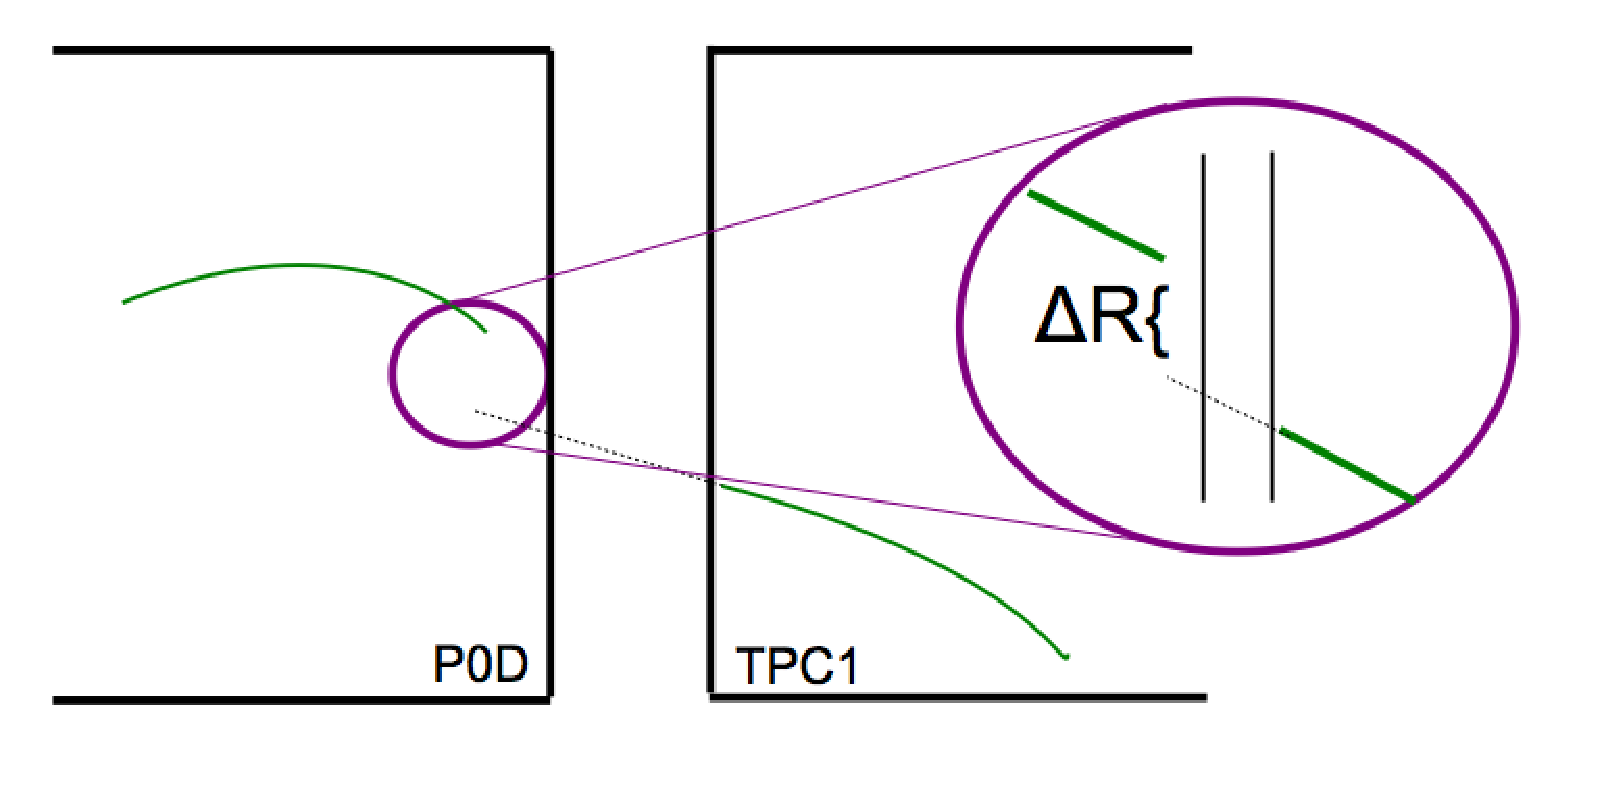
\includegraphics[width=3.2in]{Figures/drCalc.eps}
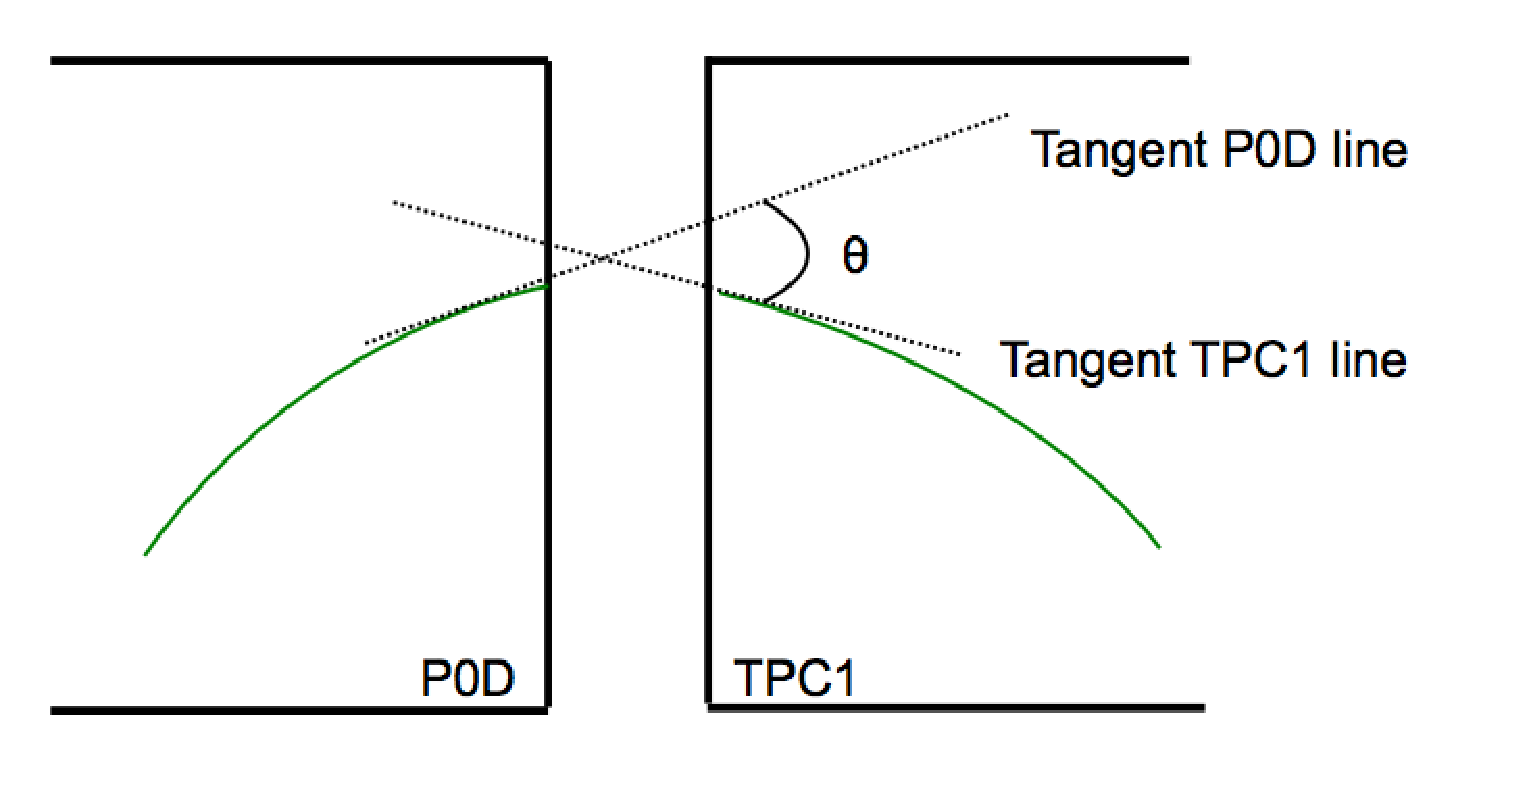
\includegraphics[width=3.2in]{Figures/sindThetaCalc.eps}
\end{center}
\caption{Graphic demonstrating how the analysis calculates $\Delta R$ (left) and sin($\Delta \theta$) (right) for the track matching algorithm.}
\label{fig:dRCalc}
\end{figure}

We use a simple figure of merit (FOM) optimization process on beam MC to determine the cut values of $\Delta$R and sin$\Delta\theta$. The chosen FOM is 
\begin{equation}
F = \frac{\delta S}{S} = \frac{\sqrt{S+2B}}{S}
\end{equation}
\noindent where S is the total number of signal events passing a certain ($\Delta$R, sin$\Delta\theta$) cut, B is the background and $\delta S$ is the error. The second form of the FOM comes from assuming poissonian errors on the total number of events and the number of background events B. Minimizing this figure of merit will maximize the total signal while minimizing the error on the signal. We use beam MC and follow the matching procedure described above up to the  ($\Delta$R, sin$\Delta\theta$) cut. For every pair of  ($\Delta$R, sin$\Delta\theta$) cut values, the signal is defined as the number of successfully matched tracks that have both track segments originating from the same primary true trajectory (a primary trajectory is a true particle vector leaving the original vertex). Then the background is the remainder of the tracks that were matched but were not from the same primary trajectory. A 3D FOM histogram is created (see Figures \ref{fig:FOM1} and \ref{fig:FOM2}) where each bin (i,j) is filled with the calculated FOM from the matching algorithm with cuts $\Delta$R$\leq$i and sin$\Delta\theta\leq$j. 

\begin{figure}
\begin{center}
\includegraphics[width=6in]{Figures/FOM1.png}
\end{center}
\caption{The figure of merit value as a function of $\Delta$R and sin$\Delta\theta$ cut values using run 2 water-in MC. The left side shows the entire allowed cut region and the right side is zoomed in to the local maximum (76~mm, 0.88) with the Z axis zero suppressed.}
\label{fig:FOM1}
\end{figure}

\begin{figure}
\begin{center}
\includegraphics[width=6in]{Figures/FOM2.png}
\end{center}
\caption{The figure of merit value as a function of $\Delta$R and sin$\Delta\theta$ cut values using run 3 water-out MC. The left side shows the entire allowed cut region and the right side is zoomed in to the local maximum (78~mm, 0.90) with the Z axis zero suppressed.}
\label{fig:FOM2}
\end{figure}

The FOM does not vary wildly over the scanned cut values. In fact, we have to zoom into the optimal region to even see where the local maxima is located. These maxima are shown in the right hand histogram in Figures \ref{fig:FOM1} and \ref{fig:FOM2}. They are at the coordinates (76~mm, 0.88) and (78~mm, 0.90) for water-in and water-out samples respectively. To simplify the selection procedure, we use the more stringent of the two cut choices, specifically $\Delta$R $\leq$ 76~mm and sin$\Delta\theta\leq0.88$ for all data and MC samples. Finally, we also investigate the agreement between data and MC in the distributions of the matching parameters. Large differences in the $\Delta$R and sin$\Delta\theta$ distributions of data and MC would cause a systematic difference in our data and MC selection efficiencies. This effect is accounted for by detailed systematic studies on the matching efficiency conducted in Section \ref{sec:matchingsyst}, but we also show in Figures \ref{fig:matchpar1} and \ref{fig:matchpar2} that the pre-cut data and MC distributions of $\Delta$R and sin$\Delta\theta$ track each other quite well near the cut values. Note that as the MC we use does not simulate external interactions, we apply a loose vertex position cut ($Z>$ -3183~mm, $|X|$ and $|Y|<$ 1000~mm) on the data.

\begin{figure}
\begin{center}[h]
\includegraphics[width=6in]{Figures/matchpar1.png}
\end{center}
\caption{The pre-cut $\Delta$R (left) and sin$\Delta\theta$ (right) distributions for data (black) and MC (red) using run 2 water-in samples.}
\label{fig:matchpar1}
\end{figure}

\begin{figure}[h]
\begin{center}
\includegraphics[width=6in]{Figures/matchpar2.png}
\end{center}
\caption{The pre-cut $\Delta$R (left) and sin$\Delta\theta$ (right) distributions for data (black) and MC (red) using run 3 water-out samples.}
\label{fig:matchpar2}
\end{figure}

\subsection{Track Momentum Reconstruction}
\label{sec:momrecon}

To reconstruct the momentum of the muon track, we use the momentum measurement from TPC1 made by fitting a helix to the track and comparing the curvature to the local magnetic field. This momentum is then corrected for the segment of the track that passed through the P0D. Using muon range tables in conjunction with the known materials density in the different P0D regions, we can calculate the momentum of the muon at the vertex by adding in the total energy lost. As we must do this for every single muon-like negative track in every event, we require that the algorithm is fast. So we chose not to use $\frac{dE}{dx}$ tables to incrementally restore the energy lost. Instead, the P0D energy loss was calculated using range data for the two types of superP0Dules: water target and ECAL. Range is defined as
\begin{equation}
R(E') = \int^{E'}_{0} \left(\frac{dE}{dx}\right)^{-1} dE
\end{equation}
where $\frac{dE}{dx}$ is the weighted average energy loss over all materials. The range is calculated for each superP0Dule. This gives us a table of range vs energy/momentum for each section of the P0D and avoids performing the integration every single time a track is found. The track length in the P0D is used to find the corresponding energy lost (see Figure \ref{fig:eloss}) and add it to the TPC1 measurement momentum. If the track traversed through mutiple superP0Dules, as it must, then the energy loss look-up procedure is performed separately for each. The momentum residual as defined by $(P_{reco}-P_{truth})/P_{truth}$ for run 2 water-in and run 3 water-out samples is shown in Figure \ref{fig:momres} for reference. The algorithm does an excellent, unbiased job of reconstructing muon momenta according to MC.

\begin{figure}
\centering
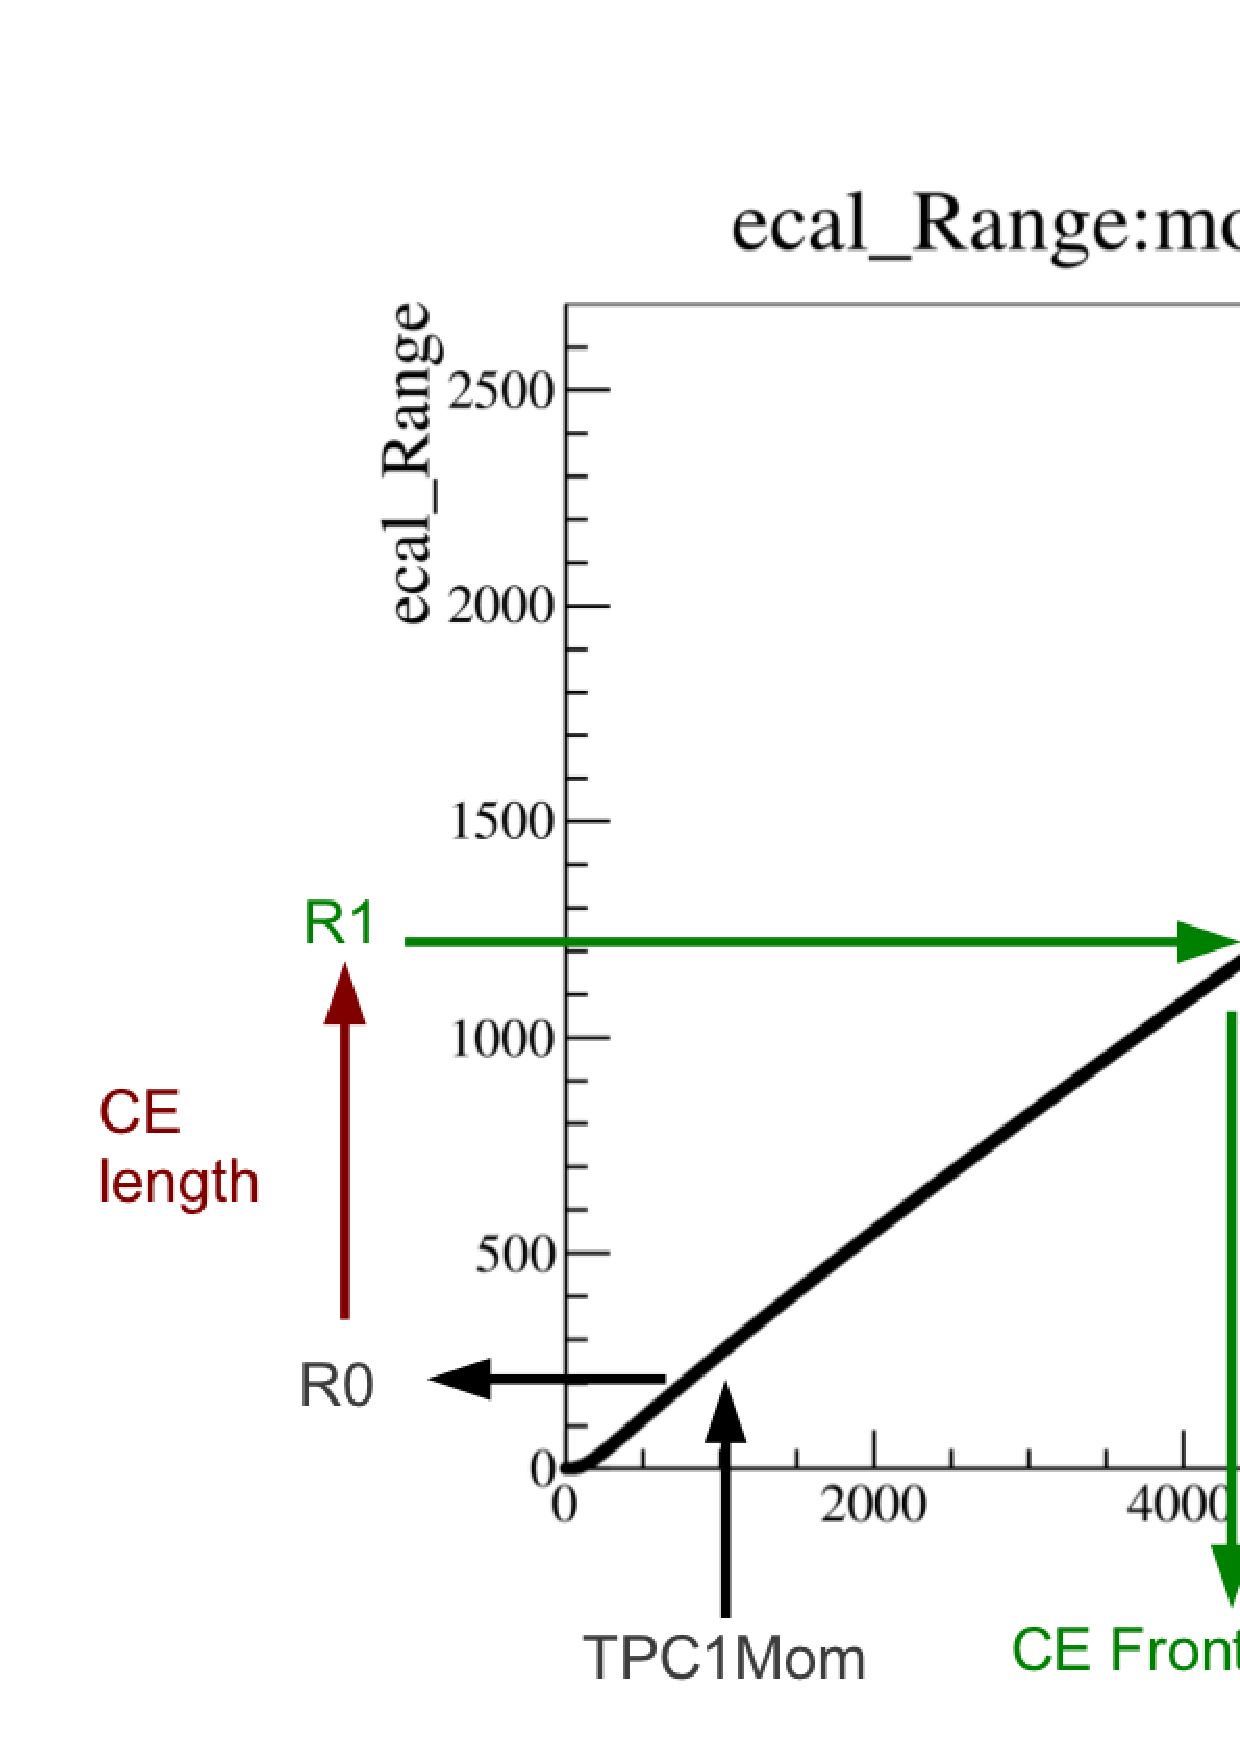
\includegraphics[width=5.5in]{Figures/eLossCalc1.png}
\caption{Calculation of P0D momentum correction. The steps of the correction
are shown schematically with the arrows} 
\label{fig:eloss}
\end{figure}

\begin{figure}
\centering
\includegraphics[width=5.5in]{Figures/momentumresidual.png}
\caption{The momentum residual comparing the reconstructed momentum with the true track momentum in run 2 water-in MC (blue) and run 3 water-out MC (purple).}
\label{fig:momres}
\end{figure}

\clearpage
%\clearpage
\section{Inclusive Charge Current event selection}
\label{sec:InclusiveSelection}

The muon neutrino beam produced at J-PARC passes through the 
off-axis ND280 detector. 
These neutrinos can have Charged Current (CC) 
or Neutral Current interactions with the detector material. 
The CC interactions are expected to produce a $\mu^-$ track
and these $\mu^-$ tracks usually contain  most of 
the momentum from the incident neutrino.
Therefore we search for the highest momentum negative track 
which simplifies the identification and tagging of  
a CC interaction event candidate. %\\
%It is important to note that 
We note that 
the beam spill delivered by J-PARC 
to the experiment has a sub-structure of bunches which are 
separated by beam dead-time. 
All analyses described in this document were done 
at the bunch level instead of the ND280-DAQ event level (Spill level).\\
hjbvjvjv

The selection procedure includes 
the three main information levels 
and 
%. The selection flow 
is listed below:
%includes three steps that correspond
%to the three information levels, (that follow each other) 
%which are
\begin{itemize}
\item 
Beam and Data Quality information:\\
Each Spill is checked to have
\begin{itemize}
\item 
Beam Data flag: `GoodSpillFlag' set to the value of one
\item
Data Quality flag: `ND280OffFlag' equal to zero
\end{itemize}
\item 
Individual global track information: \\
Each track in a good spill is required to have 
\begin{itemize}
\item
The `Status' flag not set to zero
\item
The `FrontMomentum' property %!= 10,000 
not equal to the default value of 10,000
\item
 Its start position (`FrontPosition') 
inside the analysis~\p0d~Fiducial~Volume 
\item
Measured information from TPC1 sub-detector
\end{itemize}

\item 
Bunch time window information: \\
At this stage the tracks are sorted into predefined bunch time windows 

\begin{itemize}
\item
In each bunch window we tag the highest momentum negative track 
as our candidate track
\end{itemize}

\end{itemize}

The next subsections will describe in detail both 
the Fiducial Volume (FV) determination procedure 
and the setup of the time windows that were used in the analyses.


%The tagged events from these selection procedure would be used 
%
%The first step verifies that we have good beam data 
%as well as good ND280 Data Quality (DQ) data.
%The second step includes checks 
%on each of the recorded global tracks. These involved 
%test of the track Status property as will as to reject 
%tracks with the default the momentum 10,000. After that 
%the start position of each track is exam 
%to be in the defined \p0d Fiducial Volume (FV) 
%and was verified to contain  measured information 
%from TPC1 sub-detector.
%In the last step, the tracks are sorted into (predefined) 
%specific bunch time windows 
%and the highest momentum negative track of each is tagged 
%as the candidate track.

\subsection{Fiducial Volumes Determinations}

The fiducial volume determination is an important step 
in the selection procedure. 
It is the main step that reduces most of the background 
while retaining signal events in 
the analysis. \\

The method adopted here involved the optimization of the expression 
\begin{equation}
\frac{\delta N_s}{N_s}
=\frac{\sqrt{(\delta N_{total})^2+(\delta N_{bg})^2}}{N_s}
=\frac{\sqrt{N_{total}+N_{bg}}}{N_s}
\label{eq:fiducialOptomize}
\end{equation}
were $N_s$ ($N_{bg}$) is the number of signal (background) events 
and the total number of events is $N_{total}=N_s+N_{bg}$. \\

The sideband samples that were chosen for this  
optimized minimization procedure 
were the one track reconstructed MC spills, 
where one can retrieve the NEUT generator truth information 
to assist in the determination of 
a fiducial ``signal" or a ``background" event. 
We note that for the Run 2 studies we used the samples 
that correspond to the case where the \p0d water bags 
were filled.\\

The optimization process was done for one boundary at a time
while the other boundaries were kept at a constant value. 
These initial constant values were fixed to be 
within the \p0d detector,  
namely $\pm 800\ {\rm mm}$ for both X and Y axes and 
$-3300 < Z < -970\ {\rm mm}$ for the third axis. 
The optimization scan procedure started with the X axis followed 
by the Y axis and ended with the Z axis. 
At the end of the optimization process, 
an additional fiducial scan was done for the X axis 
which confirmed that the yielded values are convergent. \\

The first step of the scanning procedure was to set a FV. 
In the next step only reconstructed tracks 
which had their start position inside that volume
were %considered/tested/
examined.
%The optimized boundary scan used only the reconstructed tracks 
%that started within the scanned FV region.
%Therefore as the scan progress into the \p0d volume the 
%number of total tracks considered dropped. 
%For boundary scan the only track considered are the ones that start 
%in the excact FV that is scanned. 
The following %(followed) 
step labeled a track as 'signal' 
if a true vertex was found in the same scanned FV 
and its truth 
ReactionCode\footnote{NEUT ReactionCodes 1$\rightarrow 26$} 
was consistent with a CC interaction.
All other tracks were labeled as `background'. \\

We took into consideration three points 
in the fiducial boundaries study.
\begin{itemize}
\item 
%1) The MC samples we used does not incorporate the exact water level 
The \p0d water levels set in the MC samples do not correspond 
to the actual levels measured in both runs. 
Therefore the positive Y axis boundary needs to 
be extracted from these water level measurements with 
an additional safety margin to ensure that all bags are filled with water.
\item 
The Z axis boundaries that are upstream of the face of a 
\p0dule are ignored. Therefore after the Z axis scan 
these boundaries are set to the upstream face value of 
the next inner \p0dule.
\item 
Since the \p0d reconstruction algorithm uses at least three 
\p0dules to extract a track in the \p0d, 
the maximum Z boundaries are set to the upstream face 
of the second to the last \p0dule (z = $-1010\ {\rm mm}$).

\end{itemize}

%From the fact that our 
The current MC samples that were used do not 
%contain or %(nor) 
simulate all possible neutrino interactions 
%these samples 
and therefore they lack additional sources of contamination,
i.e. rock muons or other neutron sources that are present in our data samples.
%Therefore the FV values that we will retrive from these MC samples 
%do not take into account 
To improve and try to bridge this deficiency we have decided to 
extend our fiducial scan with 
the additional information recorded in the data samples. 
This extension assumes that our signal is described 
to the best of our knowledge by the MC simulation and that 
all extra excess in data is assigned to be fiducial ``background"
(with the assumption that the majority of the difference between data 
and MC comes from rock muon-like sources). \\

\begin{figure}[!h]
\centering
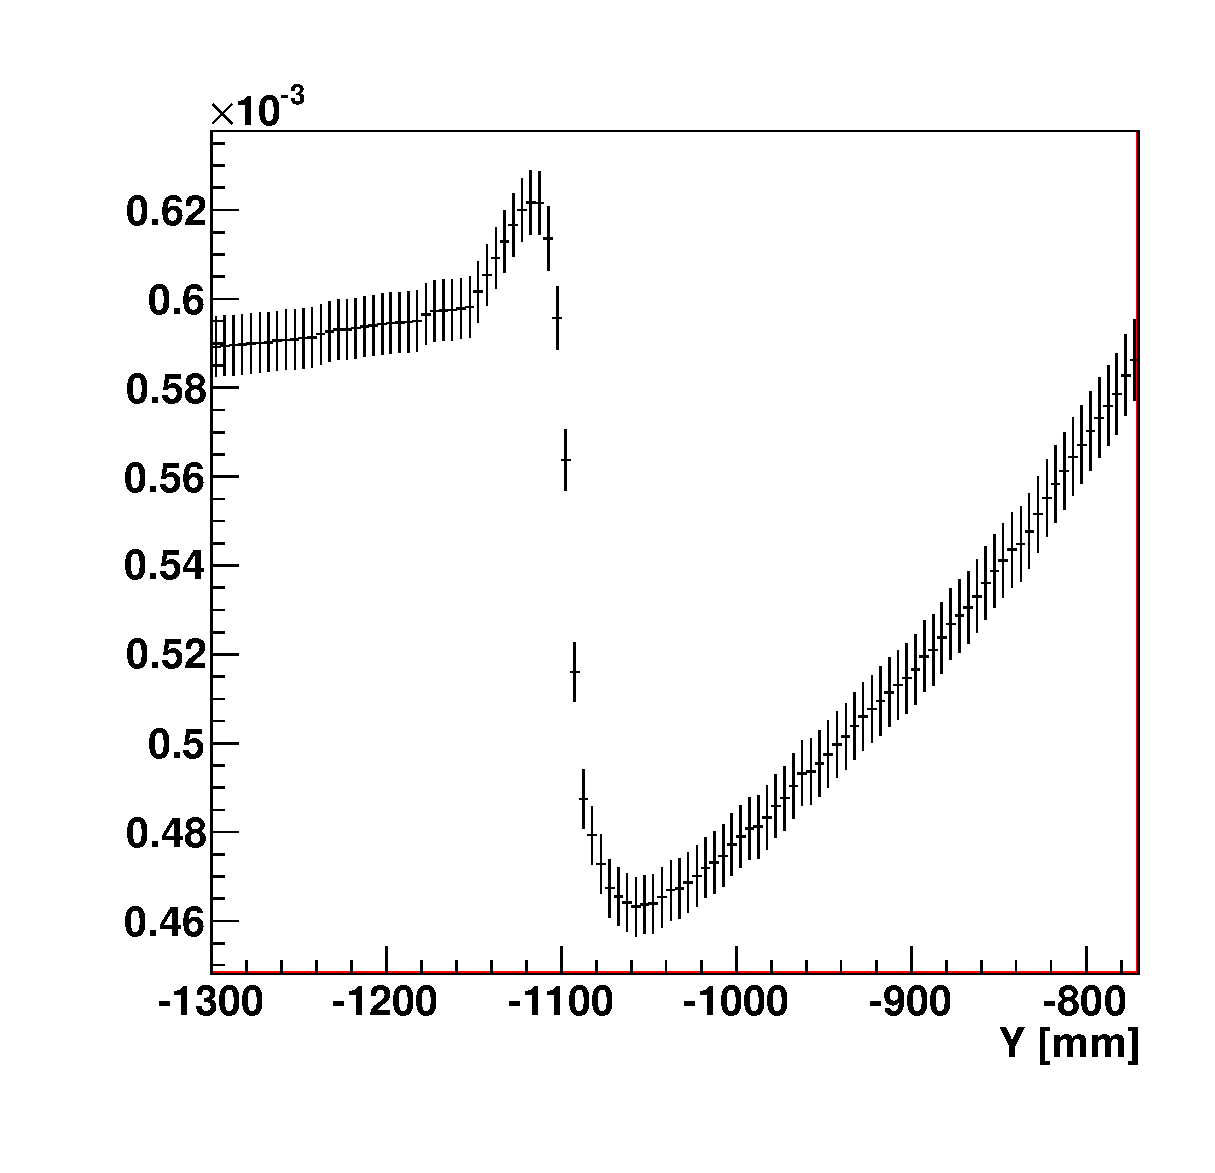
\includegraphics[width=3in]{Figures/FiducialScan-Run1-Yneg.eps}
\includegraphics[width=3in]{Figures/FiducialScan-Run2-Xpos.eps}
\caption{Fiducial scan results calculated from 
Eq. \ref{eq:fiducialOptomize} as a function of a given boundary value. 
Left: The fiducial scan results for the negative Y axis boundary of Run 1. 
Right: The fiducial scan results for the positive X axis boundary of Run 2. 
}
\label{fig:fiducialScanResults}
\end{figure}

In practice 
both MC and data samples had the same reconstruction requirements 
of one track per spill that had its start position in the scanned FV. 
This requirement defined $N_{total}$ for both sample types. 
The signal definition was extracted directly from the MC sample 
normalized down by POT to the equivalent data sample. 
The background definition came from the subtraction 
of the MC normalized signal ($N_{s}$) from data $N_{total}$. 
These two definitions were used to calculate 
the value of Eq. (\ref{eq:fiducialOptomize}) for different 
FV boundaries. 
The outputs of these calculations could be used to identify 
the desired minimum values.
Two of the FV scan results are 
shown in Fig. \ref{fig:fiducialScanResults}. 
The figure presents the output results of the negative Y axis scan for Run 1 
and the positive X axis scan for Run 2.  \\

%\begin{figure}[h]
%\centering
%\includegraphics[width=3in]{Figures/triumf-Run1-water-NPIDs.eps}
%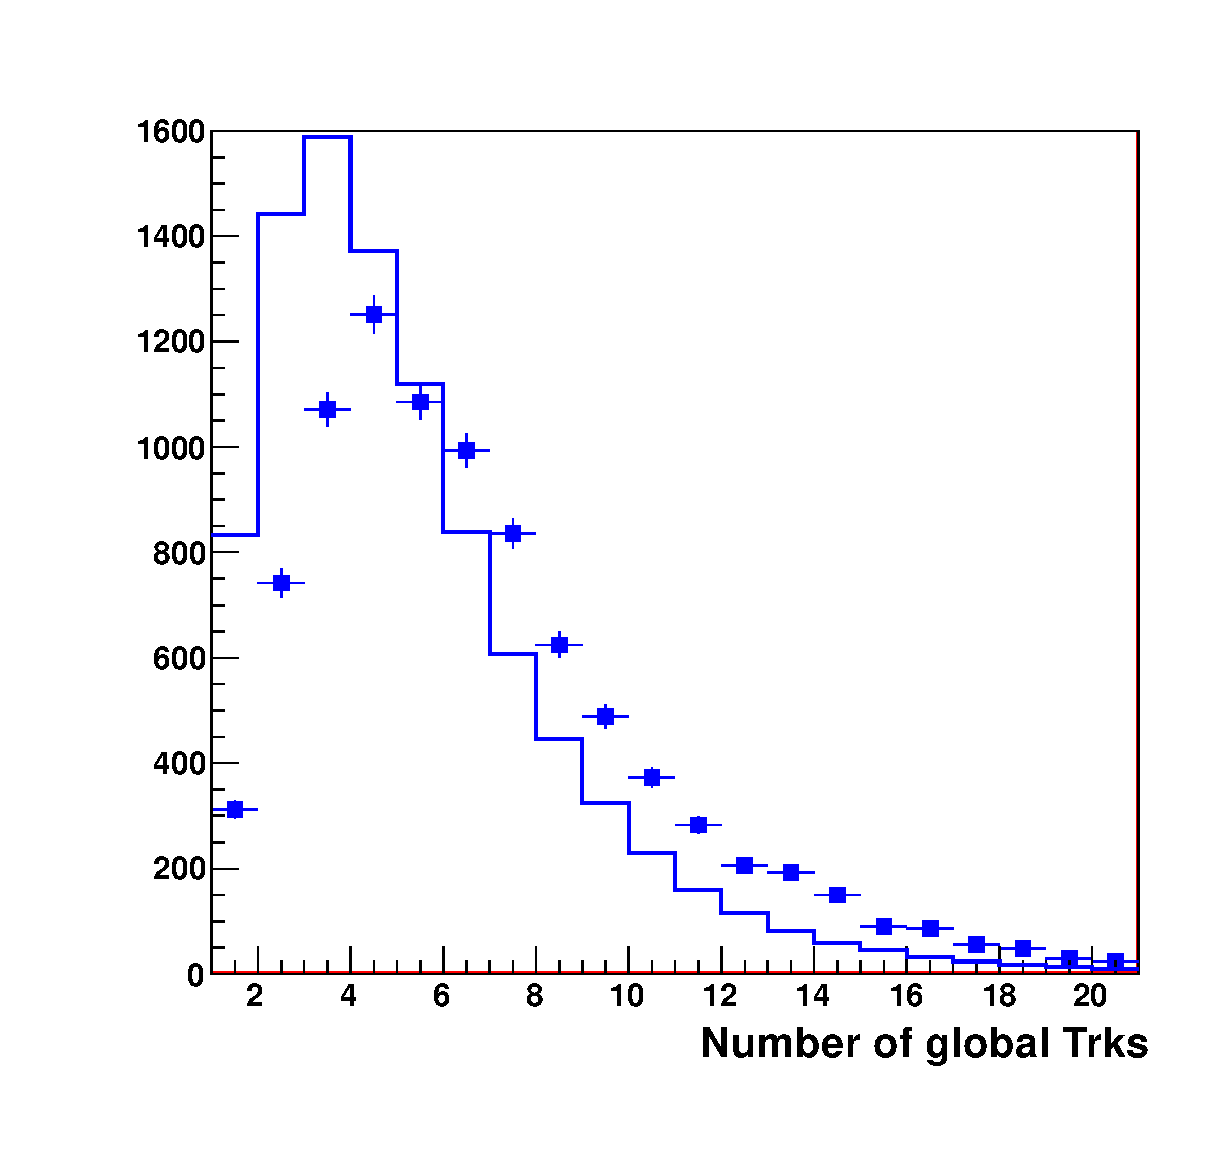
\includegraphics[width=3in]{Figures/triumf-Run2-water-NPIDs.eps}
%\caption{Number of global tracks: Data (points) and MC (Historgam). 
%On the Left (Right) Run 1 (Run2).}
%\label{fig:fiducialNPIDs}
%\end{figure}
\begin{table}
\centering
\begin{tabular}{ccccccc}
%\toprule
 & Run 1 & & & & Run 2 & \\
\cline{1-3}\cline{5-7}\\
Minimum [mm]& Axis & Maximum [mm] & & Minimum [mm]& Axis & Maximum [mm] \\
\cline{1-3}\cline{5-7}\\
-1020 & X & \ \ 990 &\ \ & -1030 & X & \ \ 970 \\
-1045 & Y & \ \ 850 & & -\ 950 & Y & \ \ 850 \\
-3175 & Z & -1010 & & -3175 & Z & -1010 \\
\cline{1-3}\cline{5-7}\\
%\hline\\
%\bottomrule
\end{tabular} 
\caption{The final FV boundaries for the different run periods.}
\label{tab:FV} %FIXME
\end{table}

The final FV boundaries, 
including the restrictions mentioned above, 
are summarized in Table \ref{tab:FV} for both T2K runs. 
A close look at the extracted values reveal that the 
boundaries are not so different between the two runs.

%\subsubsection{Additional checks/tests}
%
%We have issued additional checks on the FV values we extracted 
%with the use of the same sideband samples 
%this was due to possible concerns about \\


%Although we expect the ND280 fiducial cut to remove much of the background
%contribution from magnet interactions and sand muons, we still require a \p0d
%fiducial cut to select \p0d specific interactions. In the X and Y directions, the
%background is a combination of both magnet interactions and sand muons. Whereas
%in the Z direction, we expect a predominantly sand muon background.
%To first order, we have neglected to optimize the \p0d fiducial cut
%for purity and efficiency and instead chosen to cut out regions where a buildup
%of background events is evident. To this purpose, we used a large set of data to
%plot the X, Y and Z positions of the vertex of the highest momentum negative
%track in each event (no fiducial or other cuts were applied here).

%\begin{figure}
%\centering
%\includegraphics[width=5.5in]{Figures/vtxpos.eps}
%\caption{TO BE REMOVED OR REPLACED} 
%\label{fig:figA}%FIXME
%\end{figure}

\subsection{Bunch time windows}

We have studied the  track timing for Run 1 and Run 2
for both data and MC samples.
These studies have revealed a number of points that 
had to be addressed by our bunch time window determination 
and are listed here.
\begin{itemize}
\item
Run 1 has six bunches in each beam spill 
and Run 2 has eight bunches in each beam spill.
\item
Run 2 includes a bunch time shift that was introduced in January 2011.
\item
The MC sample has the same six/eight 
bunch structure as the data sample but the bunches 
are shifted on average by 82-96 ns from the data.
\end{itemize}

\begin{figure}
\centering
%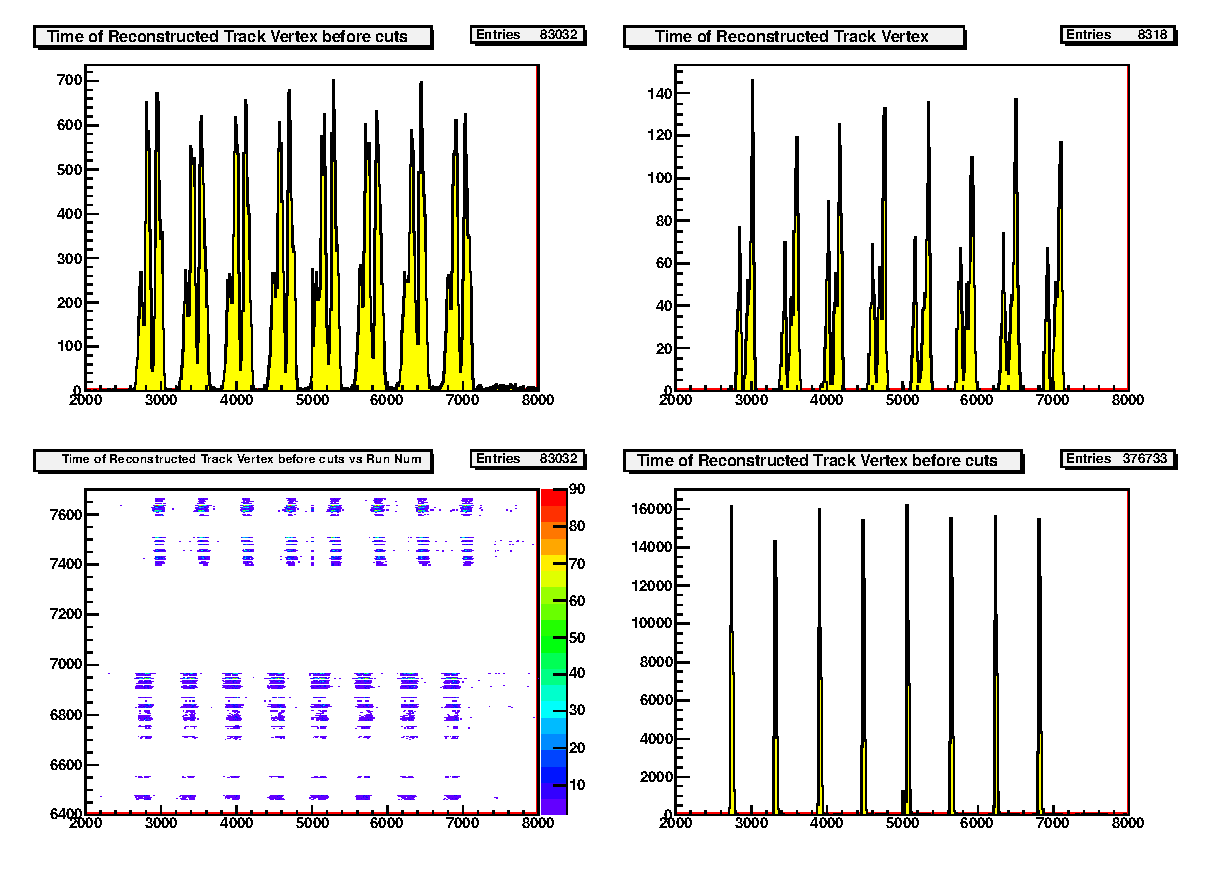
\includegraphics[width=0.95\textwidth]{Figures/BeamStructure.eps}
\includegraphics[width=4in]{Figures/spinD-TimeInSpill.eps}
\caption{Track timing as a function of SubRun for the data samples. 
The vertical dash 
line was added to guide the eye on the time shift that was introduced 
in Jan 2011.}
\label{fig:TrackTime}
\end{figure}

In Fig. \ref{fig:TrackTime}, 
which presents the track times 
as a function of their subrun for the data samples, 
one can observe some of these effects. 
A close examination of the figure shows both bunch structures 
and the time shift introduced in Jan 2011. a vertical dash line was added to guide the reader to see this relative shift. \\

%Fitting a gaussian to each of the time peaks, we find the location of the mean
%and determine an acceptable timing window. The same timing windows were used 
%for Run 1 and the two
%different time periods of Run 2. These are given below.

To account for the above conditions, we have decided to define 
the same set of bunch time windows for both runs.  The windows were enlarged to include both the difference between 
data and MC bunch means and the time shift in Run 2. 
Table \ref{tab:BunchTimeWindows} summarizes the 
bunch time windows used in the analyses. 

\begin{table}
\centering
\begin{tabular}{cc}\toprule
Bunch Number & Time window [ns]\\
\hline
 1 & 2700 - 3100\\ 
 2 & 3280 - 3680\\ 
 3 & 3860 - 4260\\ 
 4 & 4440 - 4840\\ 
 5 & 5020 - 5420\\ 
 6 & 5600 - 6000\\ 
 7 & 6180 - 6580\\ 
 8 & 6760 - 7160\\ 
\bottomrule
\end{tabular} 
\caption{The bunch timing windows used in the analysis 
for both Run 1 and Run 2.}
\label{tab:BunchTimeWindows} 
\end{table}



\section{Inclusive Charged Current Event Analysis}
\label{sec:InclusiveAnalysis}

The muon neutrino beam produced at J-PARC passes through the 
off-axis ND280 detector. 
These neutrinos can interact via Charged Current (CC) 
or Neutral Current with the detector material. 
The CC interactions 
%are expected to 
will 
produce a $\mu^-$ track 
which will contain most of the time the majority of 
the incident neutrino momentum. \\
The analyses strategy is to search for 
the highest momentum negative track in an event 
and to tag it as the muom candidate track and the while  
%tag the 
event as 
%which simplifies the identification and tagging of  
a CC interaction one.
We note that 
the beam spill delivered by the J-PARC facility  
to the experiment has a sub-structure of bunches which are 
separated by beam dead-time. 
All analyses described in this document were done 
at the beam bunch level instead of the ND280-DAQ event (beam spill level).

\subsection{Event Selection}
\label{sec:SelectionFlow}

The CC inclusive selection procedure includes the main levels of 
information available (accelerator/near-complex level, 
track level, bunch level) 
which 
%includes three main steps that
are listed below:
\begin{itemize}
\item 
%Beam and Data Quality selection cuts:\\
%Each Spill quality is checked to have both quality:
Accelerator/Near-Complex level selection:\\
A spill is use for analysis only if the below quality checks are satisfied
\begin{itemize}
\item 
The beam/accelerator flag `GoodSpillFlag' is set to the value one
\item
The near detector-complex Data-Quality flag `ND280OffFlag' is equals to zero
\end{itemize}
\item 
%Track level selection cuts: \\
Track level selection: \\
The Tracker-to-\p0d matching algorithm, which is outlined 
in Sec. \ref{sec:MatchingAlgorithm}, is applied. 

The algorithm inputs are the available \p0d and Tracker tracks in a spill 
and its outputs are a set of 
%all the 
tracks that originate in the \p0d \footnote{These will include tracks that 
started at the edges of the \p0d i.e. passing through tracks.}
 and continued to pass through TPC1/Tracker sub-detector.

To note is that the algorithm will match uniquely any \p0d/Tracker track 
with the nearest Tracker/\p0d track 
(by $\Delta R$, see Sec. \ref{sec:MatchingAlgorithm}). 
%
%In each spill, we match together reconstructed tracks from TPC1/Tracker 
%and \p0d using the matching algorithm outlined in Section \ref{sec:MatchingAlgorithm}. As all of the track quality cuts have already been made at the matching stage, we only need a few more selection steps. These tracks must:

\item 
Bunch level selection:\\
All the output tracks from the previous stage are sorted into 
predefined bunch time windows (See Table \ref{tab:BunchTimeWindowsProd5}). 

Then from each active bunch we identify the muon candidate track 
and tag that event as a CC interaction.

A track is considered as the muon candidate if it satisfied 
all the requirements below.

\begin{itemize}
\item 
The candidate track charge is negative \\
(by the matched Tracker track charge property).
\item 
The candidate track begins in the \p0d volume\\ 
($-988\ mm< X <910\ mm$, $-1020\ mm< X <1010\ mm$, $-3139\ mm< X <-900\ mm$). 
This condition is required to reject external sources tracks   
(cosmic, magnet or sand interactions) while keeping the largest 
volume of the \p0d detector as a target. 
\item 
The candidate track momentum at the start of the track is the highest 
in that bunch.
\end{itemize}

%Then in final step the algorithm identifies in each bunch the highest momentum 
%candidate pair track and tags it as the muon candidate.
Finlay, only the muon candidate tracks which originated from 
inside the \p0d Water-Target FV (see Sec. \ref{sec:WTFV}) 
are accounted for the final results. 
\end{itemize}

\subsubsection{The \p0d Water Target Fiducial Volume}
\label{sec:WTFV}

The Water-Target (WT) Fiducial Volume (FV) cut used in this document  
is based on the FV description given in T2K-TN-073. 
The choice of the FV in the X and Y directions 
is made to minimize the uncertainty of the amount of water in the \p0d. 
In the Z direction, the FV corresponds to the water target region only. 
This also minimizes the physics uncertainty arising from 
the lead radiator sheets in the ECal super-\p0dules that 
are on the upstream and downstream ends of the water target. 
The FV values utilized in this note are summarized in Table \ref{tab:WTFV}.

\begin{table}[h]
\centering
\begin{tabular}{ccccc}
\toprule
Minimum & & & & Maximum \\
\hline
 -836 & $<$ & X & $<$ & 764 \\
 -871 & $<$ & Y & $<$ & 869 \\
 -2969 & $<$ & Z & $<$ & -1264 \\
\bottomrule
\end{tabular} 
\caption{The \p0d Water-Target Fiducial Volume used in the analyses, 
taken from Ref. \cite{tn73}}
\label{tab:WTFV} 
\end{table}

\subsubsection{Bunch Time Windows}
\label{sec:BunchTimeWindow}

%As 
The beam spill substructure is not the same for the different 
beam run periods, we have studied the track timing 
for Run 1-4 % and Run 2
for both Data and MC samples.
These studies have revealed a number of points that 
had to be addressed by our bunch time window determination 
and are listed here.
\begin{itemize}
\item
Run 1 has six bunches in each beam spill 
while Run 2 - 4 have eight bunches in each beam spill.
\item
Run 2 includes a bunch time shift that was introduced at January 2011 
(see Fig. \ref{fig:TrackTime}).
\item
The MC samples have the same six/eight 
bunch structure as the Data samples but their bunches (means) 
are shifted on average $\sim$250 ns from the data ones.
\end{itemize}

\begin{figure}
\centering
\includegraphics[width=4in]{Figures/spinD-TimeInSpill.eps}
\caption{Track time stamp as a function of subrun in Data 
(for Run 1 and Run 2 run periods). 
The vertical dash 
line was added to help point out the time shift that was introduced 
at Jan 2011.}
\label{fig:TrackTime}
\end{figure}

In Fig. \ref{fig:TrackTime}, 
which shows the track time stamps as a function of their subrun in Data, 
one can observe some of these effects mentioned above. 
A close examination of the figure shows 
both the six and the eight bunch structures 
and the time shift introduced at Jan 2011. 
A vertical dashed line was added to help the reader 
to help see this relative shift. \\

To account for the above conditions, we have decided to define 
the same set of bunch time windows for all runs periods 
(regardless of the run configuration).  
These windows were enlarged to include both the difference between 
Data and MC bunch means and the time shift in Run 2. 
Table \ref{tab:BunchTimeWindowsProd5} summarizes the 
bunch time windows used in the analyses. 

\begin{table}
\centering
\begin{tabular}{cc}\toprule
Bunch Number & Time window [ns]\\
\hline
 1 & 2660 - 3100\\ 
 2 & 3240 - 3680\\ 
 3 & 3820 - 4260\\ 
 4 & 4400 - 4840\\ 
 5 & 4980 - 5420\\ 
 6 & 5580 - 6000\\ 
 7 & 6140 - 6580\\ 
 8 & 6720 - 7160\\ 
\bottomrule
\end{tabular} 
\caption{The bunch timing windows used in the analyses 
for all Run periods.}
\label{tab:BunchTimeWindowsProd5} 
\end{table}

\clearpage

\subsection{Distributions and Selection Results}

In this section we present comparisons between data and Monte Carlo
for timing distributions, vertex distributions, momenta, $\theta$, and $\phi$. 
The Monte Carlo was reweighted to the 11b version 3.2 flux. The stacked color histograms in the following plots represent the MC distributions separated into different classifications. The color scheme used is shown in Figure \ref{fig:colorlegend}. Note that Quasi-elastic (QE), Single pion (Pi), Multi Pion (NPi), Meson, and Deep Inelastic Scattering (DIS) are all charged current interactions and are considered as signal in this analysis. Neutral Current (NC), parent Anti-Neutrino (antiNu), Other and Out of Fiducial Volume (outFV) interactions are all background.

\begin{figure}[here]
\centering
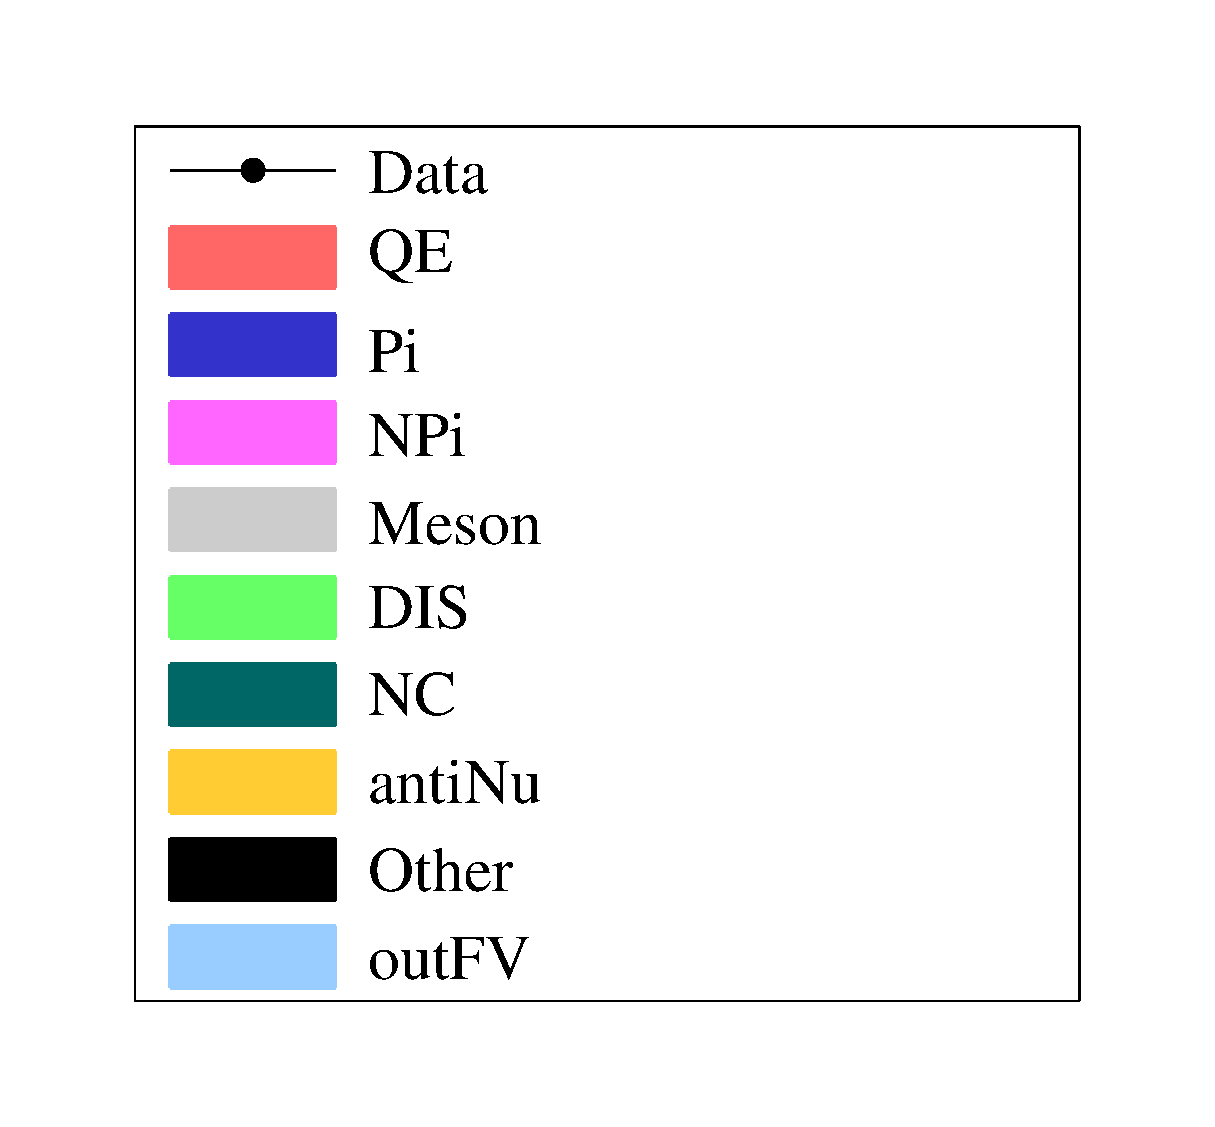
\includegraphics[width=3in]{Figures/Legend.eps}
\caption{The color scheme used for many of the Monte Carlo plots in the document. They are separated via NEUT reaction codes, parent neutrino flavor and vertex location. Refer to the text for further detail.}
\label{fig:colorlegend}
\end{figure}

\subsubsection{Timing distributions}

\begin{figure}[here]
\centering
\includegraphics[width=3in]{Figures/P0DTrkTimeRun1Run2Run4.eps}
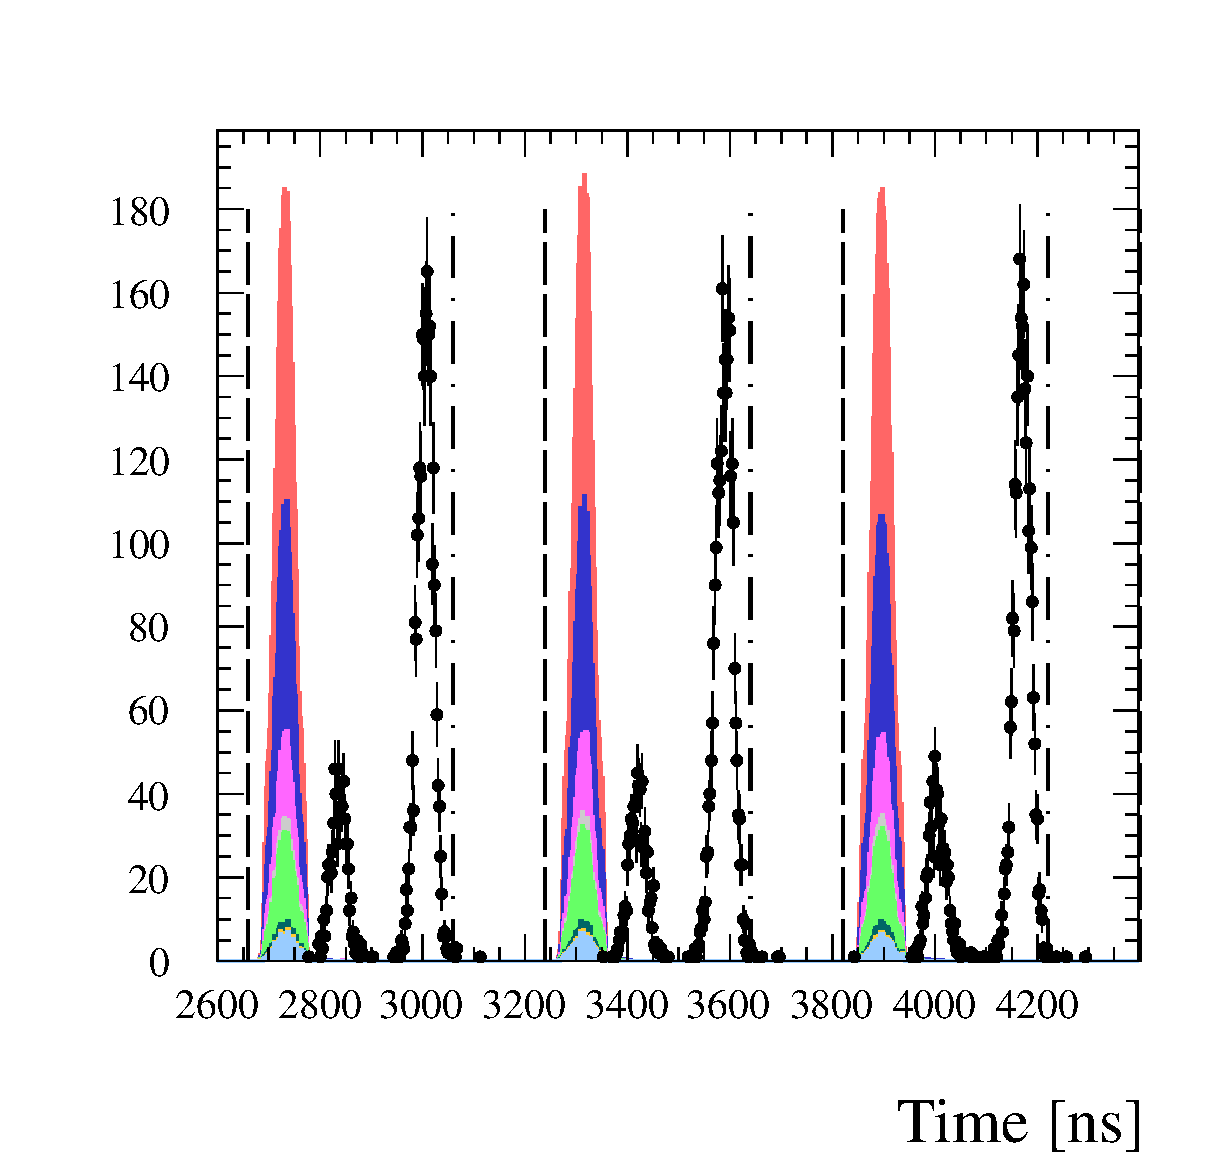
\includegraphics[width=3in]{Figures/P0DTrkTimeRun1Run2Run4-zoom.eps}
\caption{Time distribution of track vertices in Run 1 + Run 2 + Run 4. 
The MC is shown in color and the data in black crosses. 
The left plot shows all the beam bunches and the right plot show a zoom 
in of the first three beam bunches.}
\label{fig:run1time}
\end{figure}

The distribution of 'Water-in' track vertex time in Run 1, Run 2 and Run 4 
is shown in Figures \ref{fig:run1time}. 
We note that there is a discrepancy between the MC track time 
and the Data track time. 
Specifically, the peaks of MC and Data are shifted within the time window. 
%Also, the MC distribution shows a double peaked structure. These effects persist across both running periods with an added structure in the Run 2 data plot. Namely, we see thatin Run 2 there is a second peak in the track timing distribution of Data. 
These effects are not however much of an issue in our analyses as we have very lenient timing cuts. The relative position of peaks in a given time window has a negligible effect when we integrate over the entire window. Any effects at the edge of the timing cuts will be accounted for in our timing systematic.

\subsubsection{Vertex distributions}

We define the start position of the muon candidate track as the vertex. This start position is determined by \p0d reconstruction and corresponds to the first \p0dule to have an above-noise energy deposition from the charged track. For the Z-direction, this implies that the position can only be resolved up to the thickness of an individual \p0dule. The Z Vertex distributions have thus been binned by \p0dule thickness, a value that varies over the different super\p0dules. In the X and Y directions, though we can only get energy deposition in the discrete volumes of scintillator bars, the triangular shape of the bars allows most charged tracks to deposit energy into neighboring bars. The locations of these two hits and the amount of energy deposited at each can be averaged to give a more accurate measurement of where the track passed through the scintillator layer. Thus, the X and Y vertex positions can be resolved to a much higher precision than the Z position.

\begin{figure}
  \centering
  \includegraphics[width=3in]{Figures/P0DTrkXRun1Run2Run4.eps}
  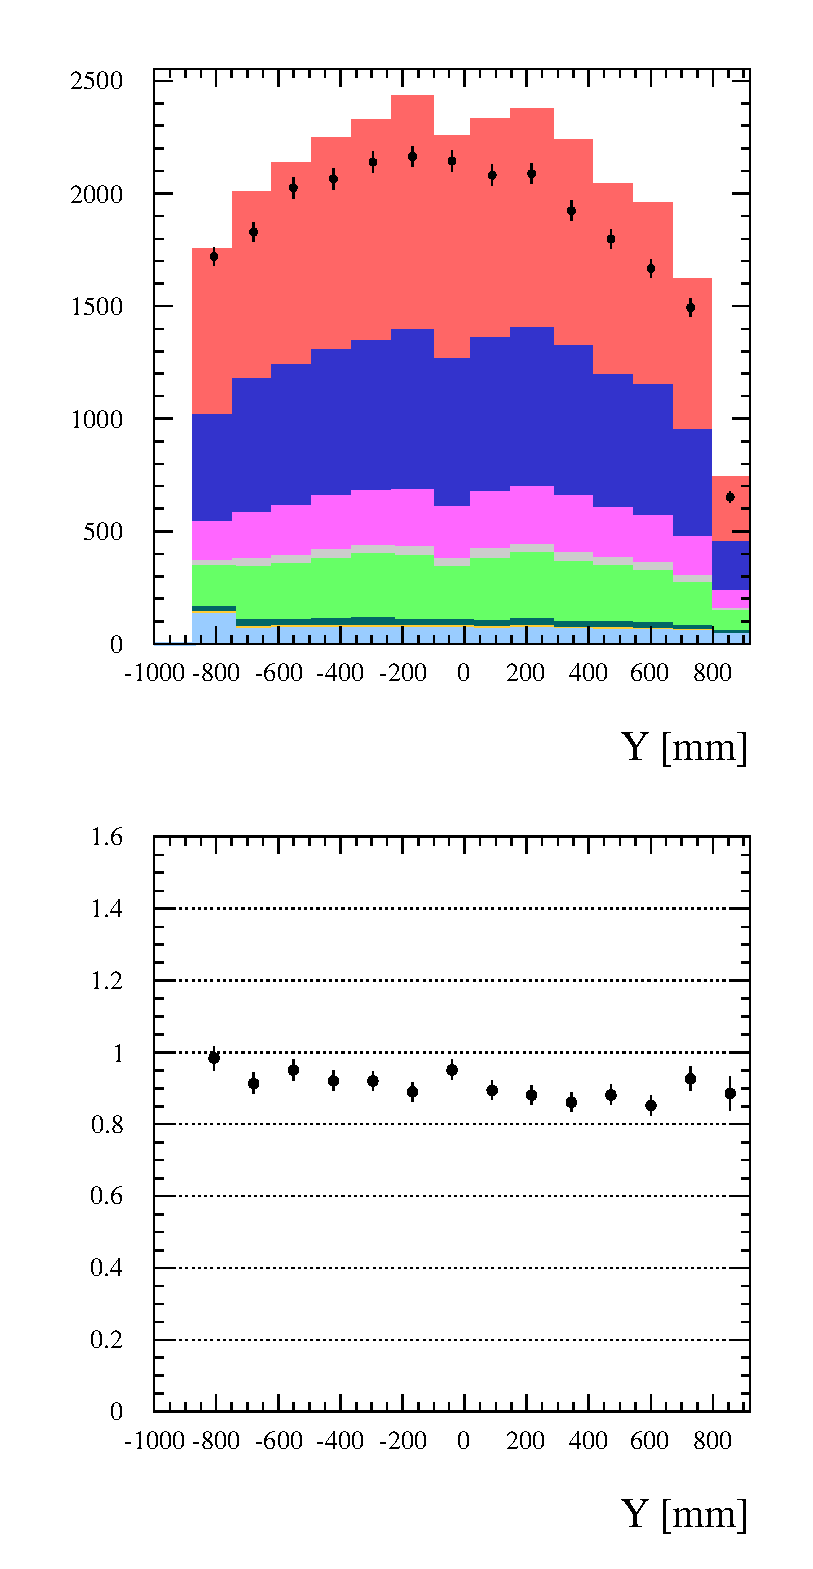
\includegraphics[width=3in]{Figures/P0DTrkYRun1Run2Run4.eps}
  \caption{The start position of the muon candidate track for 
Run 1, Run 2 and Run 4 'water-in' period. The X position (Y position) is shown to the left (right).
Below is the corresponding Data to MC ratio.} 
  \label{fig:XYRun1Run2Run4}%FIXME
\end{figure}

\begin{figure}
  \centering
  \includegraphics[width=3in]{Figures/P0DTrkXRun2airRun3airRun4air.eps}
  \includegraphics[width=3in]{Figures/P0DTrkYRun2airRun3airRun4air.eps}
  \caption{The start position of the muon candidate track for 
Run 2, Run 3 and Run 4 'Water-out' period. 
The X position (Y position) is shown to the left (right).
Below is the corresponding Data to MC ratio.} 
  \label{fig:XYRun2airRun3airRun4air}%FIXME
\end{figure}

The X, Y and Z vertex positions for the Run 1, Run 2 and Run 4 
'Water-in' periods are shown 
in Figures \ref{fig:XYRun1Run2Run4} and \ref{fig:ZRun1Run2Run4}. 
We note that the number of CC inclusive interactions increases 
as we go further downstream in the \p0d. 
This is an acceptance effect and is expected. 
The muon track candidate must enter the TPC. 
Tracks originating further upstream lose energy 
as they traverse the \p0d and so have  a lower chance of 
making it all the way to the TPC. 
Therefore we see the shape shown in the Z vertex distributions.

\begin{figure}
  \centering
  \includegraphics[width=4in]{Figures/P0DTrkZRun1Run2Run4.eps}
  \caption{The Z start position of the muon candidate track for 
Run 1, Run 2 and Run 4 'water-in' periods. 
The varying bin widths equal the thickness of a p0dule in that region. Below is the corresponding Data to MC ratio.} 
  \label{fig:ZRun1Run2Run4}%FIXME
\end{figure}

\begin{figure}
  \centering
  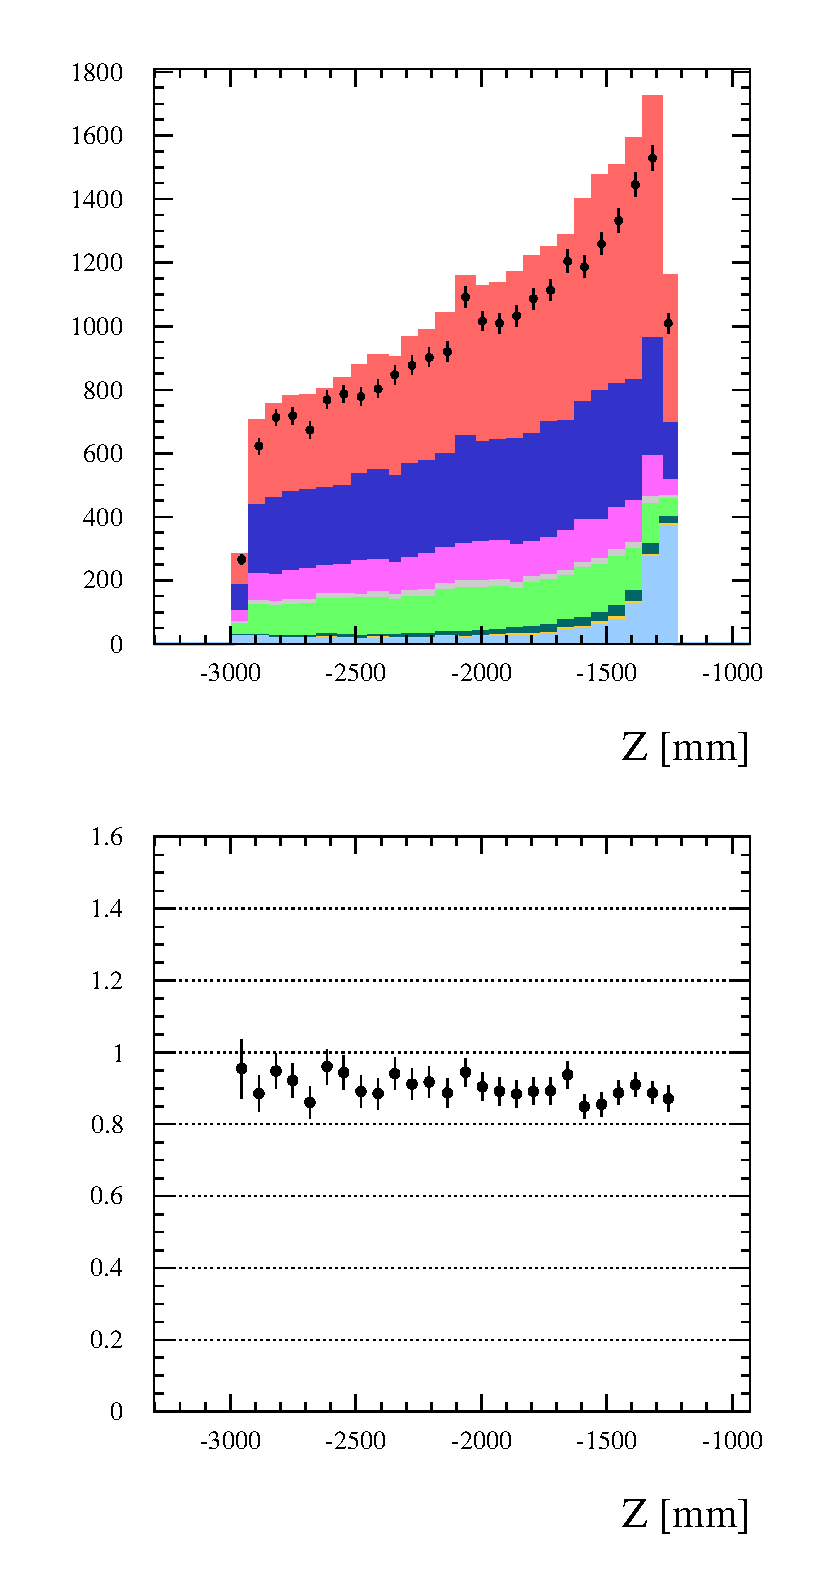
\includegraphics[width=4in]{Figures/P0DTrkZRun2airRun3airRun4air.eps}
  \caption{The Z start position of the muon candidate track for 
Run 2, Run 3 and Run 4 'Water-out' periods. 
The varying bin widths equal the thickness of a p0dule in that region. 
Below is the corresponding Data to MC ratio.} 
  \label{fig:ZRun2airRun3airRun4air}%FIXME
\end{figure}


\subsubsection{Kinematic Distributions}

We show here Data and Monte Carlo distributions of momentum, 
$\theta$ and $\phi$. 
The momentum distributions of the muon candidate tracks 
are shown in Fig. \ref{fig:PmuRun1Run2Run4} for Run 1, Run 2 and Run 4 
'Water-in' periods. 
The markers with error bars represent data with statistical errors 
and the colored histogram stack shows the Monte Carlo separated 
into different interaction categories. 
There is a qualitative agreement in the shape %and normalization 
of the overall momentum distributions between Data and Monte Carlo 
for Run1 + Run2.
 The majority of these background is in the lower momentum region. %Figure \ref{fig:PmuRun1Z} also shows the momentum distribution of the muon candidate track for Run 1 + Run2 respectively. The distributions are also divided into four plots corresponding to the four super\p0dules of the \p0d. The event rate, shape and low energy fall of all agree with what is expected once \p0d energy loss and track acceptance is accounted for.\\
We also show the $\theta$ and $\phi$ distributions of Data and Monte Carlo 
for both running periods. 
Figure \ref{fig:ThetaRun1Run2Run4} indicates that most of our tracks 
are forward going, significantly more so than the FGD selections. 
Once again, this acceptance effect is both expected due to the TPC1 segment 
requirement. 
Figure \ref{fig:ThetaRun1Run2Run4} shows the $\phi$ distribution 
for the combined running periods, and we note good agreement.

\begin{figure}
  \centering
  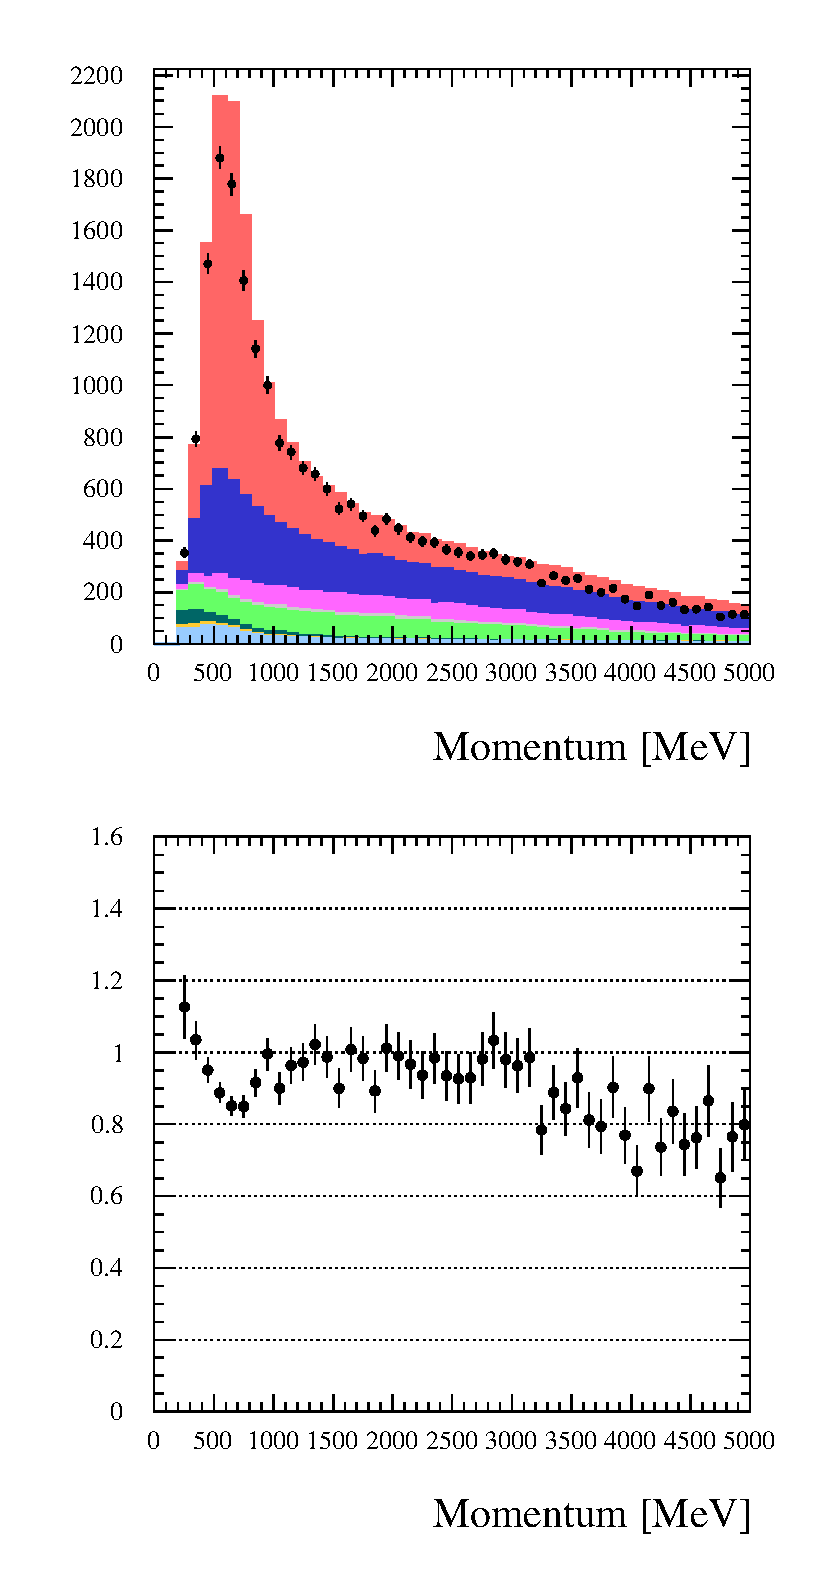
\includegraphics[width=4in]{Figures/P0DTrackerMomRun1Run2Run4.eps}
  \caption{The momentum at the vertex of the muon candidate for 
Run 1, Run 2 and Run 4 'Water-in' peridos. 
Below is the corresponding Data to MC ratio.} 
  \label{fig:PmuRun1Run2Run4}%FIXME
\end{figure}

\begin{figure}
  \centering
  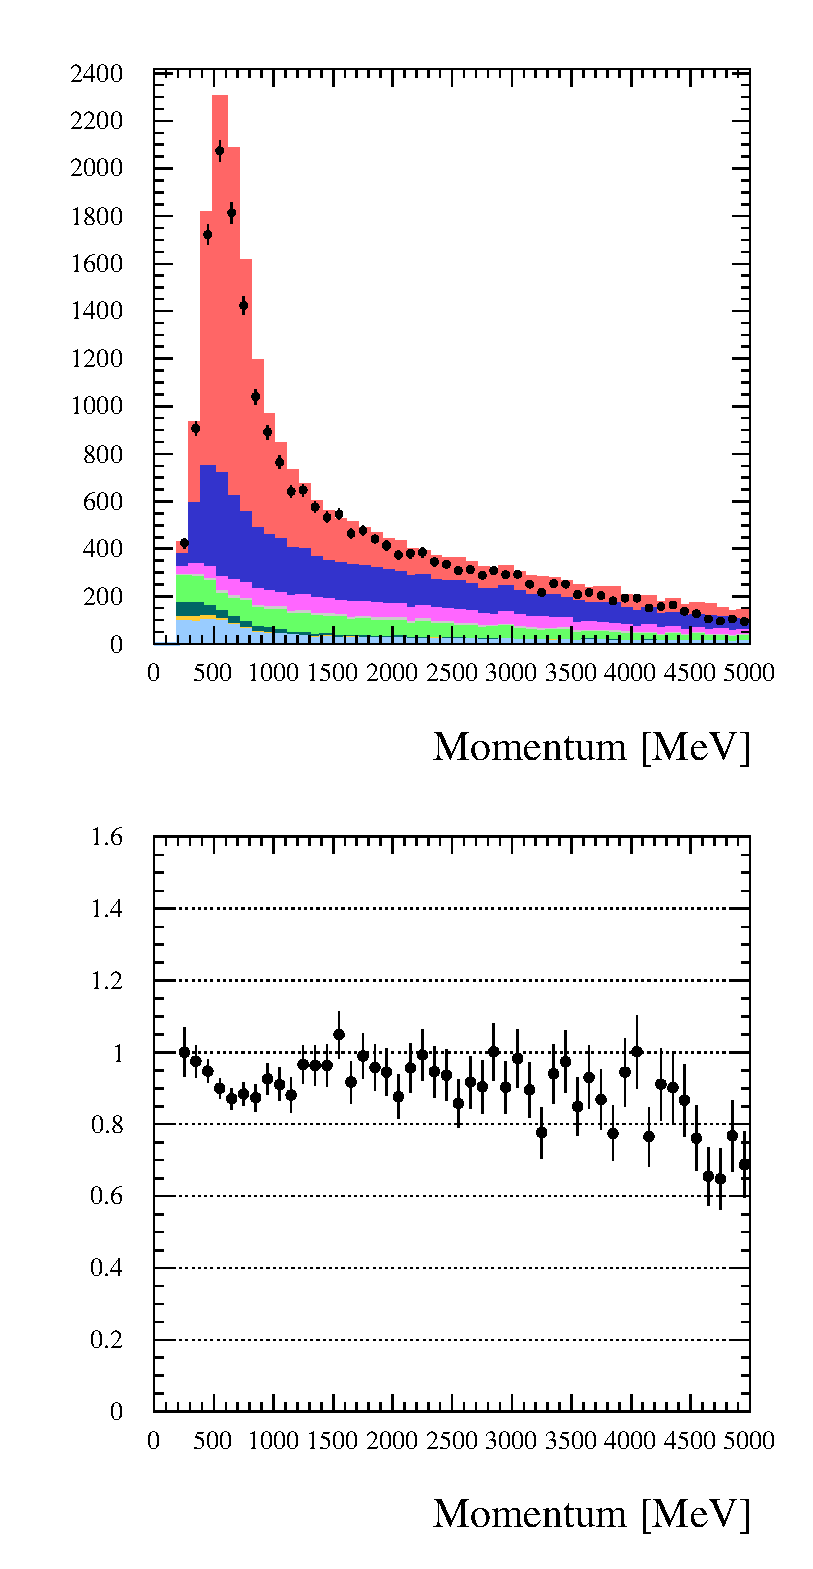
\includegraphics[width=4in]{Figures/P0DTrackerMomRun2airRun3airRun4air.eps}
  \caption{The momentum at the vertex of the muon candidate for 
Run 2, Run 3 and Run 4 'Water-out' peridos. 
Below is the corresponding Data to MC ratio.} 
  \label{fig:PmuRun1Run2Run4}%FIXME
\end{figure}

\begin{figure}
  \centering
  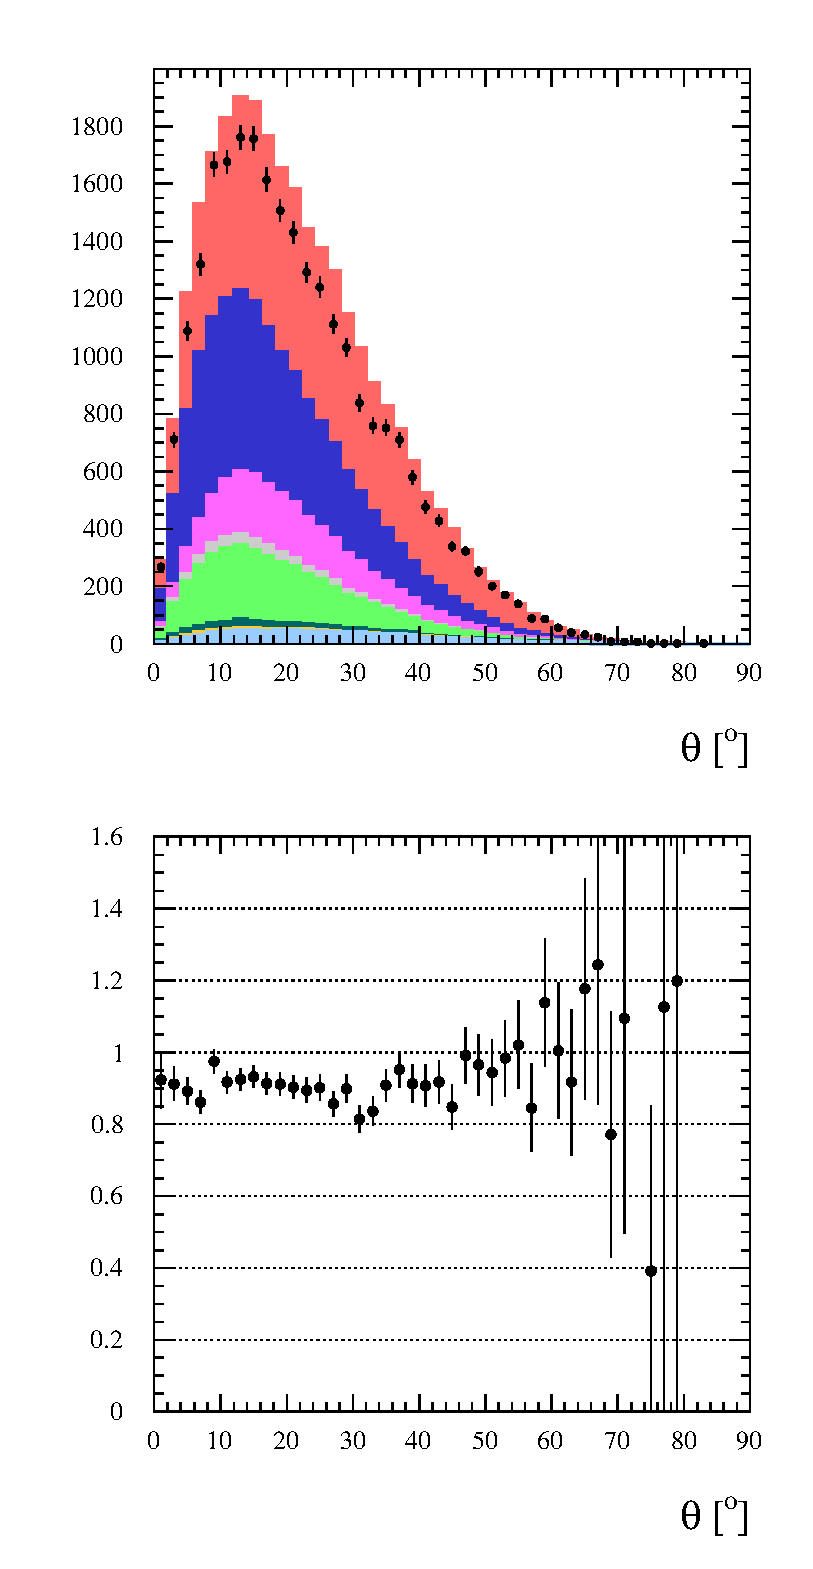
\includegraphics[width=3in]{Figures/P0DTrkThetaRun1Run2Run4.eps}
  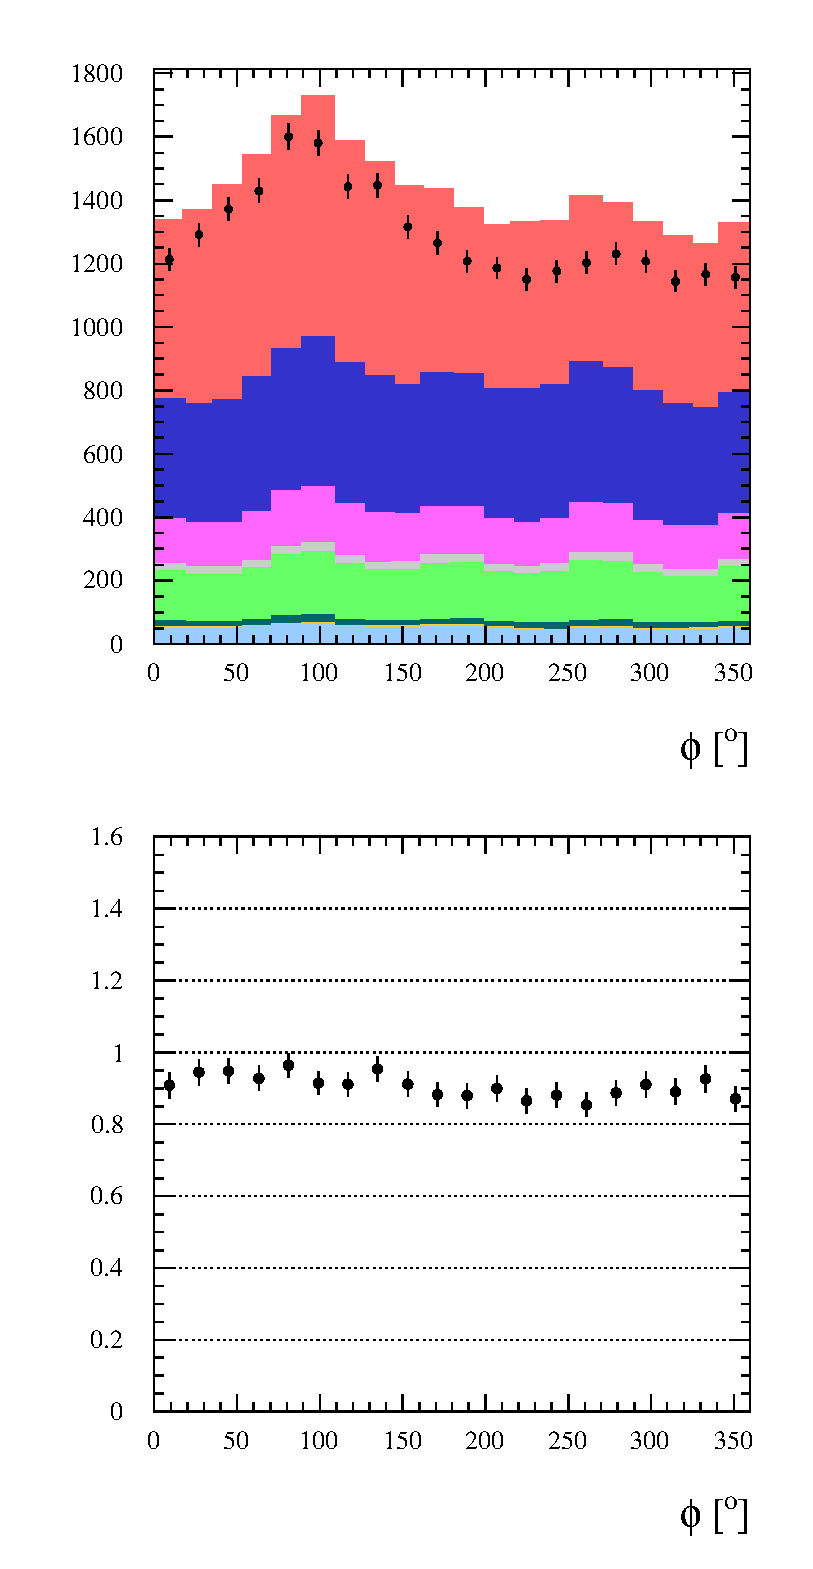
\includegraphics[width=3in]{Figures/P0DTrkPhiRun1Run2Run4.eps}
  \caption{Theta (left) and Phi (right) of the initial direction of 
the muon candidate track in Run 1, Run 2 and Run 4 'Water-in' periods. 
Below is the corresponding Data to MC ratio with statistical errors.} 
  \label{fig:ThetaRun1Run2Run4}%FIXME
\end{figure}

\begin{figure}
  \centering
  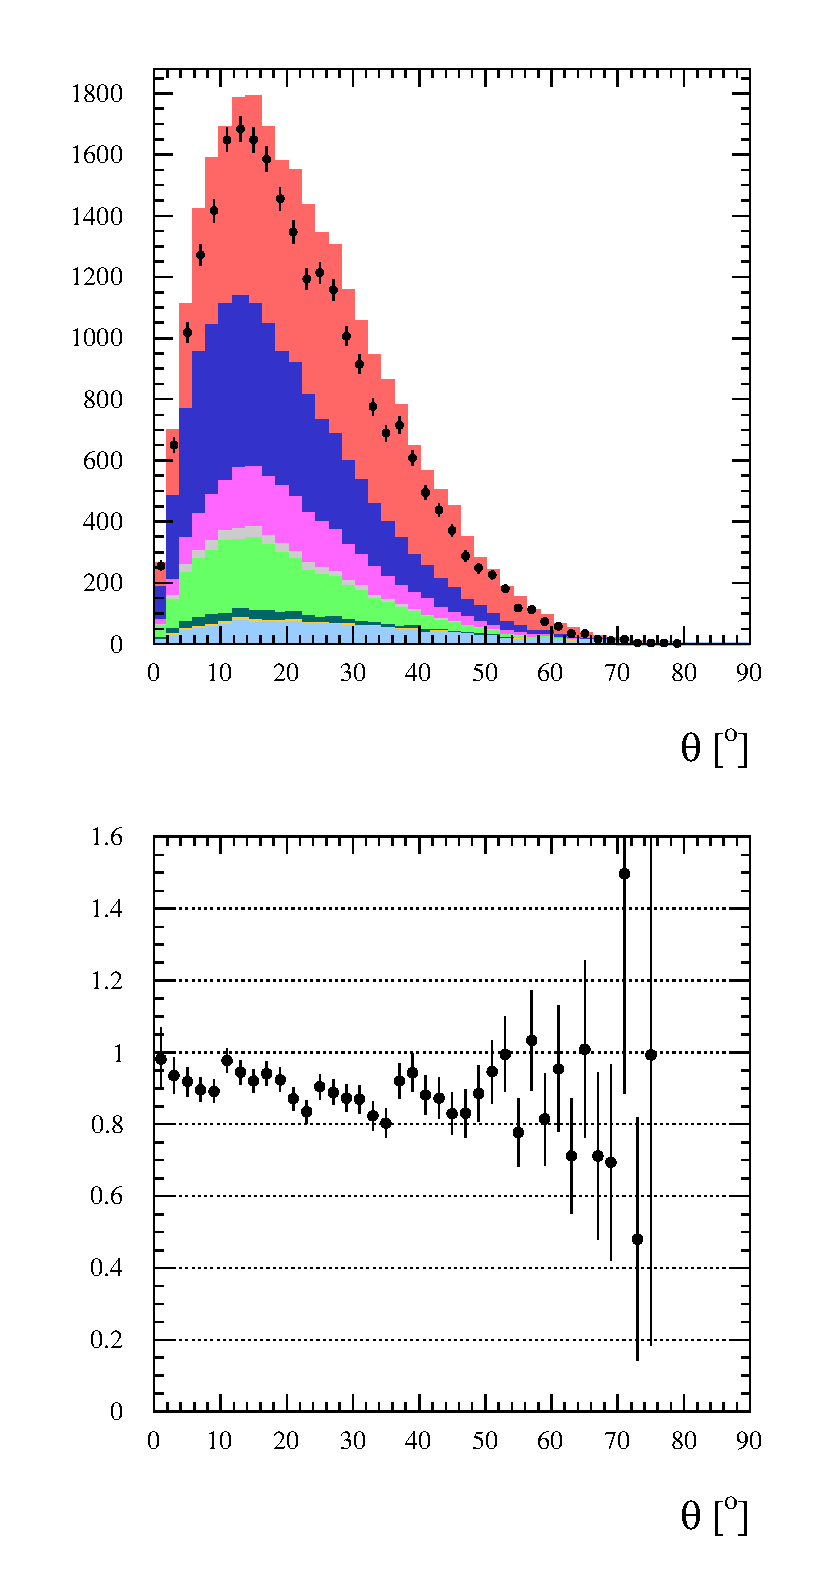
\includegraphics[width=3in]{Figures/P0DTrkThetaRun2airRun3airRun4air.eps}
  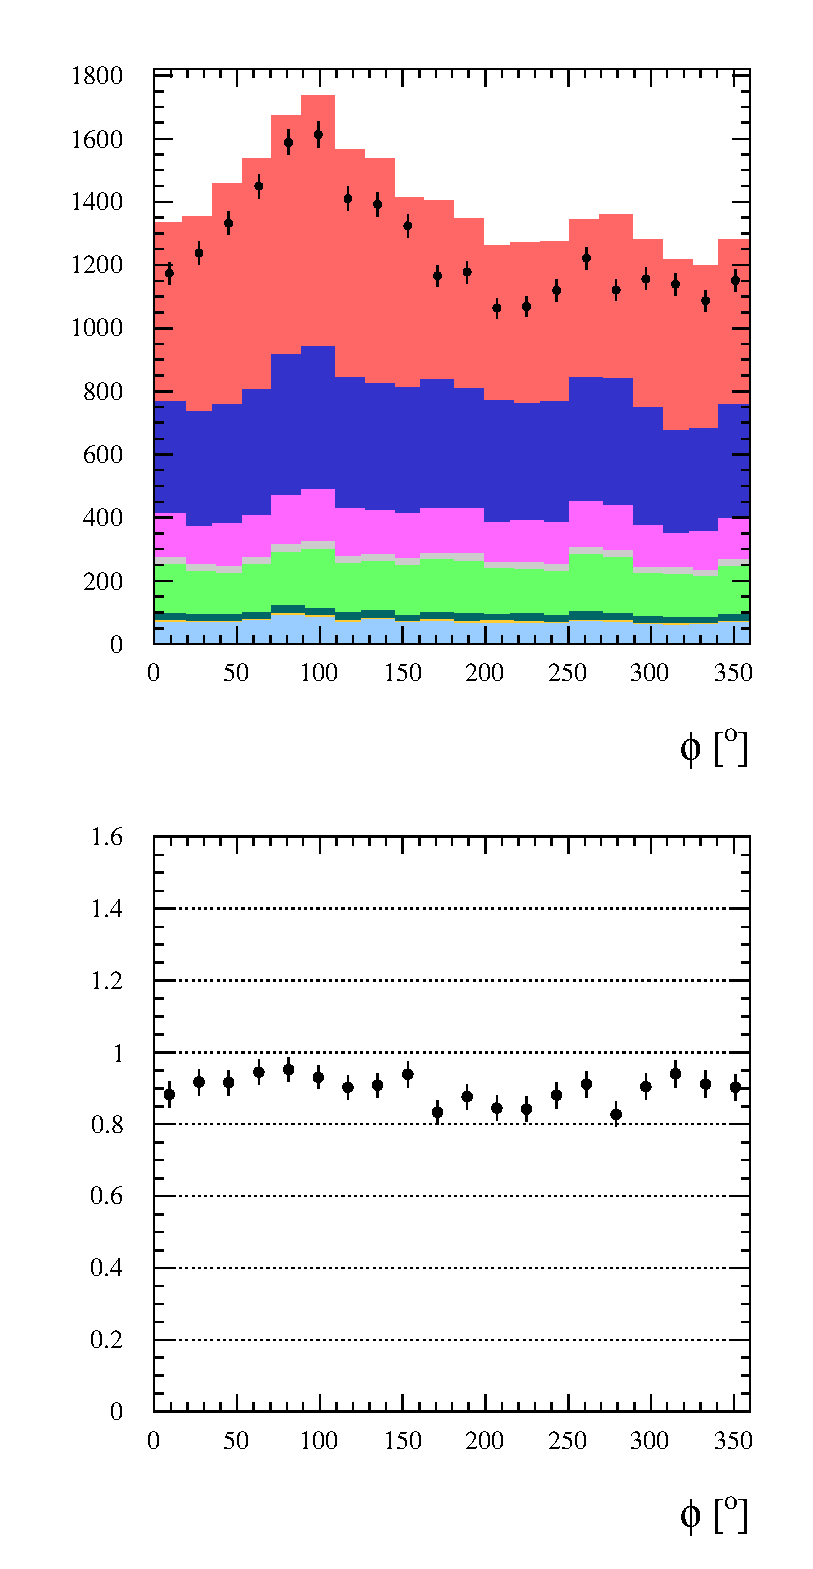
\includegraphics[width=3in]{Figures/P0DTrkPhiRun2airRun3airRun4air.eps}
  \caption{Theta (left) and Phi (right) of the initial direction of 
the muon candidate track in Run 2, Run 3 and Run 4 'Water-out' periods. 
Below is the corresponding Data to MC ratio with statistical errors.} 
  \label{fig:ThetaRun2airRun3airRun4air}%FIXME
\end{figure}

\subsubsection{Results}
\label{sec:RatioResults}

The result is reported as an integrated Data/MC ratio of the total 
selected CC inclusive interactions in Run 1, Run 2 and Run 4 
'Water-in' combined. 
The total events selected in Data is 
25,791 
which corresponds to 
an exposure of $23.6 \times 10^{19}$ POT. 
The unnormalized number of events selected in MC is 
1,031,295
for $626\times10^{19}$ POT. 
After normalizing MC by the Data POT 
and applying the fiducial mass correction (to each of the run periods 
as detailed in TN-073), 
we have yielded the Data/MC ratio of 
$ 0.879 \pm 0.006 $.\\

For completeness we summarized in Table \ref{tab:MCBreakdown} 
the number of events after all normalization and corrections 
for the different MC channels that we selected.

\begin{table}[h]
\centering
\begin{tabular}{lcc}
\toprule
MC Channel & & Number of events selected \\
\cline{1-1}\cline{3-3} 
QE & & 11,895 \\
Pi & & 8,294 \\
NPi & & 3,008 \\
Meason & & 480 \\
DIS & & 3,329 \\
NC & & 381 \\
$\bar{\nu}$ & & 98 \\
Other & & 7 \\
Out of FV & & 916 \\
\bottomrule
\end{tabular} 
\caption{
The number of events selected in the 
CC inclusive MC 
Run 1, Run 2 and Run 4 for the 'Water-in' periods 
combined sample, 
presented for the different MC channels. 
}
\label{tab:MCBreakdown} 
\end{table}

\begin{table}[h]
\centering
\begin{tabular}{lcc}
\toprule
MC Channel & & Number of events selected \\
\cline{1-1}\cline{3-3} 
QE & & 11,956 \\
Pi & & 7,700 \\
NPi & & 2,745 \\
Meason & & 440 \\
DIS & & 3,078 \\
NC & & 427 \\
$\bar{\nu}$ & & 110 \\
Other & & 7 \\
Out of FV & & 1,290 \\
\bottomrule
\end{tabular} 
\caption{
The number of events selected in the 
CC inclusive MC 
Run 2, Run 3 and Run 4 for the 'Water-out' periods 
combined sample, 
presented for the different MC channels. 
}
\label{tab:MCBreakdown} 
\end{table}

\clearpage

\clearpage
\clearpage
\section{Systematic Uncertainties in the Flux Prediction and Cross Section Model}
\label{sec:fluxxsecsyst}

There are three major sources of systematic uncertainty in our measurement:

\begin{itemize}
\item Flux prediction uncertainty
\item Cross section model simulation uncertainty
\item Detector level uncertainties caused by imperfect detector simulation
\end{itemize}

In this section, we describe the treatment of the first two sources of uncertainty, the flux prediction and the cross section model. Section \ref{sec:FluxDetermination} outlined the methodology behind extracting the uncertainty on the netrino flux at ND280. In Section \ref{sec:fluxsyst}, we complete the treatment of the flux uncertainty by propagating it through to our cross section measurement. Similarly, Section \ref{sec:evsim} discussed the parametrization and evaluation of the cross section model uncertainties and in Section \ref{sec:xsecsyst} we propagate these through to our measurement.

\subsection{Flux Prediction Systematic Uncertainty}
\label{sec:fluxsyst}

The flux systematic uncertainty is a large source of error in the cross section measurement. The majority of the uncertainty is due to the hadronic interaction model used with some small contribution from uncertainties in the proton beam alignment/angle and the horn current and field. As described in Section \ref{sec:FluxDetermination}, the flux uncertainty is parametrized by normalization factors in bins of neutrino or anti-neutrino energy. The $\nu_\mu$ flux is divided into 11 bins, the anti-$\nu_\mu$ into 5 bins, the $\nu_e$ into 7 bins and the anti-$\nu_e$ into 2 bins. The bin limits used are as follows (in GeV):

\begin{itemize}
\item $\nu_\mu$: 0, 0.4, 0.5, 0.6, 0.7, 1.0, 1.5, 2.5, 3.5, 5.0, 7.0, 30.0
\item anti-$\nu_\mu$: 0, 0.7, 1.0, 1.5, 2.5, 30.0
\item $\nu_e$: 0, 0.5, 0.7, 0.8, 1.5, 2.5, 4.0, 30.0
\item anti-$\nu_e$: 0, 2.5, 30.0
\end{itemize}

To propagate the flux error to our measurement, we use a 25 by 25 covariance matrix that encodes the current constraints on and correlations between the flux parameters. Figure \ref{fig:fluxcov} from Section \ref{sec:FluxDetermination} shows the flux covariance matrix used with bins for each of the neutrino types for ND280 and Super-K. The 25 bins at the bottom left of the flux covariance matrix shown are the ND280 flux bins that are used, the remainder are Super-K flux bins. We use a Cholesky decomposition technique \cite{chol} on the correlation matrix and multiply the resulting lower triangular matrix with a vector of 25 uncorrelated, gaussian, random values. The gaussians are centered at 1 and have a variance equal to the known variance of the corresponding flux bin. Each random vector multiplied by the decomposed correlation matrix yields a properly correlated ``throw'' of flux bin weights. When each flux bin weight is multiplied by the integrated flux in the given bin, each throw can be thought of as a new flux prediction. So for every new flux prediction, we have to recalculate the cross section value we aim to measure, and after many repeated throws, we produce a distribution of possible cross section measurements. The variance of this distribution tells us the uncertainty in our cross section measurement due to the uncertainty in the flux prediction at ND280. The Cholesky decomposition technique is a common mathematical tool and we use an implementation of the algorithm created by a T2K collaborator. The remainder of the flux uncertainty propagation is our work.

To recalculate the cross section for each flux throw, we re-evaluate six pieces of the cross section formula in \ref{eqn:xsec6}. We re-weight the MC and recalculate the background terms, efficiency terms and integrated flux terms. The same covariance matrix is used for all 4 beam runs. To reweight the integrated flux term, we first integrate the neutrino flux within the energy range of each $\nu_\mu$ flux bin. This integrated value is multiplied by the corresponding element, $w(i)$, of the thrown 25-element vector. This yields the new neutrino flux in that particular bin. We integrate over all 11 $\nu_\mu$ bins to calculate the new total flux as follows.

\begin{equation}
\Phi_{tot} = \sum_{i}^{11} \Phi^{new}(i) = \sum_{i}^{11} \left( w(i) \int^{bin\:hi\:edge}_{bin\:low\:edge} \Phi^{old}(i) dE_\nu \right).
\end{equation}

 The efficiency reweighting is done event by event. We use the energy of the neutrino that generated each event to find its corresponding $\nu_\mu$ flux bin. This in turn gives us the event weight for a particular flux vector throw. All the selected and unselected signal events are thus reweighted and the efficiency is recalculated. The background reweighting is done similarly. As our signal definition requires that the CC inclusive event be generated by $\nu_\mu$ only, the background term has some fraction of non-$\nu_\mu$ generated events. So while we only use the first 11 elements of the thrown flux weight vector for reweighting the integrated flux and signal efficiency terms, we use all 25 for the background reweighting. We calculate a weight for each background event using the interaction neutrino's type and energy to find the corresponding element in the thrown flux vector. Then the background terms are all recalculated. We take 5000 flux throws and therefore repeat the procedure 5000 times to create a smeared distribution of the cross section prediction due to flux uncertainties. This value was selected as a compromise between computing time required and the desire for highest possible statistics.

The results of 5000 variations of the flux uncertainties on the cross section is shown in Figure~\ref{fig:fluxvar}. We integrate the distribution from either extreme to find the cross section values that correspond to 15.9\% (area under normal distribution curve from -$\infty$ to -1$\sigma$) of all throws giving values below (or above for the upper limit) it. The integrated measurement has a fractional flux systematic uncertainty of -9.62\% and +11.09\%.

\begin{figure}[h]
\centering
\includegraphics[width=5in]{Figures/fluxvar.png}
\caption{A distribution of the calculated absolute water cross section for 5000 throws of the input flux. The input flux variations are calculated directly from throws of the ND280 bins of the flux covariance matrix.}
\label{fig:fluxvar}
\end{figure}

The cross section error on just the flux term is around $12\%$. However, we measure an overall error of less that $12\%$ on the cross section due to the subtraction method used. There is a larger fraction of out-of-fiducial background in the water-out selection than in the water selection. The background terms increase linearly with total integrated flux, whereas the efficiency terms remain roughly invariant as a function of flux. When calculating total expected signal events in water-in and water-out (N-B/eff.), the final value therefore varies inversely with the integrated flux term variation. However, the total expected signal in water-in data has a smaller variation that the signal in water-out due to smaller background fraction. So in effect, the total expected signal in water-only increases as integrated flux increases and decreases as integrated flux decreases. This correlation yields a smaller error due to flux uncertainty in this subtraction method.

\subsection{Cross Section Model Systematic Uncertainty}
\label{sec:xsecsyst}

The systematic uncertainty from the cross section model is another large contributor of error in this cross section measurement. To evaluate this error, we use reweighting software called T2KReWeight. This software was developed by several T2K working groups working together, and we were not directly involved with its development. This Section covers how we use T2KReWeight to propagate external physics model uncertainties to our absolute cross section measurement. Ideally, for every small variation in a cross section parameter, the MC would be regenerated. Then the particles would be repropagated and the events reconstructed and reselected. However, this is computationally intractable. Instead, the T2KReWeight software calculates the resulting MC variations on the fly by using precalculated response functions. 

For a variation in a physics parameter, the theoretical cross section in NEUT is recalculated. The ratio of the recalculated cross section and the nominal cross section is stored. This procedure is repeated for multiple variations in each physics parameter, storing the cross section ratios for each. This is handled by the reweighting capabilities of the neutrino generator being used, in this case NEUT. Afterwards, T2KReWeight takes a MC neutrino interaction, and based on the interaction type and other truth kinematics, uses the cross section ratios to calculate an event weight that is a ``reweighting" of the nominal event. This weight is directly related to the cross section ratio and is essentially a multiplicative factor describing the change in probability of the event occurring. As the MC truth information is available at all times, event weights can be generated at any given time, without needing to reprocess terabytes of data. Furthermore, while varying parameters like $M_A^{QE}$ requires help from NEUT, most of the cross section parameters are normalization factors. These factors are basically weights already as they can be directly applied to all events from a specific interaction mode (i.e. an increase in the CCQE normalization parameter of $10\%$ means an increase in the CCQE content of our samples by $10\%$ also). This reweighting method is used to quickly evaluate the effect of cross section model uncertainties on our measurement.

 The parametrization of the cross section model and the size of the corresponding errors were discussed in Section \ref{sec:evsim}. There are two types of cross section model uncertainties that were propagated. The first type are uncertainties in the 4-vector generation at the neutrino interaction vertex and the second type are the uncertainties in interactions that occur as a generated particle travels through the nucleus. The latter type of uncertainties are referred to as Final State Interaction (FSI) errors and are evaluated separately.

To estimate the neutrino interaction cross section model uncertainties, for each parameter, we generate an event weight for each selected Monte Carlo CC inclusive event and for each unselected true Monte Carlo CC inclusive event using T2KReWeight. The re-weighted Monte Carlo events will produce a new event cross section evaluated for a 1-sigma parameter excursion divided by the nominal parameter cross section. This is done for each parameter by evaluating weights at a $\pm$1-sigma excursion. Once each selected and unselected event has a weight, we re-evaluate the MC predicted backgrounds and efficiencies and finally the cross-section. The final error for each parameter leads to a fractional shift in the nominal cross section value

\begin{equation}
\delta(\sigma) = \frac{\sigma^{var.}-\sigma^{nom}}{\sigma^{nom}}.
\end{equation}

The positive and negative errors from each parameter variation are shown in Table \ref{tab:XSecPar}. The addition of these errors is not a straightforward task however, especially as the cross section parameters themselves are correlated. Ideally, we would take a throw from the correlation matrix in Figure \ref{fig:xseccorr} for the single pion fit parameters and use gaussian throws for the rest to perform the reweighting procedure multiple times. The resulting distribution of the water cross section values would then yield a total error from physics model uncertainty. This process is unfortunately too computationally intensive, so we use a simpler method. We note that the only two parameters from the single pion fit that affect the measurement appreciably are $M_A{RES}$ and CC 1$\pi$ normalization. The other single pion parameters are either not highly correlated or do not affect the water cross section. Looking closely at the $M_A^{RES}$ parameter, we find that if it increases (decreases), the cross section value decreases (increases). On the other hand, when the CC 1$\pi$ normalization increases (decreases), the cross section value also increases (decreases). Since $M_A^{RES}$ and the CC 1$\pi$ normalization are anti-correlated, upward excursions of $M_A^{RES}$ would suggest downward excursions of CC 1$\pi$ normalization. This is consistent with the cross section decreasing only. Similarly, a downward excursion of $M_A^{RES}$ would suggest an upward excursions of CC 1$\pi$ normalization, yielding an increase in the cross section. So conservatively, we linearly add the fractional cross section change from negative excursions of both parameters. The same is done for the positive excursions. From the values in the last two columns of Table \ref{tab:XSecPar}, this results in a combined $M_A^{RES}$ and CC 1$\pi$ normalization error of $+3.57\%$ and $-3.75\%$.

The rest of the parameters are assumed completely uncorrelated. Even though upward and downward excursions of each parameter cause the cross section to change in different directions, all the remaining errors are added in quadrature. Figures \ref{fig:xsvar1} and \ref{fig:xsvar2} shows the fractional change in the signal efficiency and background rate as a function of the Z vertex position binned by p0dule number. Only water-in MC is shown as the water-out results look very similar. Each plot has the $\pm 1 \sigma$ variation results for a single standard interaction cross section parameter. As the background rate and signal efficiencies are very small in certain regimes, the fractional change varies wildly in those areas, but have little impact on the final cross section measurement. The final systematic uncertainty due to the interaction physics model is $+8.78\%$ and $-13.43\%$. 

\begin{table}[h]
\centering
\caption{Cross section model parameter uncertainties and the resulting absolute water-only cross section fractional error.}
\begin{tabular}{lcccc}\toprule\midrule
\renewcommand{\arraystretch}{1.1}
Parameter &  Value & Error & + Var. (\%) & - Var. (\%)
\\ \midrule
M$_A^{QE}$ & 1.21GeV$^2$ & 0.45 GeV$^2$ & 3.9 & -7.33\\
\midrule
M$_A^{RES}$ & 1.16GeV$^2$ & 0.11 GeV$^2$ & 0.86 & -0.89\\
\midrule
Spectral Function & off & on/off & 0 & -4.01\\
\midrule
Fermi Momentum & 217 MeV/c  & 30 MeV/c & 0.81 & -0.77\\
\midrule
Pionless Delta Decay & 0.2 & 0.2 & 0.21 & -1.05\\
\midrule
DIS/Multi-Pi Shape & 1.0 & 0.4 &  0.46 & -0.44\\
\midrule
CC QE Norm. (E$_\nu < 1.5$~GeV) & 1.0 & $0.11$ & 2.81 & -2.90\\
\midrule
CC QE Norm. (3.5~GeV$>$ E$_\nu > 1.5$~GeV) & 1.0 & $0.30$ & 1.83 & -1.73\\
\midrule
CC QE Norm. (E$_\nu > 3.5$~GeV) & 1.0 & $0.3$ & 1.75 & -1.66\\
\midrule
CC Res Norm. (E$_\nu < 2.5$~GeV) & 1.63 & $0.43$ & 2.71 & -2.85\\
\midrule
CC Res Norm. (E$_\nu > 2.5$~GeV) & 1.0 & $0.4$ & 5.65 & -4.80\\
\midrule
CC Coh Norm. & 1.0 & $1.0$ & 1.42 & -1.31\\
\midrule
%NC COh Norm. & 1.0 & $0.3$ & 0.01 & -0.01\\
%\midrule
%NC 1Pi Norm. & 1.0 & $0.3$ & 0.01 & -0.01\\
%\midrule
NC Other Norm. & 1.0 & $0.3$ & 0.24 & -0.24\\
\midrule
MiniBoone CC 1Pi E$_\nu$ Shape. & off & on/off & 0.0 & -7.45\\
\midrule
\midrule
Total Interaction Systematic & &&$+8.78\% $  & $-13.43\%$  \\
\midrule
\bottomrule
\end{tabular}
\label{tab:XSecPar}
\end{table}

\newpage
\clearpage
\begin{figure}[h]
\centering
\includegraphics[width=5in]{Figures/TN100Plots/c_6_0.png}
\caption{The fractional change in the water-in signal efficiency (predicted from MC) as a function of p0dule number of neutrino interaction vertex for a +1 $\sigma$ (blue) and -1$\sigma$ (red) variation of cross section parameter. From left to right, top to bottom, the cross section parameters varied are: MAQE, MARES, DIS Multi-Pi Shape, Spectral Function, Fermi Momentum, Pion-less Delta Decay, CCQE Norm. ($E_\nu < 1.5$GeV), CCQE Norm. ( 3.5~GeV$E_\nu>1.5$GeV), CCQE Norm ($E_\nu > 3.5$GeV), CC 1Pi Norm. ($E_\nu < 2.5$GeV), CC 1Pi Norm. ($E_\nu > 2.5$GeV), CC Coh Norm., NC Coh Norm., NC 1Pi Norm., NC Other Norm., MiniBoone CC 1Pi $E_\nu$ Shape.}
\label{fig:xsvar1}
\end{figure}

\newpage
\begin{figure}[h]
\centering
\includegraphics[width=5in]{Figures/TN100Plots/c_12_0.png}
\caption{The fractional change in the water-in background (predicted from MC) as a function of p0dule number of neutrino interaction vertex for a +1$\sigma$ (blue) and -1$\sigma$ (red) variation of cross section parameter. From left to right, top to bottom, the cross section parameters varied are: MAQE, MARES, DIS Multi-Pi Shape, Spectral Function, Fermi Momentum, Pion-less Delta Decay, CCQE Norm. ($E_\nu < 1.5$GeV), CCQE Norm. ( 3.5~GeV$E_\nu>1.5$GeV), CCQE Norm ($E_\nu > 3.5$GeV), CC 1Pi Norm. ($E_\nu < 2.5$GeV), CC 1Pi Norm. ($E_\nu > 2.5$GeV), CC Coh Norm., NC Coh Norm., NC 1Pi Norm., NC Other Norm., MiniBoone CC 1Pi $E_\nu$ Shape.}
\label{fig:xsvar2}
\end{figure}

The FSI error is evaluated following the procedure in Section \ref{sec:evsim}. There are 16 combinations of variations used for the FSI parameters to fully account for the necessary uncertainty. Each combination of 16 parameter variations is fed through T2KReWeight and the water cross section is recalculated. The fractional change from the nominal cross section is given as the error as before. The water cross section error from each combination are averaged together to yield the FSI uncertainty contribution. The results are shown in Table \ref{tab:XSecFSI}.

\begin{equation}
\sigma_{avg}^2 = \sum_i^{16} \frac{\sigma_i^2}{16}
\end{equation}

\begin{table}[h]
\caption{Final State Interaction parameter uncertainties and the resulting water-only cross section fractional error.}
\centering
\begin{tabular}{cccccccc}\toprule\midrule
\renewcommand{\arraystretch}{1.1}
Comb.& Inel Lo & Inel Hi & Pi Prod. & Pi Abs. & Ch Ex Lo & Ch Ex Hi & Error
\\ \midrule
1 & 0.6 & 1.1 & 1.5 & 0.7 & 0.5 & 2.3 & 0.23\%\\
\midrule
2 & 0.6 & 1.1 & 1.5 & 0.7 & 1.6 & 2.3 & 0.56\%\\
\midrule
3 & 0.7 & 1.1 & 1.5 & 1.6 & 0.4 & 2.3 & 0.16\%\\
\midrule
4 & 0.7 & 1.1 & 1.5 & 1.6 & 1.6 & 2.3 & 0.27\%\\
\midrule
5 & 1.4 & 1.1 & 1.5 & 0.6 & 0.6 & 2.3 & 0.45\%\\
\midrule
6 & 1.3 & 1.1 & 1.5 & 0.7 & 1.6 & 2.3 & 0.33\%\\
\midrule
7 & 1.5 & 1.1 & 1.5 & 1.5 & 0.4 & 2.3 & -0.44\%\\
\midrule
8 & 1.6 & 1.1 & 1.5 & 1.6 & 1.6 & 2.3 & -0.03\%\\
\midrule
9 & 0.6 & 2.3 & 0.5 & 0.7 & 0.5 & 1.3 & 0.46\%\\
\midrule
10 & 0.6 & 2.3 & 0.5 & 0.7 & 1.6 & 1.3 & 0.34\%\\
\midrule
11 & 0.7 & 2.3 & 0.5 & 1.6 & 0.4 & 1.3 & 0.30\%\\
\midrule
12 & 0.7 & 2.3 & 0.5 & 1.6 & 1.6 & 1.3 & 0.30\%\\
\midrule
13 & 1.4 & 2.3 & 0.5 & 0.6 & 0.6 & 1.3 & 0.30\%\\
\midrule
14 & 1.3 & 2.3 & 0.5 & 0.7 & 1.6 & 1.3 & -0.01\%\\
\midrule
15 & 1.5 & 2.3 & 0.5 & 1.5 & 0.4 & 1.3 & -0.37\%\\
\midrule
16 & 1.6 & 2.3 & 0.5 & 1.6 & 1.6 & 1.3 & -0.31\%\\
\midrule
Total & & & & & & & 0.34\%\\
\midrule
\bottomrule
\end{tabular}
\label{tab:XSecFSI}
\end{table}

The total error in the absolute water cross section measurement is +8.79\% and -13.43\% when FSI and standard interaction uncertainties are added in quadrature. We note that there is some model dependence in our measurement that is introduced through the MC estimate of the background interactions. Also, a majority of the background contamination is OOFV CC inclusive events. As this background still consists of CC inclusive events (albeit outside the fiducial volume) we are using the MC to model not only the contamination rate of the OOFV events, but also the rate of CC inclusive events. This implies that there is some signal model dependence in our measurement. As the variation of $M_A^{QE}$, a parameter that controls a signal interaction mode, caused a 7\% shift in the cross section measurement, the model dependence is not negligible.

\newpage
\subsection{P0D Tracking and Matching Efficiency}
\label{sec:Systematics_Efficiency}

The efficiency of reconstruction, and the differences between Monte Carlo and data efficiencies, are the first source of systematic uncertainty studied for the CC Inclusive selection. There are several steps involved in reconstructing the final candidate muon track as described in previous sections. In this section, we use a `FGD Cosmic' sample to  investigate the reconstruction and matching efficiencies of our analysis. Cosmics provide a sample independent of the physics we are probing, and are an excellent unbiased sample to use to evaluate the efficiency systematic. However, as Cosmics do not have the same bunched timing structure as our beam events, we also used as independent sample of sand muons from Production 4 to cross check our results. The results of the cross check are summarized in Section \ref{sec:Appendix_sandmuoneff}. Efficiencies extracted from Production 4 cosmics and sand muons and Production 5 cosmics agree well.
Sand Muons are generated by beam neutrinos interacting with material outside the off-axis near detector and so have a timing strucutre that mimics that of beam events. 
These two 'sideband' samples together provide a robust method for evaluating the matching and reconstruction efficiency systematic. Finally, we also performed a hand-scan of beam events in Production 4 reconstruction files to identify and quantify any reconstruction issues missed with the FGD cosmics and sand muon samples.\\

We use a simple method to examine the efficiency of our matching algorithm for tracks that deposit energy in the \p0d, enter the Tracker and are reconstructed by the Tracker reconstruction package. We simultaneously determine how often P0D reconstruction successfully fits a track and how often we succesfully match this track with a Tracker reconstructed track. First, we pre-select a sample of quality tracks reconstructed in TPC1 that point squarely into the 
\p0d. We then attempt to pair each of these tracks to a \p0d reconstructed track. The ratio of the number of matched pairs found to the number of quality TPC1 tracks yields the 'matching efficiency'. Though this estimate is not necessarily the absolute efficiency, given that monte carlo simulates data well to the first order, the observed difference between the monte carlo efficiency and the data efficiency gives us the systematic due to reconstruction and matching.

This definition folds in the \p0d's intrinsic, lower level reconstruction efficiencies (i.e. hit finding, \p0d-only tracking, etc.) as well as matching and recombination efficiencies from the matching algorithm. However, as we use reconstructed tracks in the ND280 Tracker as a baseline, we do not account for the Tracker tracking efficiency with this strategy. We determine the systematic uncertainty from the Tracker efficiency separately in a later section.\\

\subsubsection{Cosmics Sample}
\label{sec:CosmicsEfficiency}

Using the `FGD Cosmics' sample, we extract the matching efficiency as defined above. The following determine the denominator and numerator. Note that for the numerator of the efficiency, the cuts closely mimic those used in Sections \ref{sec:EventReconstruction} and \ref{sec:InclusiveAnalysis} to select muon candidates. Also, the pre-selection cuts are slightly different between the Cosmics sample as opposed to the Sand Muon sample. The necessity for this difference is discussed later.\\

Pre-Selection Cuts (Denominator):

\begin{enumerate}
\item There must be a Tracker reconstructed track in the event
\item The Tracker track must be reconstructed as beginning at the upstream face of the first TPC (Z \(<\) -750 mm)
\item The TPC must measure a momentum of at least 250 MeV
\item Project the Tracker track linearly backwards into the \p0d. The projection is made to the Z = -1100 mm plane, and then just the XY fiducial cut is applied to the projected point.
\item The Tracker track has \(>\) 18 reconstruction nodes
\item The Tracker track has a `corrected time' stamp between -4800ns and -4400ns. The time correction allows us to find the tracker time in relation to the \p0d electronics. The time cut is placed 80ns from the edge of the 480ns-wide \p0d integration window. This is the window where the \p0d electronics are capable of properly reconstructing hits. For a more detailed discussion of the timing cut, please refer to Appendix section \ref{sec:Appendix_p0delec.}
%\item There are at least 3 `good \p0d hits'. A `good hit' is defined as a 7 p.e. or greater \p0d hit which is found within a certain region of the \p0d and with a certain time. The region we search is a cone with opening angle of 30 degrees and length of 250mm. The time is required to be 80ns from the edge of the \p0d integration window. We make this cut to assure that no noise hits or hits with invalid timing due to known electronics design, are contaminating our pre-selection. For a more detailed discussion of the timing cut, please refer to Appendix section \ref{sec:Appendix_p0delec.}
\end{enumerate}

Matching Cuts (Numerator):
\begin{enumerate}
\item All pre-selection cuts are made as above
\item P0D Vertex must be reconstructed by TP0DPairwiseVertexPID algorithm and the track must be a constituent of this vertex
\item P0D Track must be exiting as defined by the last node having a Z position $>$ -1016 mm
\item P0D Track must be 3D as defined by cutting on track position variance
%\item Correct for alignment (x = 7 mm, y = 26 mm) in data only. 
Evaluate $\Delta R$, $\Delta \sin \theta$  and $\Delta T$ between the p0d track projection and tracker track as before. Apply the following cuts: $\Delta R$ \(<\) 86mm, $\Delta \sin \theta$ \(<\) .76, $\Delta T$ \(<\) 100 ns.
\end{enumerate}

The number of tracks passing the numerator cuts divided by the number passing the denominator cuts yields the efficiency. Figures \ref{fig:eff_dR} and \ref{fig:eff_dSdT} show the matching parameter distributions for $\Delta R$, $\Delta X$, $\Delta Y$, $\sin \Delta \theta$ and $\Delta T$. 
The $\Delta Y$ distribution does not agree very well and causes some disagreement in the $\Delta R$ distribution as well. This discrepancy has been isolated to a difference between forward going and backwards going cosmics tracks as determined by the Tracker reconstruction. Figure \ref{fig:dY} shows the $\Delta Y$ residuals separated by forward and backwards going tracks for FGD Cosmics in Data and MC. Note that in MC, the two different directions have a small shift in the central value of the residual. However, in Data, the shift is much greater. Using Production 4 to demonstrate the effect, we have fit gaussians to all of the residuals. The results are shown in Table \ref{tab:FitdY}. The root cause of this effect is a difference in the geometry used for reconstruction and the geometry of the `as built' detector. A much more detailed investigation and the results are discussed in the Appendix in Section \ref{sec:Appendix_align}. Finally, note that since the $\Delta R$ agreement between Data and MC for the Cosmics sample is actually worse than the Beam events, the evaluated uncertainty should be conservative. 
Similarly, though the timing distribution does not agree as well as the others, the timing cut is large enough to account for the overall shift. 


\begin{figure}
\centering
\includegraphics[width=2.5in]{Figures/Systematics/MatchingEfficiency/datadY.eps}
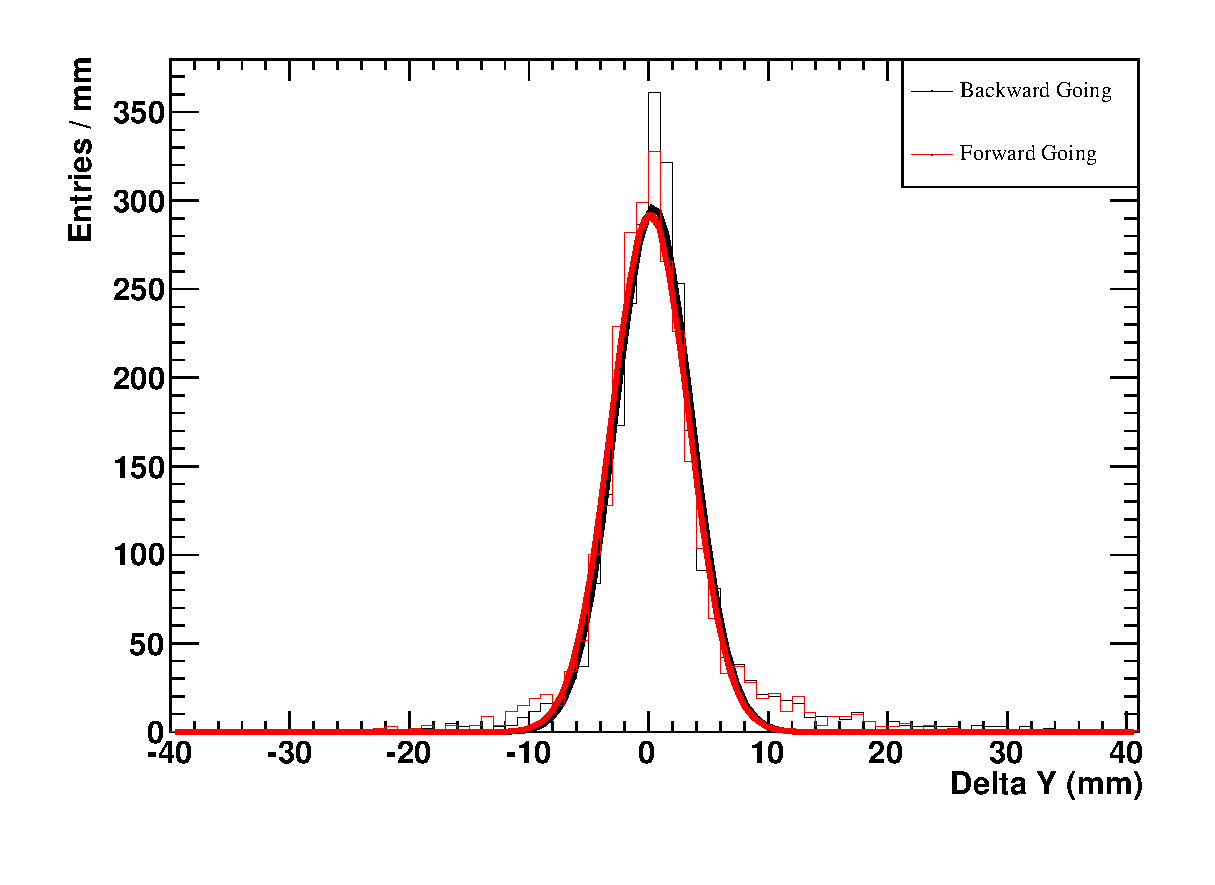
\includegraphics[width=2.5in]{Figures/Systematics/MatchingEfficiency/mcdY.eps}
\caption{
Matching Parameter $\Delta$ Y for Production 4 FGD cosmics in Data and MC split into forward and backward going tracks. Gaussian fits have been overlayed. The left plot shows the shift in the residual in Data cosmics when comparing forward (red) and backward (black) tracks. The right plot shows that in MC we do not see such a shift between forward (red) and backward (black) tracks.
}
\label{fig:dY}
\end{figure}

\begin{table}
\centering
\begin{tabular}{lccc}\toprule\midrule
Type and Dir. &  Mean & Sigma & $\chi^2$/NDOF \\ \midrule
Data Forward & $-4.1\pm 0.1$ & $4.1\pm 0.1$ & $100.0/48$  \\
\midrule
Data Backward & $3.1\pm 0.1$ & $4.5\pm 0.1$ & $155.2/58$ \\
\midrule
MC Forward & $0.1\pm 0.1$ & $3.2\pm 0.1$ & $255.1/51$ \\
\midrule
MC Backward & $0.5\pm 0.1$ & $3.2\pm 0.1$ & $263.2/59$ \\
\bottomrule
\end{tabular}
\caption{Gaussian fit results and fit error of $\Delta Y$ for 10000 Production 4 FGD Cosmics in Data and MC. The results are divided into backwards and forward going cosmics as determined by the Tracker reconstruction.}
\label{tab:FitdY}
\end{table}

\begin{figure}
\centering
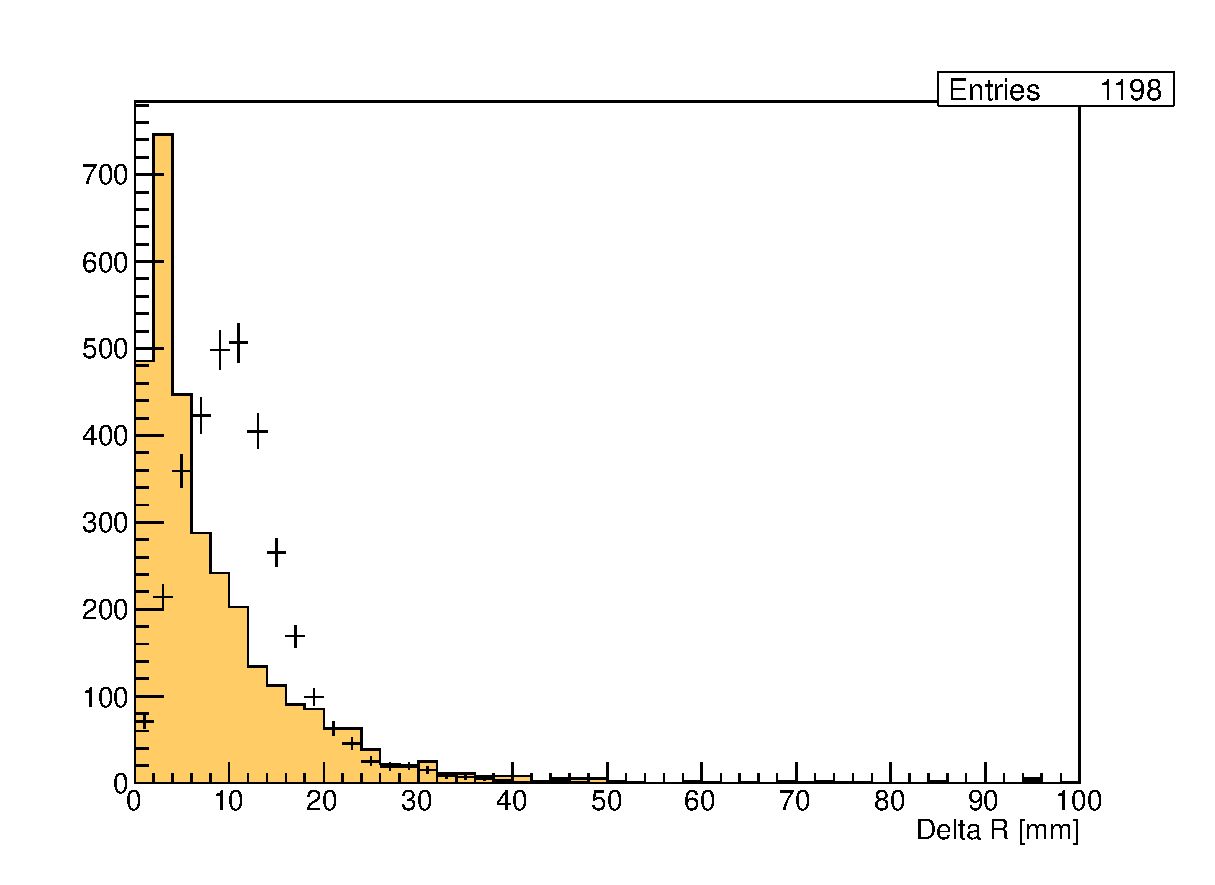
\includegraphics[width=2in]{Figures/Systematics/MatchingEfficiency/dRcosmics.eps}
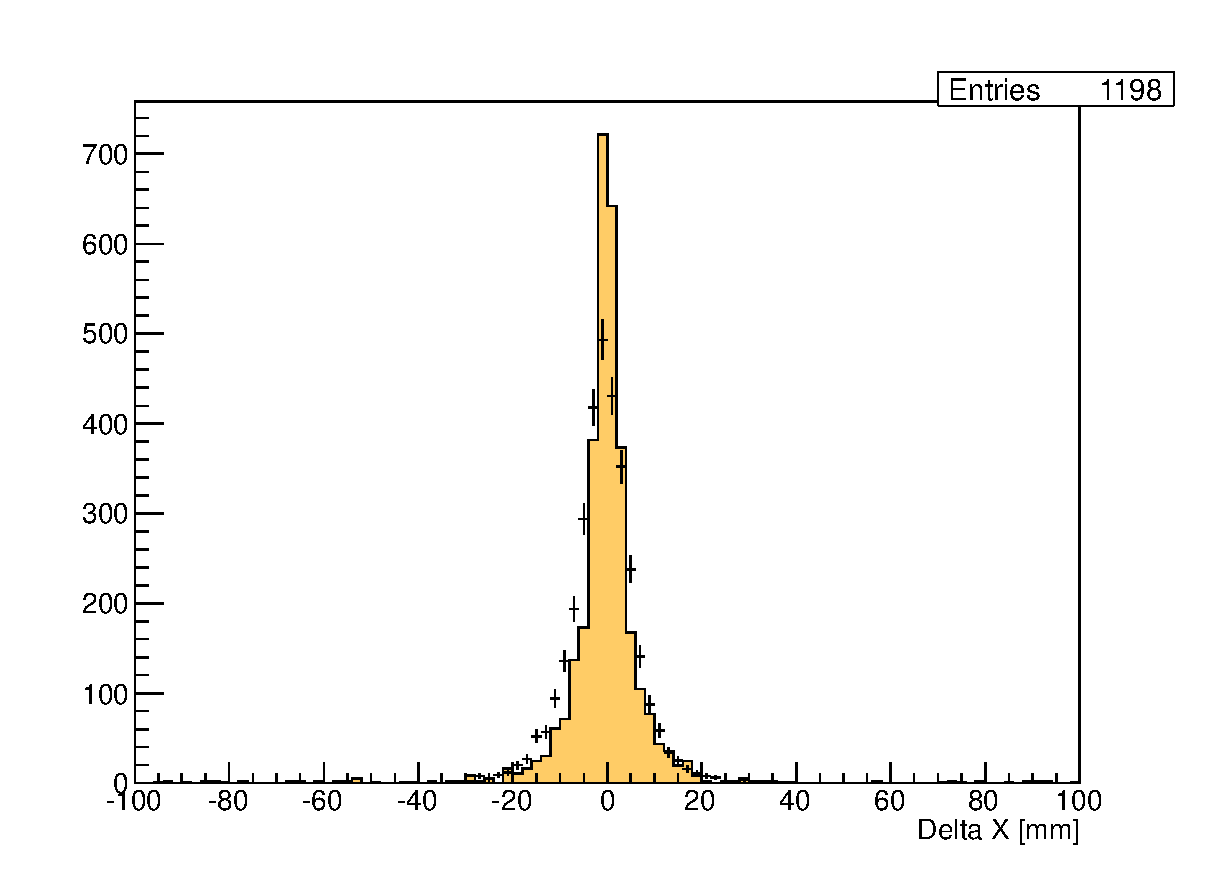
\includegraphics[width=2in]{Figures/Systematics/MatchingEfficiency/dXcosmics.eps}
\includegraphics[width=2in]{Figures/Systematics/MatchingEfficiency/dYcosmics.eps} 
\caption{
Matching Parameters $\Delta$ R, $\Delta$ X, and $\Delta$ Y for cosmics. The matching cut is applied only on $\Delta$ R. Black dots with error bars denote data while the orange fill is monte carlo. We note that the difference in shape in $\Delta$ R distributions is due to a shape difference in $\Delta$ Y between data and MC.
}
\label{fig:eff_dR}
\end{figure}

\begin{figure}
\centering
\includegraphics[width=2.5in]{Figures/Systematics/MatchingEfficiency/dScosmics.eps}
\includegraphics[width=2.5in]{Figures/Systematics/MatchingEfficiency/dTcosmics.eps}
\caption{Cosmics matching efficiency parameters \(\sin \theta\) and \(\Delta T\). The difference in \(\Delta T\) is not understood, but the cut is placed wide enough to be insensitive to the overall shift.}
\label{fig:eff_dSdT}
\end{figure}

\begin{figure}
\centering
\includegraphics[width=3in]{Figures/Systematics/MatchingEfficiency/Eff_vs_Momentum.eps}
\includegraphics[width=3in]{Figures/Systematics/MatchingEfficiency/Eff_vs_Theta.eps}
\caption{Cosmics efficiencies as a function of Momentum and \(\theta\). Black dots are data and red line is the MC. The orange fill shows the error on the MC. We note that the data and MC efficiencies track each other as a function of both kinematic variables.}
\label{fig:eff_ND}
\end{figure}

Figure \ref{fig:eff_ND} then shows the final efficiency values for data and MC as a function of muon momentum and $\theta$. Note that in Figure \ref{fig:eff_ND}, the statistical errors are calculated using a probability distribution function derived with a bayesian approach. The derivation of the PDF can be found in a paper by M. Paterno~\cite{bayes} and is implemented in ROOT under the TEfficiency class. The central values in Figure \ref{fig:eff_ND} are then the mean of the PDF (as opposed to the median). The statistical error for the integrated ratio is calculated more simply by approximating the efficiency as a binomial distribution. The efficiencies from the FGD cosmics sample are $99.08\%\pm 0.16\%$ for Data and $99.22\%\pm 0.24\%$ for MC.

\subsubsection{Reconstruction Failures in Beam Events}

We also performed a search for unclassified reconstruction failures in beam events in Production 4 to account for any possible systematic effect missed by the FGD cosmics and sand muons study. Similar to the method in Section \ref{sec:CosmicsEfficiency}, beam events with one or two quality Tracker tracks pointing directly into the P0D were pre-selected. As the Data has a large number of sand muons present, we also added a cut to veto these events. If more than two above-noise hits were found in the outer edges of the \p0d coincident in time with the TPC1 track, we tag the event as a sand muon and exclude it. Of the remaining events, we filtered out those where the matching algorithm failed to find a suitable \p0d track to match with the Tracker piece. Finally, the filtered events were examined by hand using an event plotting software (plot-event.exe) to identify any potential reconstruction pathologies previously missed.

When hand scanning filtered events, we founds several modes of failure, many of which were expected. For example, events which had short or partially reconstructed tracks in the downstream end of the \p0d as well events with no \p0d constituent were missed by the matching algorithm for obvious reasons. Furthermore, some DIS-like events had large clusters of energy deposits in the \p0d and were difficult to separate properly into tracks. These were also missed by the matching algorithm as expected. However, there were three classes of failure which, by eye, looked as if they should have been successfully matched. These we examined more closely.

First, we found events with multiple clean tracks passing into TPC1 which were missed by our algorithm. Further study showed this failure mode existed both in Data and MC and was an expected effect. In Appendix Section \ref{sec:Appendix_ambig} we explain how a reconstruction amibiguity (due to design) causes a small portion of multi track events to fail the matching algorithm. Second, we found another class of failed events where the \p0d and Tracker tracks were well matched spatially, but separated widely in time ($\Delta T$ failure). Finally, the last failure mode were events where the \p0d and Tracker tracks were mismatched in the XZ projection, a symptom of incorrect T0 extraction at the TPC1 reconstruction stage. An incorrect T0 calculation creates an offset in the TPC drift direction (XZ). Please see the ND280 reconstruction technical note \cite{tn72} for greater detail. Figure \ref{fig:mismatchexamples} shows examples of the $\Delta T$ and $T0$ failure modes.

\begin{figure}[h]
  \centering
  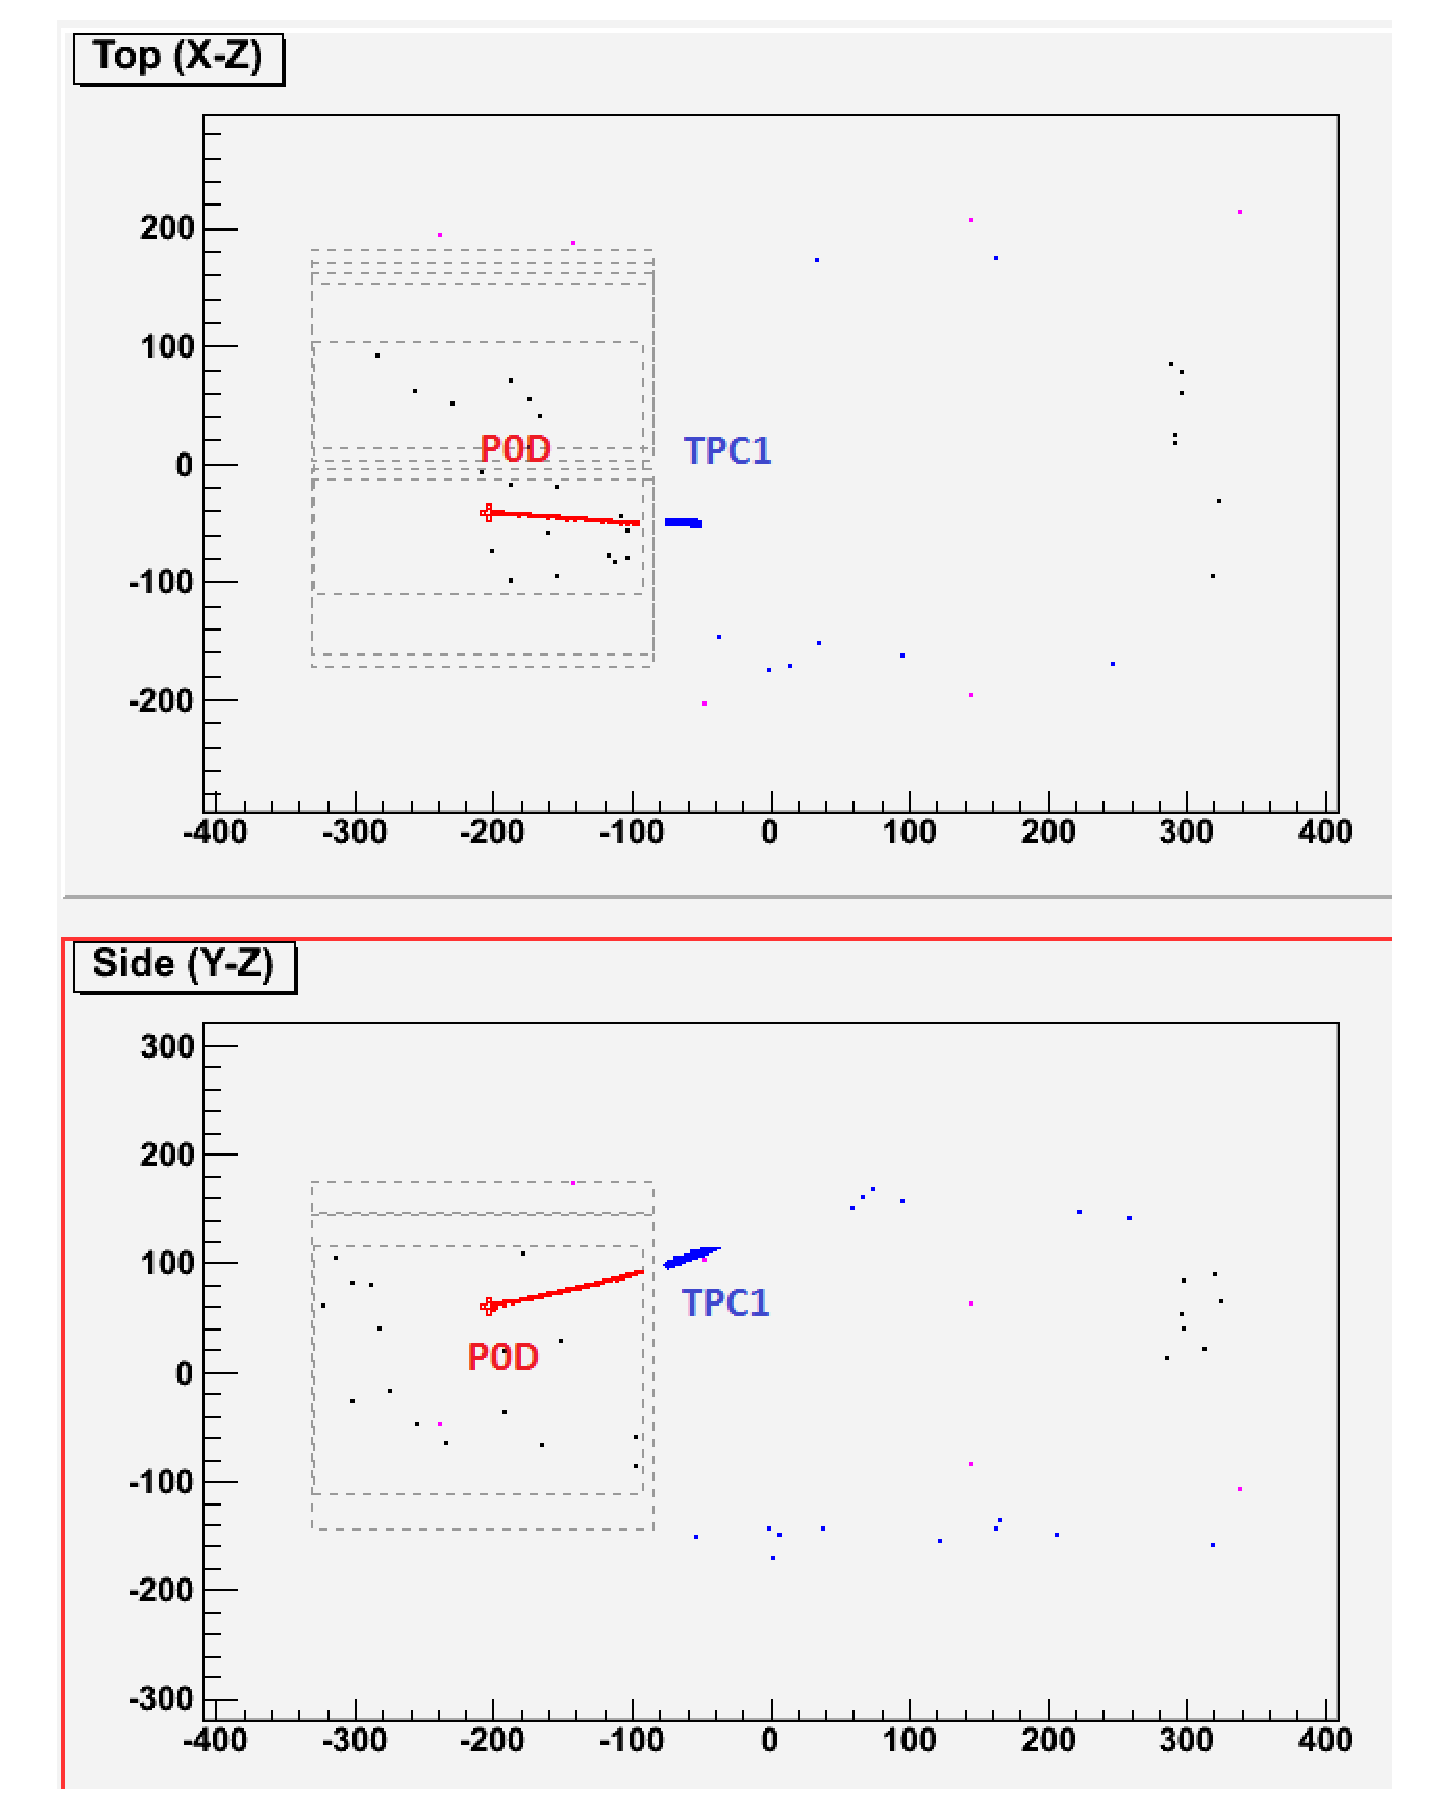
\includegraphics[width=3in]{Figures/delltaTmismatch.eps}
  \includegraphics[width=3in]{Figures/t0mismatch.eps}
  \caption{An example of the $\Delta T$ (left) and $T0$ (right) failure modes. In the  $\Delta T$ failure, the \p0d track (red) and the Tracker track (blue) match perfectly spatially, but are disjoint in time by $>100$ns. In the $T0$, the YZ projection has a good spatial match between the \p0d track (red) and Tracker track (yellow), but the drift direction shows a symptomatic offset.} 
  \label{fig:mismatchexamples}
\end{figure}

We hand scanned Data events corresponding to $1.056\times 10^{19}$POT and MC events corresponding to $3.34\times 10^{18}$POT. The two timing related failure modes, $T0$ and $\Delta T$, were only observed in Data and never in MC. Closer examination of the failed events showed that though some were muon-like tracks originating inside the \p0d, many were actually sand muon events which made it through the veto. As the timing of the TPC1 track piece and the \p0d track piece were generally different in these events, our sand muon veto did not associate the hits in the outer edges of the \p0d with the TPC1 track, causing the sand muons to leak through our selection cuts. In Table \ref{tab:handscan} we summarize the number of events in Data that failed via the $T0$ and $\Delta T$ modes and whether they originated from inside or outside the \p0d.
\begin{table}[here]
\centering
\begin{tabular}{lcc}\toprule
& $\Delta T$ Failures & $T0$ Failures\\\midrule
Sand Muon & 11 & 20 \\
In-\p0d Muon & 10 & 9 \\\bottomrule
\end{tabular}
\caption{
Total number of events from the $\Delta T$ and $T0$ failure modes for sand muons and in-\p0d muon-like events.
}
\label{tab:handscan}
\end{table}

An examination of the $\Delta T$ failures show that none of the tracks have FGD constitutents. As the two control samples are predominantly tracks that pass through the FGD, the $\Delta T$ failure is most likely not accounted for in the efficiencies evaluated using Sand Muons and FGD Cosmics. We use the 10 $\Delta T$ In-\p0d failures as uncertainty in the Data event rate. 
Sand muon events which made it past our veto in this study would still be correctly rejected in the actual CC inclusive selection by the fiducial volume cut. However, the T0 effect is not necessarily replicated correctly in the cosmics and sand muon samples. When relatively steep tracks pass through TPC1 without also entering an FGD, the T0 is more likely to be miscalculated. Since FGD cosmics require the tracks to pass through the FGDs and sand muons are generally lengthy tracks passing through the entire ND280, T0 problems are less likely observed. So the hand scan study also adds a matching uncertainty due to the 9 muon-like tracks corresponding to the T0 failure mode. Also, even though the study was conducted on Production 4, we expect the errors to persist in Production 5 as the effect stems from tracks lacking FGD constituents.

Including the statistical errors appropriately, we have $19\pm 4.36$(stat.) events more in the Data from the T0 failure and the In-\p0d $\Delta T$ failure modes combined. When normalized to the total Data POT for each run type from the inclusive analysis, we get $422.28 \pm 96.88$  events per $23.47\times 10^{19}$POT for water-in running and $591.77 \pm 135.76$  events per $32.89\times 10^{19}$POT for water-out running.

\subsubsection{Results of Matching Efficiency Systematic Studies}
\label{sec:Systematics_MatchingEfficiencyResults}

From the FGD cosmic sample, the MC / Data efficiency ratio is $(99.22\%\pm 0.24\%) / (99.08\%\pm 0.16\%) = 100.14\%\pm 0.24\%$. This is the value we need to multiply the final Data to MC ratio by to correct for efficiency. Similarly, using the results from the hand-scanning procedure, we calculate corresponding correction factors of $1.017 \pm 0.0039$ for water-in and $1.023 \pm 0.0053$ for water-out. These correction factors are multiplicative and uncorrelated with the cosmics efficiency correction. Propagating errors in quadrature yields total correction factors of $1.018 \pm 0.0049$ for water-in and $1.024 \pm 0.0060$ for water-out. The Data to MC ratios are shifted by using this final correction factor. The corresponding errors are then $\pm 0.49 \%$ for water-in runs and $0.6 \%$ for water-out runs.

%Linearly adding and subtracting the error and the central value, we get the efficiency ratio ranges of 99.18\% to 99.92\% from cosmics and 99.83\% to 100.36\% from sand muons. Taking the widest possible limits, we get the range 99.18\% to 100.36\%. To this range, we add the results from the hand scanning study. Missing events in Data only adds to the efficiency systematic number. 
%So taking the lower and upper limits of the hand scanning result, we get a $(62-21) / 7845 = 0.0052$ shift in the lower limit of the efficiency systematic and a $(62+99) / 7845 = .0205$ shift in the upper limit. The adjusted lower and upper limits are then $0.9918 + 0.0052 = 0.997$ and $1.0036+0.0205 = 1.0241$ respectively. This yields a total systematic uncertainty of -0.3\% and +2.4\% from the various efficiency studies for Run 1 + Run 2.

% The 62 events that were missed in Data due to the T0 value corresponds to $62 / 7845 = 0.79\%$ of the total selected CC inclusive events. Missing events in Data adds to the upper limit of the efficiency systematic. So adding linearly again, we have the final efficiency ratio range of 99.18\% to 101.15\%. This corresponds to a systematic uncertainty of -0.82\% and +1.15\% from the various efficiency studies for Run 1 + Run 2.

\subsection{Hit Reconstruction Efficiency}
\label{sec:Systematics_HitEfficiency}

We use a side-band sample of beam events to evaluate 
the layer by layer hit reconstruction efficiency in the \p0d. The sample is generated by looking at events originating in the first layer of the P0D and is not a part of the actual selection. 
The hit reconstruction efficiency combines both the probability of finding an above threshold hit 
in a \p0d bar with the probability of reconstructing succesfully combining 
the hit into a track. 
As the \p0d Reconstruction algorithm allows for gaps of hits in a track, 
we use particularly long reconstructed tracks to evaluate 
the rate of missed layers. 
Since each \p0dule has two layers (an X and a Y layer), 
we expect any track passing through a \p0dule to create 
two reconstructed nodes. 
So for each reconstructed track, we use the most upstream node 
and the most downstream node to calculate the number of total expected nodes. 
This value is compared to the number of actually reconstructed nodes. 
Then the efficiency per layer is given 
by: $($\# Expected Nodes - \# Reconstructed Nodes$)/($\# Expected Nodes$)$. 
To have similar levels of \p0d bar coverage in both Data and MC, 
we also require that any tracks used in this study begin and end at similar layer ranges. 
The hit reconstruction efficiency as a function of layer number 
is shown in Figure \ref{fig:hiteffsand}.

\begin{figure}
\centering
\includegraphics[width=2.5in]{Figures/Systematics/HitEfficiency/Hiteffsandw.eps}
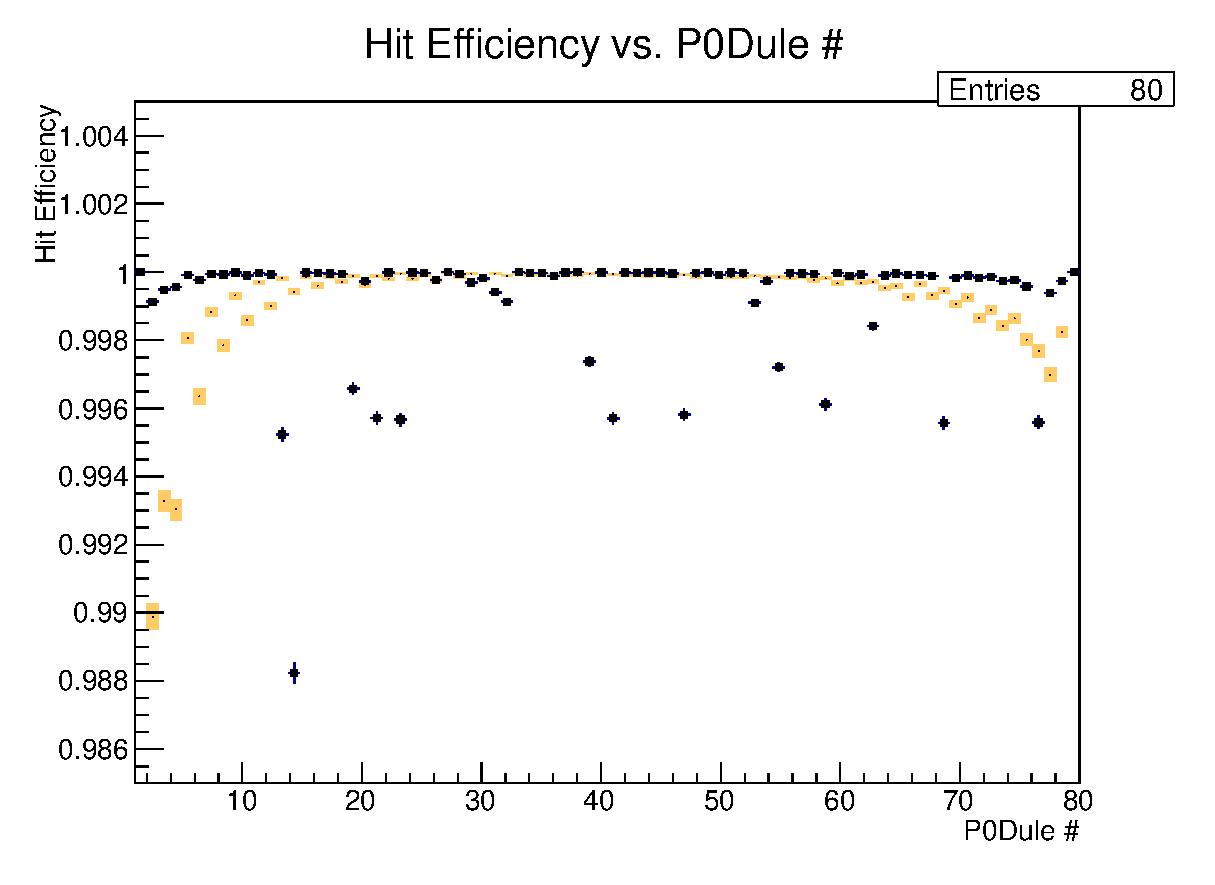
\includegraphics[width=2.5in]{Figures/Systematics/HitEfficiency/Hiteffsanda.eps}
\caption{The hit reconstruction efficiency as a function of layer number for water-in running (left) and water-out running (right). Data (black dots with error bars) and MC (orange error bars) show very high efficiencies for all layers. Layers corresponding to the water target have almost perfect efficiency. A few layers in the water target have ~0.5\% inefficiency. Note that the Y-axis is zero-suppressed.}
\label{fig:hiteffsand}
\end{figure}

\begin{table}
\centering
\begin{tabular}{lcccc}\toprule\midrule
Layer \# &  Data (Water). & MC (Water) & Data (Air) & MC (Air)  \\ \midrule
15 & 1 & 0.999894 & 0.999984 & 0.999857 \\ \midrule
65 & 0.999916 & 0.999718 & 0.99996 & 0.999587 \\ \midrule
77 & 0.999638 & 0.998028 & 0.995591 & 0.997677 \\ \midrule
78 & 0.999359 & 0.998028 & 0.999394 & 0.996979 \\ \midrule
79 & 0.999638 & 0.998416 & 0.99975 & 0.998247 \\ \midrule
%80 & 0.994044 & 0.999141  \\ \midrule
\bottomrule
\end{tabular}
\caption{Data and MC hit reconstruction efficiencies by relevant layer numbers. Errors are excluded as the efficiencies are so high. }
\label{tab:hiteff}
\end{table}


As expected, the hit reconstruction is extremely high. The few layers in Data with small ~0.5\% inefficiencies are at the single bar level, which are also expected. Any systematic arising from hit reconstruction efficiency will feed in through our matching algorithm and the Fiducial Volume cut. In the matching algorithm, we require that the \p0d track have a node in the last two p0dules, so if both p0dules somehow failed to reconstruct a node, then we would have a small inefficiency. This last two p0dules correspond to layer numbers 77-80. Also, when making the fiducial volume cut, we may misreconstruct out-of-FV tracks as in-FV due to missed nodes at the upstream end of the water target. Similarly, we may lose in-FV tracks in the downstream end of the water target. Even in the least efficient of our p0dules, failing to reconstruct two or more adjacent nodes from a track is negligible (less than 0.0025\%), so we can estimate the effect of hit reconstruction efficiency on the fiducial cut using only the likelihood of missing a single node. The upstream end of the fiducial volume corresponds to layer 15 and the downstream end corresponds to layer 65. The hit reconstruction efficiencies for layers 15, 65, and 77-80 are given in Table \ref{tab:hiteff}.

From this table, we can then extract the final systematic values due to hit reconstruction efficiency. The probability of having NO nodes in the last two layers is essentially zero and therefore not included as a systematic. The probability of having gained an out-of-FV track from the upstream end of the FV cut is given by number of muon candidate tracks originating in layer 16 multiplied by the inefficiency of layer 15. Similarly, the probability of having missed an in-FV track at the downstream end of the FV cut is given by the \# of muon candidate tracks orginating in layer 66 multiplied by the inefficiency of layer 65. The largest inefficiency is that from layer 65 in MC air running, and it is 0.04$\%$. As the change in the Data/MC ratio due to gains and losses of events from hit inefficiency cannot exceed this fraction, and is realistically smaller, we can neglect any systematic effect from hit efficiency differences between Data and MC.

\subsubsection{Neutral Back Scattering}

To be able to apply the layer efficiency study 
(Sec. \ref{sec:Systematics_HitEfficiency})
on our \p0d+TPC1 CC inclusive samples, we have preformed a similar 
layer by layer efficiency study with the CC inclusive samples. 
The efficiency study have yielded, as expected, 
very high layer efficiencies for 
both Data and MC samples.
In addition the study found that for 
a certain number of times in both beam Data and MC, 
we observe 
%large 
near the start of a track a node gaps, which is larger than 1 node.
% near the start of a track. 
We investigated these set of tracks and identified these 
gaps not to be related to layers inefficiencies. 
The investigations have found that these tracks are 
cases were an event had a
%that are not related to hit reconstruction inefficiencies. 
%Using MC, these events have been confirmed as 
neutral particle, which was back scattered from 
the interaction and converted several layers upstream 
of the true interaction vertex. 
As a result the additional hits from the converted neutral particle 
have been added to a forward going track. 
%reconstructed together with the track, 
%These additional hits have
This effect have caused the track start position to migrate  
to a an upstream location and to add layers gap in between.\\

We have further studied and looked at different properties of this topology. 
Tables \ref{tab:NodeMissFractionsWaterIn} 
and \ref{tab:NodeMissFractionsWaterOut} shows for different samples 
the fraction of tracks that have more than 1 node missed normalized 
to the number of tracks in that sample.
%Our study 
%These investigations have showed 
%have shown that 
%rates of tracks with more than 1 missing node are consistent between 
%our Data and MC samples. The 
%The fractions of tracks with more than 1 node missed 
%in Run 1 Data and MC samples are $0.90\%$ and $1.38\%$ 
%for Data and MC 
%respectively. 
For Run 1 we have found that the Data and MC fractions 
are $0.90\%$ and $1.38\%$ respectively. 
Similar behavior between Data and MC is seen at the Run 2 period 
were the fractions are $1.08\%$ and $1.40\%$ for Data and MC respectively. 
We use these fractions to find the amount in which the MC 
should be corrected, to mimic the Data, for both run periods.
The correction values we extracted are 0.13 and 0.16 events for 
Run 1 and Run 2 respectively. \\

\begin{table}[h]
\centering
\begin{tabular}{lcc}\toprule
      & &  Fraction of tracks \\
\cline{2-3}
Run 1 & Data & $1.63\%$  \\ 
      & MC & $1.90\%$  \\ 
\cline{2-3}
Run 2 & Data & $1.40\%$  \\ 
      & MC & $1.76\%$ \\ 
\cline{2-3}
Run 4 & Data & $1.39\%$  \\ 
      & MC & $1.80\%$ \\ 
\bottomrule
\end{tabular}
\caption{The fractions of tracks with more than 1 missed node 
for both Data and MC Water-in samples in the different run periods.}
\label{tab:NodeMissFractions}
\end{table}

\begin{table}[h]
\centering
\begin{tabular}{lcc}\toprule
      & &  Fraction of tracks \\
\cline{2-3}
Run 2 & Data & $1.55\%$  \\ 
      & MC & $1.83\%$  \\ 
\cline{2-3}
Run 3 & Data & $1.46\%$  \\ 
      & MC & $1.80\%$ \\ 
\cline{2-3}
Run 4 & Data & $1.65\%$  \\ 
      & MC & $1.80\%$ \\ 
\bottomrule
\end{tabular}
\caption{The fractions of tracks with more than 1 missed node 
for both Data and MC Water-out samples in the different run periods.}
\label{tab:NodeMissFractionsWaterOut}
\end{table}

\begin{figure}
\centering
\includegraphics[width=2.5in]{Figures/layerEff-5F5E-Run1-ccinc-DoMC-MissedLayerPerTracks.eps}
\includegraphics[width=2.5in]{Figures/layerEff-5F5E-Run2air-ccinc-DoMC-MissedLayerPerTracks.eps}
\includegraphics[width=2.5in]{Figures/layerEff-5F5E-Run2-ccinc-DoMC-MissedLayerPerTracks.eps}
\includegraphics[width=2.5in]{Figures/layerEff-5F5E-Run3air-ccinc-DoMC-MissedLayerPerTracks.eps}
\includegraphics[width=2.5in]{Figures/layerEff-5F5E-Run4-ccinc-DoMC-MissedLayerPerTracks.eps}
\includegraphics[width=2.5in]{Figures/layerEff-5F5E-Run4air-ccinc-DoMC-MissedLayerPerTracks.eps}
\caption{Layers distance from the first layer of missed nodes normalized 
to the number of tracks. 
The left columnb shows Water-in periods, from top to bottom 
are Run 1, Run 2 and Run 4.  
The right columb shows Water-out periods, from top to bottom 
are Run 2, Run 3 and Run 4.
In all periods 
the blue and red histograms are generated from the Data and MC samples
respectively.
}
\label{fig:MisssedNodePerTracks}
\end{figure}

Another studied aspect 
%that was studied 
was 
%the length at which the convertion occurs.
the distance of missed layers with respect to 
the first layer, the start of the track.
Fig. \ref{fig:MisssedNodePerTracks} shows the results of this study. 
%which is the frequent of a missed layer as a function of distance 
f%rom the first layer. 
The figure presents the 
missed layers distributions for both  
Data and MC samples, normalized to the number of available tracks.
One can clearly identify that the second node, 
of the tracks that had missed layers, 
% samples studied 
has the highest missed frequently. 
Another feature is the 'missed node' peak around layer 10 with 
the spread between 5 to 20 layers. 
It seem that the MC samples mimics the Data distribution 
of this feature.
Followed this spread we have calculated the number of tracks 
with missed layers, 5 to 20 layers from the start of the track 
for both run periods. 
These rates per POT are summarized 
in Tables \ref{tab:TracksWithMiss0to20perPTWaterIn} 
and \ref{tab:TracksWithMiss0to20perPTWaterOut}.
From this table one can see that the rates are similar 
between Data and MC. \\

\begin{table}[h]
\centering
\begin{tabular}{lcc}\toprule
      & &  Tracks per POT [$\times 10^{-18}$] \\
\cline{2-3}
Run 1 & Data & $6.53$  \\ 
      & MC & $7.92$ \\ 
\cline{2-3}
Run 2 & Data & $7.13$  \\ 
      & MC & $8.08$ \\ 
\cline{2-3}
Run 4 & Data & $7.52$  \\ 
      & MC & $8.12$ \\ 
\cline{2-3}
Run 1+2+4 & Data & $7.32$  \\ 
      & MC & $8.09$ \\ 
\bottomrule
\end{tabular}
\caption{The rate of tracks
with missed layers (layers 0 to 20 from counting from the start of the track)
for the Data and MC Water-in samples 
as calculated for Run 1, Run 2, Run 4 and Run 1$+$2$+$4 combined periods.
}
\label{tab:TracksWithMiss0to20perPTWaterIn}
\end{table}

\begin{table}[h]
\centering
\begin{tabular}{lcc}\toprule
      & &  Tracks per POT [$\times 10^{-18}$] \\
\cline{2-3}
Run 2 & Data & $5.38$  \\ 
      & MC & $6.34$ \\ 
\cline{2-3}
Run 3 & Data & $6.14$  \\ 
      & MC & $6.34$ \\ 
\cline{2-3}
Run 4 & Data & $5.80$  \\ 
      & MC & $6.34$ \\ 
\cline{2-3}
Run 2+3+4 & Data & $5.90$  \\ 
      & MC & $6.34$ \\ 
\bottomrule
\end{tabular}
\caption{The rate of tracks
with missed layers (layers 0 to 20 from counting from the start of the track)
for the Data and MC Water-out samples 
as calculated for Run 2, Run 3, Run 4 and Run 2$+$3$+$4 combined periods.
}
\label{tab:TracksWithMiss0to20perPTWaterOut}
\end{table}

All the above show that the skipped nodes/layers due to neutral particles 
is a small fraction of our CC inclusive sample. 
Moreover the frequencies and rates per POT of these effects 
in the MC samples look alike the Data distributions. 
These leads us to a very small systematic error contribution 
which was not included in the final summary table.

%Using beam Data and MC, we quantify both the rate of occurrence 
%of these backscattered events, as well as the characteristic length 
%at which these neutrals convert. 
%We then propagate this into an appropriate systematic 
%following the same prescription as hit reconstruction efficiency. 


\input{Sections/Systematics_FiducialMass.tex}
\subsection{Cosmics}
\label{sec:Systematics_Cosmics}

To estimate the cosmic contamination of our data samples 
we have defined the time period before the first bunch in each spill 
as a sideband sample, 
for each T2K run. \\

\begin{table}[h]
\centering
\begin{tabular}{ccccc}
%\hline
\toprule
   & & Run 1& & Run 2\\
%\hline
\cline{3-3}\cline{5-5} 
Cosmic candidate tracks& & 2 & & 0 \\
\hline 
%\cline{3-3}\cline{5-5} 
Total cosmic scanned time & & 2.429$\times 10^9$ ns & & 2.811$\times 10^9$ ns \\
\hline 
%Cosmic rate& &8.233$\cdot 10^{-10}$ track/ns& &3.557$\cdot 10^{-10}$ tracks/ns \\
%\hline 
%\cline{3-3}\cline{5-5} 
Total analysis time & & 2.159$\times 10^9$ ns & & 3.331$\times 10^9$ ns \\
\hline 
%\cline{3-3}\cline{5-5} 
Expected cosmic contamination & & 2 tracks & & 0 tracks \\
\bottomrule
\end{tabular} 
\caption{Cosmic contamination rates for the two run periods.}
\label{tab:CosmicsStudy}
\end{table}

These sideband samples were used to scan for tracks that would 
pass all of our selection cuts. 
The number of tracks found \footnote{In case no tracks were found, 
an upper limit of one track was used.} in each run is documented 
in Table \ref{tab:CosmicsStudy}. 
This number was then divided by the 'Total cosmic scanned time', 
i.e. number of spills $\times$ time period before first bunch in ns, 
to extract the rate of contaminated tracks per time unit for each run. 
To find the 'Expected cosmic contamination' number in each run, 
we multiplied the above rate by the 'Total analysis time' 
(which is the number of spills times number of bunches 
in ns). 
The results of these multiplications are rounded up 
to evaluate the number of contaminated cosmic tracks in our 
selected samples. 
Table \ref{tab:CosmicSystematics} 
summarizes all the above findings and calculations. \\

We adopt a conservative approach which assumes that when 
a contaminated track is
present in a bunch it is tagged as the muon candidate. 
We then recalculate the Data/MC ratios without these tracks and extract 
a systematic upper limit for this contamination source.

\begin{table}[h]
\centering
\begin{tabular}{ccccc}
%\hline
\toprule
   & & Run 1& & Run 2\\
\cline{3-3}\cline{5-5} 
%\cline{3-3}\cline{5-5} 
Cosmic systematics & & $-$0.00031 & & 0 \\
%\hline
\bottomrule
\end{tabular} 
\caption{Cosmic systematic values for the two run periods.}
\label{tab:CosmicSystematics}
\end{table}

We note that the study in this section has been completed with the use 
of tracks reconstructed by the Global Reconstruction package. 
The CC inclusive selection outlined in Section \ref{sec:InclusiveAnalysis} 
was performed with a Tracker to \p0d matching algorithm. 
Though these two reconstruction methods are not the exact same, 
they are very similar. In addition, from the efficiency study performed 
using cosmics (Sec. \ref{sec:CosmicsEfficiency})  
we find that the new matching algorithm maintains a high efficiency 
of reconstructing cosmics and other lengthy tracks. 
Since the overall contribution of the cosmics contamination is negligible, 
we do not expect that switching to the Tracker to \p0d matching method 
will change this systematic uncertainty. 
We adopted the conservative approach and estimate our cosmic 
systematic contribution to be $\pm0.00031$.


\subsection{Fiducial Volume}
\label{sec:Systematics_FiducialVolume}
A one-track per spill sample of beam MC has been used 
to extract the X and Y vertex resolution. 
Fig. \ref{fig:fiducialResolution} shows the X and Y coordinate resolution 
for Run 1 as determined by MC. 
The resolution is defined as the reconstructed position 
minus the true vertex position. The different X and Y resolution plots 
were fitted to a Breit-Wigner function which yielded in a FWHM 
that corresponds to a $\sigma$ of 5.7 mm and 7.2 mm respectively. \\

\begin{figure}[ht]
\centering
\includegraphics[width=2in]{Figures/P0DTrack-XResolution-Run4.eps}
\includegraphics[width=2in]{Figures/P0DTrack-YResolution-Run4.eps}
\caption{Resolution of start position of Reconstructed - MC truth. 
On the Left (Right) is the X(Y) distribution.} 
\label{fig:fiducialResolution}
\end{figure}

To extract the FV systematic values we have simultaneously varied
all of our FV boundaries 
outside and inside, 
by $\pm$10 mm (which was a conservative $\pm\sigma$) 
in both X and Y coordinates and by 
%in the case of the Z coordinate we have varied the boundaries 
$\pm 1 $ layer in the Z coordinate.
The decision to vary the Z coordinate by one readout layer 
is due to the fact that 
each \p0dule has an X layer and a Y layer, 
%, which are named 
%in the reconstruction level as X node and Y node. 
%The 
where the WT FV excludes the most upstream X layer 
and the most downstream Y layer. \\
%Therefore we have chose to vary the Z coordinate by one readout layer.\\

We recalculated our Data-to-MC ratios for the outside and inside cases 
and extracted from these the corresponding systematic values. 
Tables \ref{tab:FVSystematicsWaterIn} and \ref{tab:FVSystematicsWaterOut} 
summarizes these values for 
the combination of both Water-in and Water-out  periods respectively. 
It was found that the inside variation yielded a value of $-$0.0057 
%for both runs 
while the outside variation gave a value of $+$0.0049.
% and +0.4\% 
%for run1 and run 2 respectively.

\begin{table}[h]
\centering
\begin{tabular}{ccc}\toprule
 & & Water-in \\
%\hline
\cline{3-3}
Outside & & $+$0.00867 \\
Inside & & $-$0.00160 \\
\bottomrule
\end{tabular} 
\caption{The fiducial volume systematics for the combined 
Run 1, Run 2 and Run4 Water-in periods. 
Outside (Inside) corresponds to the case were the boundaries were 
varied outside (inside) the official ones. }
\label{tab:FVSystematicsWaterIn}
\end{table}

\begin{table}[h]
\centering
\begin{tabular}{ccc}\toprule
 & & Water-out \\
%\hline
\cline{3-3}
Outside & & $+$0.00294 \\
Inside & & $+$0.00035 \\
\bottomrule
\end{tabular} 
\caption{The fiducial volume systematics for the combined 
Run 2, Run 3 and Run4 Water-out periods. 
Outside (Inside) corresponds to the case were the boundaries were 
varied outside (inside) the official ones. }
\label{tab:FVSyatematicsWaterOut} 
\end{table}

There are a few other possible effects we must consider. One is the effect of hit reconstruction efficiency when making a FV cut. This has been shown to be negligible in Section \ref{sec:Systematics_HitEfficiency}. Another is the possibility that the vertex resolution in Data is different from that in MC. However, we note that small differences in the width of the vertex resolution will not translate to a systematic uncertainty. As long as the vertex resolution (i.e. the residual distribution) is symmetric, the number of true out-of-FV events that get `smeared' into the FV will cancel out with the number of true in-FV event that get `smeared' out of the FV. This is the case regardless of any differences between the Data and MC vertex resolution distributions. Examining the matching parameter distributions (Figures \ref{fig:eff_dR} and \ref{fig:dRetcSM}) from Sections \ref{sec:CosmicsEfficiency} and \ref{sec:SMeff}, we can draw some conclusions on the vertex resolution in data. The backwards projected Tracker track provides a best guess for where the true position of the \p0d node should be, so the $\Delta Y$ and $\Delta X$ residuals mimic the vertex resolution. We see that the Data and MC residuals have similar widths (see Table \ref{tab:FitdY} for an example) and more importantly, are symmetric. This indicates that vertex resolution has negligible effect on the Fiducial Volume systematic.



\input{Sections/Systematics_TrackTiming.tex}
\subsection{Event Pileup per Bunch}
\label{sec:Systematics_EventPileUp}
The pileup\footnote{Coincidental neutrino interactions in the same bunch.} 
event contribution in the \p0d CC inclusive samples 
should be proportional to the experimental beam power. 
From the fact that the estimated beam power used in the simulated MC 
was not the exact same as in each of the runs, we expect 
to have a different pileup effect between data and MC.
%Taken in to account the areal density of the \p0d 
%and the short time of each beam bunch, this is a small effect 
%as our study shows. 
Here we have estimated these effect difference on our 
final data to MC ratio of each run. \\

To estimate the event pileup effect we have assumed 
that there is 
an equal probability for an interaction to occur in each beam bunches. 
We can then evaluate this probability from the number of active bunches 
and the number of total bunches available for each Run both for Data and MC.
These probabilities squared are our estimations to have two 
interaction in the same bunch, i.e. the event pileup rate.
These rates were found to be very small and are summarized 
in Tables \ref{tab:PileUpEventsWaterIn} and \ref{tab:PileUpEventsWaterOut}. 
%In Run 1 extracted rates are 
%0.0000003 for Data and 0.0000005 for MC. 
%Very similar trend between a Data and MC were found in Run 2 
%i.e. 0.0000003 and 0.0000008 respectively.\\

\begin{table}[h]
\centering
\begin{tabular}{ccc}\toprule
 & & Event Pileup Fractional error \\
%\hline
\cline{3-3}
Run 1 & & $+$0.0000002 \\
Run 2 & & $+$0.000000001 \\
Run 4 & & $-$0.0000021 \\
\bottomrule
\end{tabular} 
\caption{
Event pileup fractional error on the Data/MC ratios 
as been extracted for the Water-in periods: Run 1, Run 2 and Run 4.
}
\label{tab:PileUpEventsWaterIn}
\end{table}

\begin{table}[h]
\centering
\begin{tabular}{ccc}\toprule
 & & Event Pileup Fractional error \\
%\hline
\cline{3-3}
Run 2 & & $-$0.0000008 \\
Run 3 & & $-$0.0000017 \\
Run 4 & & $-$0.0000037 \\
\bottomrule
\end{tabular} 
\caption{
Event pileup fractional error on the Data/MC ratios 
as been extracted for the Water-out periods: Run 2, Run 3 and Run 4.
}
\label{tab:PileUpEventsWaterOut}
\end{table}
 
%As in previous systematic estimations, 
%this study used Global Reconstruction as opposed to the Tracker to \p0d 
%matching algorithm used for the current CC inclusive analysis selection. 
%We do not expect coincidence rates to change appreciably from switching matching algorithms, 
%especially when the new algorithm has also demonstrated 
%to have high reconstruction efficiency. 
The systematic error on the Data to MC ratios 
for a specific run can be estimated with the use of the pileup event rates 
of both Data and MC. These were calculated for all run periods 
separately and yielded very small systematic errors 
(see Tables \ref{tab:PileUpEventsWaterIn} 
and \ref{tab:PileUpEventsWaterOut}).\\
The fact that the observed uncertainty are negligible have 
caused us not to include them in the find systematics calculation.

%estimated taking into account the spill probability factors 
%to have two interactions in two different bunches or in the same one.
%
%This, combined with the fact that the observed uncertainty is negligible, 
%allows us to quote $- 0.00005\%$, the larger of the two fractional errors 
%from Table \ref{tab:PileUpEvents}, as the event pile-up systematic.

\input{Sections/Systematics_OutofFV.tex}
\input{Sections/Systematics_TPC1tracking.tex}
\subsection{Charge Mis-ID}
\label{sec:Systematics_ChargeMisID}

We begin our study using the results of the charge mis-id study described in T2K-TN-048 v2.1 by Javier Caravaca et al. The following observations concerning our selection significantly simplify the propagation of the charge mis-ID systematic:
\begin{enumerate}
\item
The vast majority of selected muon tracks have $> 40$ nodes in the TPC constituent
\item The charge of the track is extracted only from TPC1, which makes the analysis insensitive to the global mismatching effects outlined in TN-048.
\item As the tracks have a reconstructed vertex in the \p0d, most are forward going.
\end{enumerate}

So we use Table 2 on page 8 of TN-048, which lists the charge confusion rates for TPC tracks that satisfy the requirements listed above. To propagate the charge mis-ID systematic into our analysis, we use a simple approach. We begin with samples extracted from the entire Data and Monte Carlo sets by excluding the charge cut that is the very last CC inclusive cut. So we have quality matched tracks both positive and negative that originate in the \p0d and pass through TPC1. This Data and MC sample is further classified into two mutually exclusive subsets:

\begin{enumerate}
\item Beam bunches where the highest momentum track is reconstructed as positive
\item Beam bunches where the highest momentum track is reconstructed as negative
\end{enumerate}

If a track in subset 1 had been misreconstructed as positive when in truth it was negative, then it is a candidate muon track which we missed. To correct for this, we must add the number of charge misidentified tracks in subset 1 to the total number of selected CC inlcusive events. Similarly, if a track in subset 2 had been misreconstructed as negative when in truth it was positive, then we must remove it from the number of candidate CC inclusive events. To calculate the number of tracks in each subset that were reconstructed with incorrect charge, we simply multiply by the charge mis-ID rate. So the corrected number of events after adjusting for charge mis-ID is given by:

\begin{center}
$N^{corr}(i) = N(i)+P(i)\cdot\left(N^{1}(i)-N^{2}(i)\right)$.
\end{center}

$N(i)$ is total number of events in subset 2 in a particular momentum bin $i$ and $N^{corr}(i)$ is the charge mis-ID corrected value in the same momentum bin. We chose to use subset 2 for the value of $N(i)$ as it is almost identical to the CC inclusive selection. $P(i)$ represents the probability of charge mis-ID in momentum bin $i$ extracted directly from Table 2 in TN-048 except for one small change. Negative probabilities are unphysical so we set them to 0. Any error on the probability is change to match (ex:$-0.2\pm 1$ is changed to $0 + 0.8$). Finally, $N^1$ and $N^2$ are the total number of tracks in subsets 1 and 2 respectively. Table \ref{tab:N_posneg} summarizes the number of tracks in each subset for different momentum bins in both Data and MC. Table \ref{tab:N_corr} then shows the charge mis-ID corrected number of CC inclusive events for Data and MC. 

\begin{table}
\caption{Number of Data and MC events in subset 1 and 2 for both Runs. MC values are normalized by POT, not flux-reweighted and not corrected for fiducial mass discrepancy.}
\label{tab:N_posneg}
\centering
\begin{tabular}{cccccc}\toprule
Data / MC & Mom. bin & Subset 1 & Subset 2 & Subset 1 & Subset 2\\
& Water-in & Water-in & Water-out & Water-out \\\midrule
& 0-1.3 GeV & 667 & 2463 & 1705 & 5627\\
& 1.3-2.6 GeV & 220 & 983 & 486 & 1995\\
Data & 2.6-4.0 GeV & 59 & 568 & 170 & 1290\\
& 4.0-5.3 GeV & 21 & 286 & 62 & 551\\
& 5.3+ GeV & 54 & 359 & 117 & 719 \\\midrule
& 0-1.3 GeV & 701 & 2672 & 1886 & 5959\\
& 1.3-2.6 GeV & 229 & 1025 & 547 & 2122\\
MC & 2.6-4.0 GeV & 90 & 689 & 222 & 1409\\
& 4.0-5.3 GeV & 34 & 350 & 83 & 731\\
& 5.3+ GeV & 56 & 404 & 122 & 891 \\
\bottomrule
\end{tabular}
\end{table}

\begin{table}
\caption{The charge mis-ID rate and the corrected number of CC inclusive events for Data and MC in different momentum bins for Water-in.}
\label{tab:N_corr_w}
\centering
\begin{tabular}{ccccc}\toprule
Mom. bin & Data Mis-ID Rate(\%) & MC Mis-ID Rate(\%) & $N^{corr}_{Data}$ & $N^{corr}_{MC}$ \\\midrule
0-1.3 GeV & $0+0.8$ & $0+0.1$ &2463.0 &2672.0 \\
1.3-2.6 GeV & $1.4\pm 0.7$ & $2.1\pm 0.1$  & 972.3 & 1008.5 \\
2.6-4.0 GeV & $3.3\pm 1.3$ & $4.5\pm 0.1$ & 551.2 & 661.8 \\
4.0-5.3 GeV & $6.1\pm 2.5$ & $4.5\pm 0.2$ & 269.8 & 335.9 \\
5.3+ GeV & $12\pm 3$ & $13.1\pm 0.2$  & 322.4 & 358.5 \\\midrule
Total & --  & --  & 4578.8 & 5036.7\\
\bottomrule
\end{tabular}
\end{table}

\begin{table}
\caption{The charge mis-ID rate and the corrected number of CC inclusive events for Data and MC in different momentum bins for Water-Out.}
\label{tab:N_corr_a}
\centering
\begin{tabular}{ccccc}\toprule
Mom. bin & Data Mis-ID Rate(\%) & MC Mis-ID Rate(\%) & $N^{corr}_{Data}$ & $N^{corr}_{MC}$ \\\midrule
0-1.3 GeV & $0+0.8$ & $0+0.1$ & 5627.0 & 5958.7 \\
1.3-2.6 GeV & $1.4\pm 0.7$ & $2.1\pm 0.1$  & 1973.9 & 2089.1 \\
2.6-4.0 GeV & $3.3\pm 1.3$ & $4.5\pm 0.1$ & 1253.0 & 1355.7 \\
4.0-5.3 GeV & $6.1\pm 2.5$ & $4.5\pm 0.2$ & 521.2 & 701.7 \\
5.3+ GeV & $12\pm 3$ & $13.1\pm 0.2$  & 646.8 & 791.3 \\\midrule
Total & --  & --  &10021.8 & 10896.6\\
\bottomrule
\end{tabular}
\end{table}

To extract systematics from Tables \ref{tab:N_corr_w} and \ref{tab:N_corr_a}, we recalculate the Data/MC ratio with the corrected values and take the difference from the nominal ratio. The nominal ratio is defined as the Data/MC ratio from the total number of events in subset 2. %The nominal ratio is 98.23\% and the corrected ratio is 98.56\%, which yields a systematic difference of 0.33\%.
The errors on the charge mis-ID values are on the order of the misidentification rate itself, so we cannot ignore them. To be conservative, we linearly added and subtracted the mis-ID rate with the error in each bin. Any negative probabilities were set to 0. The change in Data/MC ratio was calculated for both the cases where all the mis-ID rates had gone up by 1 $\sigma$ and gone down by 1 $\sigma$. The larger change is assigned as a symmetric systematic error. We find a systematic of $\pm 0.75\% $ and $\pm 0.72\%$ from the charge mis-ID rate for water-in and water-out running respectively.

\clearpage
\input{Sections/Systematics_Summary_2.tex}
\section{Results and Discussion}
\label{sec:results}

In this thesis we have presented a measurement of the $\nu_\mu$ induced flux-averaged, charged current inclusive, absolute cross section on water. We use data from all four beam run periods with an accumulated exposure of 5.636$\times 10^{20}$ protons on target. Charged current inclusive events are selected in the water target volume of the P0D by requiring the produced muon to pass through the Tracker that is directly downstream. Data is collected from the P0D while it is both filled with water and drained of water. The background contamination and the signal efficiency are both estimated using NEUT MC. After background subtracting and efficiency correcting the water-in and water-out CC inclusive event rates, we perform a statistical subtraction to extract the absolute water cross section.

There are several detector level corrections that are made. Specifically, the MC estimations for background and signal efficiency are corrected for small differences between data and MC in the P0D fiducial mass, the track matching efficiency, and the sand muon interference rate. These corrections shift the central value of the absolute water cross section by a small amount. Many sources of systematic uncertainty have also been evaluated. These include the flux systematic uncertainty, the standard interaction cross section model uncertainty, the final state interaction cross section model uncertainty and a host of detector level systematic uncertainties. Fractionally, the flux, physics model and detector systematic uncertainties are $^{-9.62\%}_{+11.09\%}$, $^{-13.43\%}_{+8.79\%}$ and $\pm 2.02\%$ respectively. This yields a total systematic uncertainty of $-16.64\%$ and $+14.29\%$ fractionally.

As our analysis studies charged current interactions and we do not distinguish interactions on protons and neutrons, our result is a cross section measurement per nucleon. However, water is not an iso-scalar target, so the result is given per H$_2$O nucleon. We also include a result per water molecule. The final, $\nu_\mu$ induced, flux-averaged CC inclusive absolute water cross section is:

\begin{equation}
\left<\sigma\right>_\Phi = (6.37 \pm 0.157 (stat.) ^{-1.060}_{+.910} (sys.))\times 10^{-39} \frac{\text{cm}^2}{H_2O\:\text{nucleon}}
\end{equation}

\begin{equation}
\left<\sigma\right>_\Phi = (11.5 \pm 0.284 (stat.) ^{-1.91}_{+1.64} (sys.))\times 10^{-38} \frac{\text{cm}^2}{H_2O\:\text{molecule}}
\end{equation}

To compare to other results from different neutrino experiments, it is useful to convert our cross section measurement to that on an iso-scalar target such as carbon. The inclusive charged current cross section of a neutrino with a neutron has been observed to be higher than that of a neutrino with a proton. An iso-scalar target has the same number of neutrons and protons, so to compare to such a target, we must average out the structure of our own nucleus. In water, there are 10 protons and 8 neutrons, so we use the following correction formula:

\begin{equation}
\left<\sigma\right>_\Phi^{iso} = \left<\sigma\right>_\Phi^{H_2O}*\frac{(10\sigma(\nu p)+8\sigma(\nu n))/18}{(\sigma(\nu p)+\sigma(\nu n))/2}
\end{equation}
where $\sigma(\nu p)$ and $\sigma(\nu n)$ are the CC inclusive cross sections on protons and neutrons individually. We use a  $\sigma(\nu n)/\sigma(\nu p)$ ratio of 3.3 to calculate the corrected cross section per iso-scalar nucleon for comparison. The value of 3.3 was extracted from a digitized plot of the BNL-7ft experiment results that measure the relative neutron and proton cross sections. Note that as we expect some coherent neutrino interactions, this iso-scalar conversion does not account for nuclear effects.

The $\nu_\mu$ induced, flux-averaged CC inclusive absolute water cross section per iso-scalar nucleon is:

\begin{equation}
\left<\sigma\right>_\Phi^{iso} = (6.77 \pm 0.167 (stat.) ^{-1.127}_{+.968} (sys.))\times 10^{-39} \frac{\text{cm}^2}{\text{iso. nucleon}}.
\end{equation}
This result can be compared to the result from Ref\cite{ccinc} that used the Tracker for a similar CC inclusive selection on primarily carbon which is an iso-sclar target. The analysis in Ref\cite{ccinc} has a higher efficiency of high-angle and low momentum muon tracks. They find a flux averaged CC inclusive cross section of $(6.93 \pm 0.13 (stat.) \pm 0.85(sys.)) \times 10^{-39} \frac{cm^2}{nucleons}$. These results are quite compatible as we would expect. Note that the flux and model systematics are very highy correlated between these two measurements. We can also compare our iso-scalar result with the NEUT and GENIE predictions in Ref\cite{ccinc}. They predict that the cross sections are:

\begin{equation}
\left<\sigma\right>_\Phi^{NEUT} = 7.26 \times 10^{-39} \frac{cm^2}{nucleon}
\end{equation}

\begin{equation}
\left<\sigma\right>_\Phi^{GENIE} = 6.68 \times 10^{-39} \frac{cm^2}{nucleon}
\end{equation}

For comparison with other data, we present our result and the NEUT/GENIE predictions as a cross section per GeV. The P0D T2K result is shown in figure \ref{fig:xsdata} overlaid on results from several other experiments. The colored lines show the NEUT and GENIE predictions for T2K as extracted from Ref \cite{ccinc}. Some of the data were digitized directly from the relevant publications and others were taken from tables or data releases. We have marked the data sets that were collected through digitization in the figure. Furthermore, many results were quoted as an absolute cross section instead of cross section divided by neutrino energy. We took a direct division of the cross section and the mean neutrino energy without adding any neutrino energy shape errors to the systematic envelope of the divided result. The neutrino energy shape errors should be accounted for in the horizontal error bars. Finally, for a few data points, we do not show a horizontal error bar. This is either a result of no horizontal errors being provided or no meaningful digitization of horizontal error bars being available in the publications. In our case, it is a nontrivial matter to calculate an error envelope on the neutrino flux. We do not provide one in this plot. For the mean neutrino energy of T2K, we use the value of 0.85~GeV \cite{ccinc}.

We find that our error bars are comparable to the most precise measurements of neutrino cross section at such low energies. We are also consistent with global data and the GENIE cross section prediction. We are also the very first inclusive charged current cross section result on the non-isoscalar target of water, a common target in many neutrino detectors. In the future, we can hope to extract the ratios of exclusive neutrino interactions and to compare nuclear effects on a water molecule. We can also, with better reconstruction techniques, achieve higher efficiencies at steeper muon angles and lower neutrino energies. Finally, with the proper treatment of migration errors, it is also possible to extend this result into multiple bins of muon kinematic observables to extract a single or double differential cross section on water.
\afterpage{
\begin{landscape}
\begin{figure}[h]
\centering
$\vcenter{\hbox{\includegraphics[height=5.5in]{Figures/XSec.png}}}$
\caption{Absolute neutrino cross sections divided by mean neutrino energy for various experiments. The result from this analysis is shown in blue with total vertical error bars. No error on the mean neutrino energy is shown. Experiment names marked with (*) have data extracted from plots by digitization. The MC predictions are taken directly from digitizing the NEUT/GENIE figure from Ref\cite{ccinc}.}
\label{fig:xsdata}
\end{figure}
\end{landscape}
}

\begin{thebibliography}{99}

\bibitem{p0dNIM}
 S.~Assylbekov, G.~Barr, B.~E.~Berger{\it et al.},
{\it``The T2K ND280 Off-Axis Pi-Zero Detector''},
  Nucl.\ Instrum.\ Meth.\ A {\bf 686}, 48 (2012); 
  [arXiv:1111.5030 [physics.ins-det]].
\bibitem{tn73}
K. Gilije, {\it Fiducial Mass Calculation}, T2K-TN-073.
\bibitem{tn72}
A. Hillairet, {\it et al.}, {\it ND280 Reconstruction}, T2K-TN-072.
\bibitem{bayes}
M. Paterno, {\it Calculating Efficiencies and Their Uncertainties}, http://home.fnal.gov/~paterno/images/effic.pdf
\bibitem{tn48}
J. Caravaca, {\it Charge Misidentification in local and global reconstruction}, T2K-TN-048
\bibitem{tn43}
A. Hillairet, {\it Track-finding inefficiency in the TPC reconstruction}, T2K-TN-043
\bibitem{bayes}
M. Paterno, {\it Calculating Efficiencies and Their Uncertainties}, http://home.fnal.gov/~paterno/images/effic.pdf
\bibitem{tn88}
O. Perevozchikov, {\it Magnet Induced background for neutrino interactions 
and C analysis in SMRD}, T2K-TN-088.
\bibitem{neut}
Y. Hayato, {\it A Neutrino Interaction Simulation Program Library NEUT}, Acta Phys. Pol. B40, 2477 (2009).


\end{thebibliography}

\renewcommand{\thesubsection}{\Alph{subsection}}
\section{Appendix}
\label{sec:appendix}


\begin{figure}[H]
\centering
\includegraphics[width=5in]{Figures/TN100Plots/c_7_0.png}
\caption{The fractional change in water-in signal efficiency (predicted from MC) as a function of Muon Momentum for a +1$\sigma$ (blue) and -1$\sigma$ (red) variation of cross section parameter. From left to right, top to bottom, the cross section parameters varied are: MAQE, MARES, DIS Multi-Pi Shape, Spectral Function, Fermi Momentum, Pion-less Delta Decay, CCQE Norm. ($E_\nu < 1.5$GeV), CCQE Norm. ( 3.5~GeV$E_\nu>1.5$GeV), CCQE Norm ($E_\nu > 3.5$GeV), CC 1Pi Norm. ($E_\nu < 2.5$GeV), CC 1Pi Norm. ($E_\nu > 2.5$GeV), CC Coh Norm., NC Coh Norm., NC 1Pi Norm., NC Other Norm., MiniBoone CC 1Pi $E_\nu$ Shape.}
\label{fig:xsvarPwE}
\end{figure}

\begin{figure}[H]
\centering
\includegraphics[width=5in]{Figures/TN100Plots/c_13_0.png}
\caption{The fractional change in the water-in background (predicted from MC) as a function of Muon Momentum for a +1$\sigma$ (blue) and -1$\sigma$ (red) variation of cross section parameter. From left to right, top to bottom, the cross section parameters varied are: MAQE, MARES, DIS Multi-Pi Shape, Spectral Function, Fermi Momentum, Pion-less Delta Decay, CCQE Norm. ($E_\nu < 1.5$GeV), CCQE Norm. ( 3.5~GeV$E_\nu>1.5$GeV), CCQE Norm ($E_\nu > 3.5$GeV), CC 1Pi Norm. ($E_\nu < 2.5$GeV), CC 1Pi Norm. ($E_\nu > 2.5$GeV), CC Coh Norm., NC Coh Norm., NC 1Pi Norm., NC Other Norm., MiniBoone CC 1Pi $E_\nu$ Shape.}
\label{fig:xsvarPwB}
\end{figure}

\begin{figure}[H]
\centering
\includegraphics[width=5in]{Figures/TN100Plots/c_8_0.png}
\caption{The fractional change in the water-in signal efficiency (predicted from MC) as a function of Muon Track Theta for a +1$\sigma$ (blue) and -1$\sigma$ (red) variation of cross section parameter. From left to right, top to bottom, the cross section parameters varied are: MAQE, MARES, DIS Multi-Pi Shape, Spectral Function, Fermi Momentum, Pion-less Delta Decay, CCQE Norm. ($E_\nu < 1.5$GeV), CCQE Norm. ( 3.5~GeV$E_\nu>1.5$GeV), CCQE Norm ($E_\nu > 3.5$GeV), CC 1Pi Norm. ($E_\nu < 2.5$GeV), CC 1Pi Norm. ($E_\nu > 2.5$GeV), CC Coh Norm., NC Coh Norm., NC 1Pi Norm., NC Other Norm., MiniBoone CC 1Pi $E_\nu$ Shape.}
\label{fig:xsvarTwE}
\end{figure}

\begin{figure}[H]
\centering
\includegraphics[width=5in]{Figures/TN100Plots/c_14_0.png}
\caption{The fractional change in the water-in background (predicted from MC) as a function of Muon Track Theta for a +1$\sigma$ (blue) and -1$\sigma$ (red) variation of cross section parameter. From left to right, top to bottom, the cross section parameters varied are: MAQE, MARES, DIS Multi-Pi Shape, Spectral Function, Fermi Momentum, Pion-less Delta Decay, CCQE Norm. ($E_\nu < 1.5$GeV), CCQE Norm. ( 3.5~GeV$E_\nu>1.5$GeV), CCQE Norm ($E_\nu > 3.5$GeV), CC 1Pi Norm. ($E_\nu < 2.5$GeV), CC 1Pi Norm. ($E_\nu > 2.5$GeV), CC Coh Norm., NC Coh Norm., NC 1Pi Norm., NC Other Norm., MiniBoone CC 1Pi $E_\nu$ Shape.}
\label{fig:xsvarTwB}
\end{figure}

\begin{figure}[H]
\centering
\includegraphics[width=5in]{Figures/TN100Plots/c_9_0.png}
\caption{The fractional change in the water-in signal efficiency (predicted from MC) as a function of X position of the vertex for a +1$\sigma$ (blue) and -1$\sigma$ (red) variation of cross section parameter. From left to right, top to bottom, the cross section parameters varied are: MAQE, MARES, DIS Multi-Pi Shape, Spectral Function, Fermi Momentum, Pion-less Delta Decay, CCQE Norm. ($E_\nu < 1.5$GeV), CCQE Norm. ( 3.5~GeV$E_\nu>1.5$GeV), CCQE Norm ($E_\nu > 3.5$GeV), CC 1Pi Norm. ($E_\nu < 2.5$GeV), CC 1Pi Norm. ($E_\nu > 2.5$GeV), CC Coh Norm., NC Coh Norm., NC 1Pi Norm., NC Other Norm., MiniBoone CC 1Pi $E_\nu$ Shape.}
\label{fig:xsvarXwE}
\end{figure}

\begin{figure}[H]
\centering
\includegraphics[width=5in]{Figures/TN100Plots/c_15_0.png}
\caption{The fractional change in the water-in background (predicted from MC) as a function of X position of the vertex for a +1$\sigma$ (blue) and -1$\sigma$ (red) variation of cross section parameter. From left to right, top to bottom, the cross section parameters varied are: MAQE, MARES, DIS Multi-Pi Shape, Spectral Function, Fermi Momentum, Pion-less Delta Decay, CCQE Norm. ($E_\nu < 1.5$GeV), CCQE Norm. ( 3.5~GeV$E_\nu>1.5$GeV), CCQE Norm ($E_\nu > 3.5$GeV), CC 1Pi Norm. ($E_\nu < 2.5$GeV), CC 1Pi Norm. ($E_\nu > 2.5$GeV), CC Coh Norm., NC Coh Norm., NC 1Pi Norm., NC Other Norm., MiniBoone CC 1Pi $E_\nu$ Shape.}
\label{fig:xsvarXwB}
\end{figure}

\begin{figure}[H]
\centering
\includegraphics[width=5in]{Figures/TN100Plots/c_10_0.png}
\caption{The fractional change in the water-in signal efficiency (predicted from MC) as a function of Y position of the vertex for a +1$\sigma$ (blue) and -1$\sigma$ (red) variation of cross section parameter. From left to right, top to bottom, the cross section parameters varied are: MAQE, MARES, DIS Multi-Pi Shape, Spectral Function, Fermi Momentum, Pion-less Delta Decay, CCQE Norm. ($E_\nu < 1.5$GeV), CCQE Norm. ( 3.5~GeV$E_\nu>1.5$GeV), CCQE Norm ($E_\nu > 3.5$GeV), CC 1Pi Norm. ($E_\nu < 2.5$GeV), CC 1Pi Norm. ($E_\nu > 2.5$GeV), CC Coh Norm., NC Coh Norm., NC 1Pi Norm., NC Other Norm., MiniBoone CC 1Pi $E_\nu$ Shape.}
\label{fig:xsvarYwE}
\end{figure}

\begin{figure}[H]
\centering
\includegraphics[width=5in]{Figures/TN100Plots/c_16_0.png}
\caption{The fractional change in the water-in background (predicted from MC) as a function of Y position of the vertex for a +1$\sigma$ (blue) and -1$\sigma$ (red) variation of cross section parameter. From left to right, top to bottom, the cross section parameters varied are: MAQE, MARES, DIS Multi-Pi Shape, Spectral Function, Fermi Momentum, Pion-less Delta Decay, CCQE Norm. ($E_\nu < 1.5$GeV), CCQE Norm. ( 3.5~GeV$E_\nu>1.5$GeV), CCQE Norm ($E_\nu > 3.5$GeV), CC 1Pi Norm. ($E_\nu < 2.5$GeV), CC 1Pi Norm. ($E_\nu > 2.5$GeV), CC Coh Norm., NC Coh Norm., NC 1Pi Norm., NC Other Norm., MiniBoone CC 1Pi $E_\nu$ Shape.}
\label{fig:xsvarYwB}
\end{figure}

\end{document}
